%%%%%%%%%%%%%%%%%%%%%%% file template.tex %%%%%%%%%%%%%%%%%%%%%%%%%
%
% This is a general template file for the LaTeX package SVJour3
% for Springer journals.          Springer Heidelberg 2010/09/16
%
% Copy it to a new file with a new name and use it as the basis
% for your article. Delete % signs as needed.
%
% This template includes a few options for different layouts and
% content for various journals. Please consult a previous issue of
% your journal as needed.
%
%%%%%%%%%%%%%%%%%%%%%%%%%%%%%%%%%%%%%%%%%%%%%%%%%%%%%%%%%%%%%%%%%%%
%
% First comes an example EPS file -- just ignore it and
% proceed on the \documentclass line
% your LaTeX will extract the file if required
\begin{filecontents*}{example.eps}
%!PS-Adobe-3.0 EPSF-3.0
%%BoundingBox: 19 19 221 221
%%CreationDate: Mon Sep 29 1997
%%Creator: programmed by hand (JK)
%%EndComments
gsave
newpath
  20 20 moveto
  20 220 lineto
  220 220 lineto
  220 20 lineto
closepath
2 setlinewidth
gsave
  .4 setgray fill
grestore
stroke
grestore
\end{filecontents*}
%
\RequirePackage{fix-cm}
%
%\documentclass{svjour3}                     % onecolumn (standard format)
%\documentclass[smallcondensed]{svjour3}     % onecolumn (ditto)
%\documentclass[smallextended]{svjour3}       % onecolumn (second format)
\documentclass[twocolumn]{svjour3}          % twocolumn
%
\smartqed  % flush right qed marks, e.g. at end of proof
%
\usepackage{graphicx}
\usepackage{times}
\usepackage{epsfig}
\usepackage{epstopdf}
\usepackage{amsmath}
\usepackage{amssymb}
\usepackage{subfigure}
\usepackage{caption}
\usepackage{tabularx}
\usepackage[table]{xcolor}
%
% \usepackage{mathptmx}      % use Times fonts if available on your TeX system
%
% insert here the call for the packages your document requires
%\usepackage{latexsym}
% etc.
%
% COLORS
\definecolor{myGreen}{HTML}{33FF00}
\definecolor{myRed}{HTML}{FF3030}
% please place your own definitions here and don't use \def but
% \newcommand{}{}
\newcommand{\PP}{\mathbb{P}}
\newcommand{\Ncal}{N_{\text{c}}}
\newcommand{\subw}{0.20\linewidth}
\newcommand{\wii}{0.323\linewidth}
\newcommand{\myCap}
{
   {\bf  A visualization of learnt feature wights for two database images. In each panel:} 
   \emph{first~row:} (Right) Target database image $j$. (Left) Cumulative density function (or calibrated score) learnt for the SVM scores of the corresponding classifier $f_j$;  three query images displayed on the \emph{second row} are represented by their SVM scores and cdf values $F_0(s)$, denoted (a)-(c) on the graph. \emph{Third~row:} A visualization of the contribution of each feature to the SVM score for the corresponding query image. Red circles represent features with negative weights while green circles correspond to features with positive weights. The area of each circle is proportional to the contribution of the corresponding feature to the SVM score.

   Notice that the correctly localized queries (c) contain more green colored features than queries from other places (b) and (a).
   {\it Left panel:}
   Query (b) gets a high score because the building has orange and white stripes similar to the the sun-blinds of the bakery, which are features that also have large positive weights in the query image (c) of the correct place.
   {\it Right panel:}
   Query (b) is in fact also an image of the same location with a portion of the left skyscraper in the target image detected in the upper left corner and the side of the rightmost building in the target image detected in the top right corner. Both are clearly detected by the method as indicated by a large quantity of green circles in the corresponding regions.
}
%
% Insert the name of "your journal" with
\journalname{IJCV}
%
\begin{document}

\title{Learning and calibrating per-location classifiers for visual place recognition\thanks{Grants or other notes
about the article that should go on the front page should be
placed here. General acknowledgments should be placed at the end of the article.}
}
\subtitle{...and embedding compact descriptors}

%\titlerunning{Short form of title}        % if too long for running head

\author{Petr Gron{\'a}t         \and
        Josef {S}ivic          \and
        Tom{\'a}{\v s} Pajdla%etc.
}

%\authorrunning{Short form of author list} % if too long for running head

\institute{F. Author \at
              first address \\
              Tel.: +123-45-678910\\
              Fax: +123-45-678910\\
              \email{fauthor@example.com}           %  \\
%             \emph{Present address:} of F. Author  %  if needed
           \and
           S. Author \at
              second address
}

\date{Received: date / Accepted: date}
% The correct dates will be entered by the editor
%\maketitle
%***********************************************************
% *** THIS puts a figure between title and abstract ***
\twocolumn
[{%
    \renewcommand\twocolumn[1][]{#1}%
    \maketitle
    \begin{center}
        \centering
        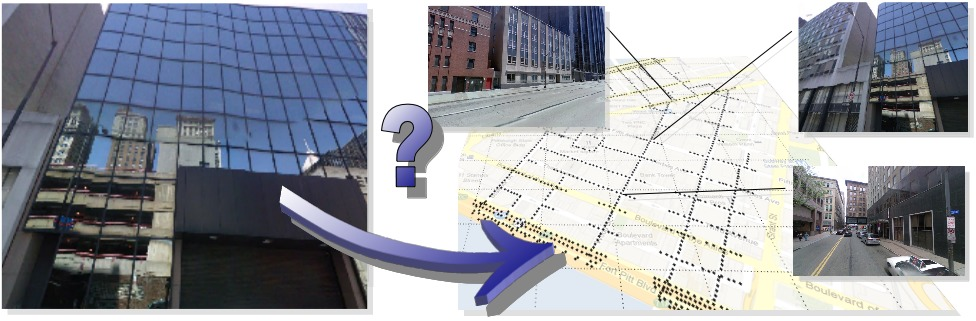
\includegraphics[width=.85\textwidth]{imgs/titleTeX.png}
        \vspace*{-3mm}
        \captionof{figure}
        {
          The goal of this work is to localize a query photograph (left) by finding other images of the same place in a large geotagged image database (right). 
          We cast the problem as a classification task and learn a classifier for each location in the database. We develop a non-parametric procedure to calibrate the outputs of the large number of per-location classifiers without the need for additional positive training data.  
        }
    \end{center}%
}]
% ******************************************************

%\maketitle

\begin{abstract}
The aim of this work is to localize a query photograph by finding other images depicting the same place in a large geotagged image database. 
This is a challenging task due to changes in viewpoint, imaging conditions and the large size of the image database. The contribution of this work is two-fold. First, we cast the place recognition problem as a classification task and use the available geotags to train a classifier for each location in the database in a similar manner to per-exemplar SVMs in object recognition. Second, as only few positive training examples are available for each location, we propose a new approach to calibrate all the per-location SVM classifiers using \emph{only} the negative examples. The calibration we propose relies on a significance measure essentially equivalent to the p-values classically used in statistical hypothesis testing. Experiments are performed on a database of 25,000 geotagged street view images of Pittsburgh and demonstrate improved place recognition accuracy of the proposed approach over the previous work.
\keywords{Place recognition \and SVM calibration \and Geo-location}
% \PACS{PACS code1 \and PACS code2 \and more}
% \subclass{MSC code1 \and MSC code2 \and more}
\end{abstract}
%%%%%%%%%%%%%%%%%%%%%%%%
\section{Introduction}
%%%%%%%%%%%%%%%%%%%%%%%%
   \label{intro}
   Visual place recognition~\cite{Cummins09,Knopp2010,Schindler07} is a challenging task as the query and database images may depict the same 3D structure (e.g.\ a building) from a different camera viewpoint, under different illumination, or the building can be partially occluded. 
   In addition, the geotagged database may be very large. For example, we estimate that Google street-view of France alone contains more than 60 million panoramic images.

   Similar to other work in large scale place recognition~\cite{Cummins09,Knopp2010,Schindler07} and image retrieval~\cite{Nister06,Philbin07,Sivic2003}, we build on the bag-of-visual-words representation~\cite{Csurka04,Sivic2003} and describe each image by a set of quantized local invariant features, such as SURF~\cite{Bay06} or SIFT~\cite{Lowe04}.  Each image is then represented by a weighted histogram of visual words, called the ``tf-idf vector'' due to the commonly used tf-idf weighting scheme~\cite{Sivic2003}. The vectors are usually normalized to have unit $L_2$ norm and the similarity between the query and a database vector is then measured by their dot product. This representation has some desirable properties such as robustness to background clutter and partial occlusion. Efficient retrieval is then achieved using inverted file indexing. 

   Recent work has looked at different ways to improve the retrieval accuracy and speed of the bag-of-visual-words model for image and object retrieval. Examples include: 
   (i) learning better visual vocabularies from training examples with matched/non-matched descriptors~\cite{Mikulik2010,Philbin10b}; 
   (ii)  developing quantization methods less prone to quantization errors~\cite{Jegou2011,Philbin08} or 
   (iii) combining results from multiple query images depicting the same scene~\cite{Chum11,Chum07b}.

   While in image retrieval  databases are typically unstructured collections of images, place recognition databases are usually structured: images have geotags, are localized on a map and depict a consistent 3D world. %~\cite{Gronat2011}. 
   Knowing the structure of the database can lead to significant improvements in both speed and accuracy of place recognition. 
   Examples include: (i) building an explicit 3D reconstruction of the scene~\cite{Irschara2009,Li10,Li12}; (ii) constructing an image graph~\cite{Philbin10c,Turcot09}, where images are nodes and edges connect close-by images on the map~\cite{Torii11}, or (iii) using the geotagged data as a form of supervision to select local features that characterize a certain location~\cite{Knopp2010,Schindler07} or re-rank retrieved images~\cite{Zamir10}.

   In this work, we also take advantage of geotags as an available form of supervision and investigate whether the place recognition problem can be cast as a classification task.
   While visual classifiers were investigated for landmark recognition~\cite{Li09}, where many photographs are available for each of the landmarks, in this work we wish to train a classifier {\em for each location on the map} in a similar manner to per-exemplar classification in object recognition~\cite{Malisiewicz11}. This is beneficial as  each classifier can learn which features are discriminative for a particular place. % and down-weight features occurring at other places.
   The classifiers are learnt offline. At query time, the query photograph is localized by transferring the GPS tag of the best scoring location classifier.

   While learning classifiers for each place may be appealing, calibrating outputs of the individual classifiers is a critical issue. In object recognition~\cite{Malisiewicz11}, it is addressed in a separate calibration stage on a held-out set of training data.
   This is not possible in the place recognition set-up as only a small number, typically one to five, of positive training images are available for each location (e.g. street-view images viewing the same building facade). To address this issue, we propose a calibration procedure inspired by the use of p-values in statistics and based on ranking the score of a query image amongst scores of other images in the database.

   The rest of the paper is organized as follows: Section~\ref{sec:classifiers} describes how per-location classifiers are learnt. Section~\ref{sec:calibration} details the classifier calibration procedure.   Implementation details and experimental results are given in Section~\ref{sec:experiments}.

%%%%%%%%%%%%%%%%%%%%%%%%
\section{Per-location classifiers for place recognition}
\label{sec:classifiers}
%%%%%%%%%%%%%%%%%%%%%%%%
   We are given tf-idf vectors $d_j$, one for each database image $j$. The goal is to learn a score $f_j$ for each database image $j$, so that, at test time, given the descriptor $q$ of the query image, we can either retrieve the correct target image as the image $j^*$ with the highest score 
   \begin{equation}
   \label{eq:class}
    j^*=\operatorname*{arg\;max}_{j} f_j(q) 
   \end{equation}

   \noindent
   or use these scores to rank candidate images and use geometric verification to try and identify the correct location in an $n$-best list.
   Instead of approaching the problem directly as a large multiclass classification problem, we tackle the problem by learning a per-exemplar linear SVM classifier~\cite{Malisiewicz11}  for each database image $j$.
   Similar to~\cite{Knopp2010}, we use the available geotags to construct the negative set $\mathcal N_j$ for each image $j$. The negative set is constructed so as to concentrate difficult negative examples, i.e.\ from images that are far away from the location of image $j$ and at the same time similar to the target image as measured by the dot product between their feature vectors. The details of the construction procedure will be given in section~\ref{sec:experiments}.  The positive set $\mathcal P_j$ is represented by the only positive example, which is $d_j$ itself. 

   Each SVM classifier produces a score $s_j$ which is a priori not comparable with the score of the other classifiers. A calibration of these scores will therefore be key to convert them to comparable scores $f_j$. This calibration problem is more difficult than usual given that we only have a single positive example and will be addressed in section~\ref{sec:calibration}.
   %%%%%%%%%%%%%%%%%%%%%%%%%%%%%%%%%%%%%%%%%%%%%%%%%%%
   \paragraph{Learning per-location SVM classifiers. }
   %%%%%%%%%%%%%%%%%%%%%%%%%%%%%%%%%%%%%%%%%%%%%%%%%%%
      Each linear SVM classifier learns a score $s_j$ of the form 

      \begin{equation}
       \label{eq:linear}
        s_j(q)=w_j^T q+b_j
      \end{equation}

      \noindent
      where $w_j$ is a weight vector re-weighting contributions of individual visual words and $b_j$ is the bias specific for image $j$. Given the training sets $\mathcal P_j$ and $\mathcal N_j$, the aim is to find a vector $w_j$ and bias $b_j$ such that the score difference between $d_j$ and the closest neighbor from its negative set $\mathcal N_j$ is {\em maximized}. Learning the weight vector $w_j$ and bias $b_j$ is formulated as a minimization of the convex objective 

      \begin{align}
        \nonumber
        \Omega(w_j,b_j)=||w_j||^{2}& +C_1\sum_{x\in \mathcal P_j}h(w_j^Tx+b_j)   \\
        \label{eq:obj}
                           & +C_2\sum_{x\in \mathcal N_j}h(-w_j^Tx-b_j), 
      \end{align}

      \noindent
      where the first term is the regularizer, the second term is the loss on the positive training data weighted by scalar parameter $C_1$, and the third term is the loss on the negative training data weighted by scalar parameter $C_2$.   
      This is a standard SVM formulation \eqref{eq:obj}, also used in exemplar-SVM~\cite{Malisiewicz11}.
      In our case $h$ is the squared hinge loss, which we found to work better in our setting than the standard hinge-loss. $w_j$ and $b_j$ are learned separately for each database image $j$ in turn. 
      In our case (details in section~\ref{sec:experiments}), we use about 1-5 positive examples, and 200 negative examples. As the dimensionality of $w$ is $100,000$ all training data points are typically support vectors. 
   %%%%%%%%%%%%%%%%%%%%%%%%%%%%%%%%%%%%%%%
   \paragraph{Expanding the positive set.}
   %%%%%%%%%%%%%%%%%%%%%%%%%%%%%%%%%%%%%%%
      A typical geotagged database may contain several images depicting a particular location. For example, neighboring street-view panoramas depict the same store front from different viewpoints. However, a specific place is often imaged only in a small number (2-5) of neighboring panoramas. 
      If such images are identified, they may provide a few additional positive examples for the particular place and improve the quality of that per-location classifier. Moreover, treating them erroneously as negatives is likely to bias the learnt classifier.
      We automatically identify such images as geo-graphically close-by images to the location $j$.
      These images can be further verified using geometric verification~\cite{Philbin07} and included in the positive training data for location $j$. Details are given in section~\ref{sec:experiments}.
  %%%%%%%%%%%%%%%%%%%%%%%%%%%%%%%%%%%%%%%
  \paragraph{Dual representation.}
  %%%%%%%%%%%%%%%%%%%%%%%%%%%%%%%%%%%%%%% 
      For each image $j$ in the database the linear SVM \ref{eq:linear} is learned. The image is then represented by corresponding weight $w_j$ and bias $b_j$. The main drawback is that while the original high dimensional tf-idf vector $d_j$ was sparse the learned weight vector $w_j$ is dense. Hence a memory requirement for storage of the new representation is enormous.

      Since the number of training data $k$ is significantly lower then the dimensionality $d$ of the vector $w$ one can benefit from the dual representation. As $d>>k$ all the training data are typically support vectors and each vector $w$ can be expressed in dual form as

      \begin{equation}
        w=\sum_{i\in \mathcal{P},\mathcal{N}} \alpha_i d_i = D \cdot \vec{\alpha}
      \end{equation}

      \noindent
      where $\alpha_i$ are coefficients of linear combination of training data $d_i$. A column wise matrix $W$ that contains all learned weights can be then expressed in matrix form as follows

      \begin{equation}
        W=D*A  
      \end{equation}


%%%%%%%%%%%%%%%%%%%%%%%%%%  
\section{Non-parametric calibration of the  SVM-scores from negative examples only}
\label{sec:calibration}
%%%%%%%%%%%%%%%%%%%%%%%%%%  
   Since the classification scores $s_j$ are learned independently for each location $j$, they cannot be directly used as the scores $f_j$ from eq.~\eqref{eq:class}. As illustrated in figure~\ref{fig:calib}, for a given query $q$, a classifier from an incorrect location (b) can have a higher score~\eqref{eq:linear} than the classifier from the target location (a). Indeed, the SVM score is a signed distance from the discriminating hyperplane and is a priori not comparable between different classifiers. This issue is addressed by calibrating scores of the learnt classifiers. The goal of the calibration is to convert the output of each classifier into a probability (or in general a ``universal" score), which can be meaningfully compared across classifiers. 

   Several calibration approaches have been proposed in the literature (see~\cite{gebel2007calibrating} and references therein for a review). The most known consists of fitting a logistic regression to the output of the SVM~\cite{Platt99}.  This approach, however, has a major drawback as it imposes a parametric form (the logistic a.k.a.\ sigmoid function) of the likelihood ratio of the two classes, which typically leads to biased estimates of the calibrated scores. Another important calibration method is the isotonic regression~\cite{zadrozny2002transforming}, which allows for a non-parametric estimate of the output probability.
   Unfortunately, the fact that we have only a single positive example (or only very few of them, and which are all used for training) essentially prevents us from using any of these methods. 
   However, given the availability of negative data, it is easy to estimate the significance of the score of a test example compared to the typical score of (plentifully available) negative examples. Intuitively, we will use a large dataset of negative examples to calibrate the individual classifiers so that they {\em reject the same number of negative examples} at each level of the calibrated score.
   We will expand this idea in detail and use concepts from hypothesis testing to propose a calibration method.
   %%%%%%%%%%%%%%%%%%%%%%%%%%%%%%%%%%%%%%%%%%%%%%%%%%%%%%%
   \paragraph{Calibration \emph{via} significance levels.}
   %%%%%%%%%%%%%%%%%%%%%%%%%%%%%%%%%%%%%%%%%%%%%%%%%%%%%%% 
      In the following, we view  the problem of deciding whether a query image matches a given location based on the corresponding SVM score as a hypothesis testing problem. In particular, we appeal to ideas from the traditional frequentist hypothesis testing framework also known as Neyman-Pearson (NP) framework (see e.g.~\cite{casella2001statistical}, chap.~8).

      We define the null hypothesis as $H_0=\{\text{the image is a random image}\}$ and the alternative as $H_1=\{\text{the image matches the particular location}\}$. The NP framework focuses on the case where the distribution of the data under $H_0$ is well known, whereas the distribution under $H_1$ is not accessible or too complicated to model, which matches perfectly our setting.

      In the NP framework, the \emph{significance level} of a score is measured by the p-value or equivalently by the value of the cumulative density function  (cdf) of the distribution of the negatives at a given score value. The cdf is the function $F_0$ defined by $F_0(s)=\PP(S_0\leq s)$, where $S_0$ is the random variable corresponding to the scores of negative data (see figure~\ref{fig:qntExample} for an illustration of the relation between the cdf and the density of the function). The cdf (or the corresponding p-value\footnote{
      The notion most commonly used in statistics is in fact the p-value. The p-value associated to a score is the quantity $\alpha(s)$ defined by $\alpha(s)=1-F_0(s)$; so the more significant the score is, the closer to $1$ the cdf value is, and the closer to $0$ the p-value is. To keep the presentation simple, we avoid the formulation in terms of p-values and we only talk of the probabilistic calibrated values obtained from the cdf $F_0$.
       })
        is naturally estimated by the empirical cumulative density function $\hat{F}_0$, which is computed as: 
      $$\hat{F}_0(s)=\frac{1}{\Ncal} \sum_{n=1}^{\Ncal} 1_{\{s_n \leq s\}},$$
      where $(s_n)_{1\leq n \leq \Ncal }$ are the SVM scores associated with $\Ncal$ negative examples used for calibration.
      $\hat{F}_0(s)$ is the fraction of the negative examples used for calibration (ideally held out negative examples) that have a score below a given value $s$.
      Computing $\hat{F}_0$ exactly would require to store all the SVM scores for all the calibration data for all classifiers, so in practice, we only keep a fraction of the larger scores.
      We also interpolate the empirical cdf between consecutive datapoints so that instead of being a staircase function it is a continuous piecewise linear function such as illustrated on figure~\ref{fig:calib}. Given a query, we first compute its SVM score $s_q$ and then compute the calibrated probability $f(q)=\hat{F}_0(s_q)$.
      We obtain a similar calibrated probability $f_j(q)$ for each of the SVMs associated with each of the target locations, which can now be ranked.

      \begin{figure}[t]
         \vspace{1mm}
         \subfigure[]{
            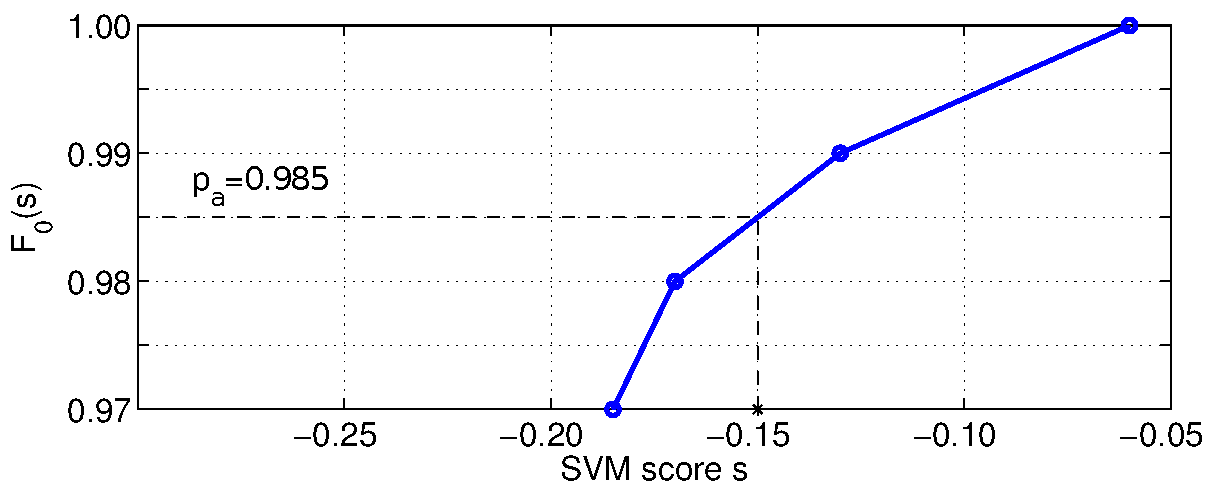
\includegraphics[width=\linewidth]{imgs/qnt1x}
            \label{fig:subfig1}
         }
         \vspace{1.5mm}\newline
         \subfigure[]{
            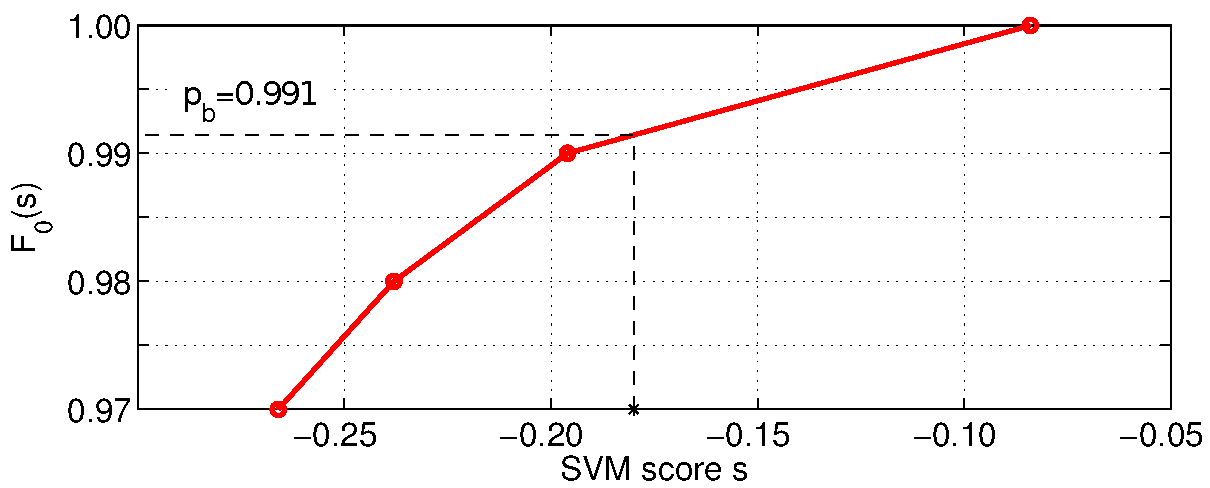
\includegraphics[width=\linewidth]{imgs/qnt2x}
            \label{fig:subfig2}
         }
         \vspace*{-3mm}
         \caption[]{
            An illustration of the proposed normalization of SVM~scores for two different database images. In each plot, the x-axis shows the raw SVM score. The y-axis shows the calibrated output. For the given query, the raw SVM score of image (b) is lower than for image (a), but the calibrated score of image (b) is higher than for image (a). 
         }
         \vspace*{-2mm}
         \label{fig:calib}
      \end{figure}
   %%%%%%%%%%%%%%%%%%%%%%%%%%%%%%%%%%%%%%%%%%%%%%%%%
   \paragraph{Summary of the calibration procedure.}
   %%%%%%%%%%%%%%%%%%%%%%%%%%%%%%%%%%%%%%%%%%%%%%%%%
      For each place, keep $\Ncal$ scores from negative examples $(s_n)_{1 \leq n \leq \Ncal}$ used for calibration together with the associated cumulative probability values $\hat{F}_0(s_n)$.
      Given the score of the query $s_q$:\\
      1.  Find $n$ such that $s_{n} \leq s_q < s_{n+1} $\\
      2.  Compute the interpolated empirical cdf value $$\hat{F}_0(s_q)\approx \hat{F}_0(s_n)+\frac{s_q-s_n}{s_{n+1}-s_n} (\hat{F}_0(s_{n+1})-\hat{F}_0(s_n)).$$
   %%%%%%%%%%%%%%%%%%%%%%%
   \paragraph{Discussion.}
   %%%%%%%%%%%%%%%%%%%%%%% 
      It should be noted that basing the calibration only on the negative data has the advantage that we privilege precision over recall, which is justified given the imbalance of the available training data (much more negatives than positives).
      Indeed, since we are learning with a single positive example, intuitively, we cannot guarantee that the learned partition of the space will generalize well to other positives, whose scores in the test set can potentially drop significantly (this is indeed what we observe in practice). By contrast, since we are learning from a comparatively large number of negative examples, we can trust the fact that new negative examples will stay in the half-space containing the negative training set, so that their scores are very unlikely to be large. Our method is therefore based on the fact that we can measure reliably how surprising a high score would be if it was the score of a negative example. This exactly means that we can control false positives (type I error) reasonably well but not false negatives (type II error or equivalently the power of our test/classifier), exactly as in the Neyman-Pearson framework.

      An additional reason for not relying on positive examples for the calibration in our case is that (even if we had sufficiently many of them) the positive examples that we collect using location and geometric verification from the geotagged database typically have illumination conditions that are extremely similar to each other and not representative of the distribution of test positives which can have very different illuminations. This is because of the controlled nature of the capturing process of geotagged street-level imagery (e.g.\ Google street-view) used for experiments in this work. Close-by images are typically captured at a similar time (e.g. on the same day) and under similar imaging conditions.



%%%%%%%%%%%%%%%%%%%%%%%
\section{Experiments}
\label{sec:experiments}
%%%%%%%%%%%%%%%%%%%%%%%
   In this section we first give implementation details, then describe the experimental datasets and finally compare performance of the proposed approach with several baseline methods.
   %%%%%%%%%%%%%%%%%%%%%%%%%%%%%%%%%%%
   \paragraph{Implementation details.}
   %%%%%%%%%%%%%%%%%%%%%%%%%%%%%%%%%%%
      All images are described using the bag-of-visual-words representation~\cite{Sivic2003}. First, SURF~\cite{Bay06} 
      %or rootSIFT~\cite{Arandjelovic12} 
      descriptors are extracted. Second, a vocabulary of 100k visual words is learnt by approximate k-means clustering~\cite{Philbin07} from a subset of features from 2,000 randomly selected images. Third, a tf-idf vector is computed for each image by assigning each descriptor to the nearest cluster center.  Finally, all tf-idf vectors are normalized to have unit $L_2$ norm.

      To learn the classifier for database image $j$, the positive and negative training data
      is constructed as follows. 
      The \emph{negative training set} $N_j$ is obtained by: (i) finding the set of images with geographical distance greater than $200{\rm m}$; (ii)  sorting the images by decreasing value of similarity to image $j$ measured by the dot product between their respective tf-idf vectors; (iii) taking the top $N=200$ ranked images as the negative set. 
      In other words, the negative training data consists of the hard negative images, i.e.\ those that are very similar to image $j$ but are far away from its geographical position, hence, cannot have the same visual content.

      The \emph{positive training set} $P_j$ initially consist of the image $j$ itself and can be expanded by:  (i) finding the adjacent images (e.g. images located within~$<20m$ of image $j$), (ii) identifying adjacent images with the same visual content using geometric verification, and (iii) adding these verified images to the positive set $P_j$.

      For SVM training we use {\tt libsvm} \cite{libsvm}. We set the value of the regularization parameters to $C_1=1 \cdot n_P$ for positive data and $C_2=10^{-3} \cdot n_N$ for negative data where $n_P$ and $n_N$ denote the number of examples in the positive and the negative set, respectively. These parameters were found by cross-validation and work well on various datasets. 

      The calibration with significance levels is done for each classifier in turn as follows: (i) given image $j$ and learnt SVM we construct a set of images consisting of the whole database without the positive set $P_j$; (ii) for this image set, SVM scores are computed; (iii) empirical cdf $\hat{F}_0$ is estimated from sorted SVM scores.

      To use a reasonable amount of memory, for each classifier, we store only the first 1000 largest negative scores (the number of negative scores stored could be reduced further using interpolation).
   %%%%%%%%%%%%%%%%%%%%%%%%%%
   \paragraph{Image dataset.}
   %%%%%%%%%%%%%%%%%%%%%%%%%%
      We performed experiments on a database of Google Streetview images from the Internet. We downloaded panoramas from Pittsburgh (U.S.) covering roughly an area of $1.3 \times 1.2 \; {\rm km}^2$. Similar to~\cite{Chen11}, we generate for each panorama 12 overlapping perspective views corresponding to two different elevation angles to capture both the street-level scene and the building fa\c{c}ades, resulting in a total of 24 perspective views each with $90^\circ$ FOV and resolution of $960 \times 720$ pixels. This dataset contains 25,000 perspective images.

      As a query set with known ground truth GPS positions, we use the 8999 panoramas from the Google Streetview research dataset, which cover approximately the same area, but were captured at a different time, and typically depict the same places from different viewpoints and under different illumination conditions. For each test panorama, we generate perspective images as described above. Finally, we randomly select out of all generated perspective views a subset of 4k images, which is used as a test set to evaluate the performance of the proposed approach.

   %%%%%%%%%%%%%%%%%%%%
   \paragraph{Results.}
   %%%%%%%%%%%%%%%%%%%%
      We compare the performance of the proposed approach (SVM p-val) with the following baseline methods: (a) Training per-location classifiers without any calibration step (SVM). (b) Calibrating per-location classifiers using the standard logistic regression\footnote
         {
         The calibration of SVM scores with logistic regression is based on a subset of 30 hard negatives from $N_j$ and 1-15 available positive examples from $P_j$.
         } 
      as in exemplar SVM~\cite{Malisiewicz11} (SVM logistic). (c) The standard bag-of-visual words retrieval (BOW)~\cite{Philbin07}. (d) Our implementation of the confuser suppression  approach (Conf. supp.) of~\cite{Knopp2010} that, in each database image, detects and removes features that frequently appear at other far-away locations (using parameters $t=3.5$ and $w=70$).

      For all methods, we implemented a two-stage place recognition approach. Given a query image, the aim of the first stage is to efficiently find a small subset (20) of candidates that are likely to depict the same place as the query image. In the second stage, we search for restricted homographies between candidates and the query image using RANSAC~\cite{Philbin07}. The candidates are finally re-ranked by decreasing number of inliers.

      \begin{table}[t]
         \begin{center}
            \begin{tabularx}{\linewidth}{l c c}
               \hline
               \rowcolor{lightgray}
               Method \hspace{47pt}      & $\%$ correct          &   $\%$ correct \\
               \rowcolor{lightgray}
                          & {\it init. retrieval} &  {\it with geom. verif.} \\
               \hline \hline
               SVM                          & $00.0$     & $12.7 $      \\
               SVM logistic                 & $03.6$     & $10.3$       \\
               BOW                          & $32.0$     & $53.1$       \\
               Conf. supp.~\cite{Knopp2010} & $36.5$     & $58.1$       \\
               {\bf SVM p-val}              & $\bf 41.9$ & $\bf 60.8$   \\
               \hline
            \end{tabularx}
            \vspace*{-2mm}
            \caption{
            The percentage of correctly localized test queries for which the top-ranked database image is within $20$ meters from the ground truth query position. The proposed method (SVM p-val) outperforms the baseline methods. Results are shown for the initial retrieval (left column) and after re-ranking the top 20 retrieved images using geometric verification. Notice that SVM output without calibration gives $0\%$ of correctly localized queries.
            }
            \label{tab:eval}
         \end{center}
         \vspace*{-6mm}
      \end{table}

      Since the ground truth GPS position for each query image is available, we measure the overall recognition performance by the percentage of query test images for which the top-ranked database image was located within a distance of $20$ meters from the ground truth query location.  Results are summarized in table~\ref{tab:eval} and clearly demonstrate the benefits of  careful calibration of the per-location classifiers. In addition, the proposed per-location classifier method outperforms the baseline bag-of-visual-word approach~\cite{Philbin07} including confuser suppression~\cite{Knopp2010}.

      Examples of correctly and incorrectly localized queries are shown in figure~\ref{fig:demo1}. Figure~\ref{fig:3qVSw} illustrates the weights learnt for one database image applied
      to three different query images.

   %%%%%%%%%%%%%%%%%%%%%%%%
   \paragraph{Scalability.}
   %%%%%%%%%%%%%%%%%%%%%%%% 
      The linear SVM classifiers trained for each database image are currently non-sparse,
      which increases the computational and memory requirements
      at query time compared to the original bag-of-visual-words representation.
      For a database of 25,000 images, applying all classifiers on a query image takes currently on average 1.72s. The method could be further sped-up by, for example: (i) reducing the dimensionality of the input vectors~\cite{Jegou12}, or (ii) enforcing additional sparsity constraints on learnt weight vectors $w$.

   \begin{figure*}[!ht]
	 \begin{minipage}{0.23\linewidth}
		\centering
		Query image
	 \end{minipage}
	 \hspace{3mm}
	 \begin{minipage}{0.23\linewidth}
		\centering
		Per-location class.
	 \end{minipage}
	 \begin{minipage}{0.23\linewidth}
		\centering
		Confuser suppression
	 \end{minipage}
	 \begin{minipage}{0.23\linewidth}
		\centering
		Bag-of-words
	 \end{minipage}
  \\
	 \colorbox{gray}{
		\begin{minipage}{\subw}
		  \centerline{
		  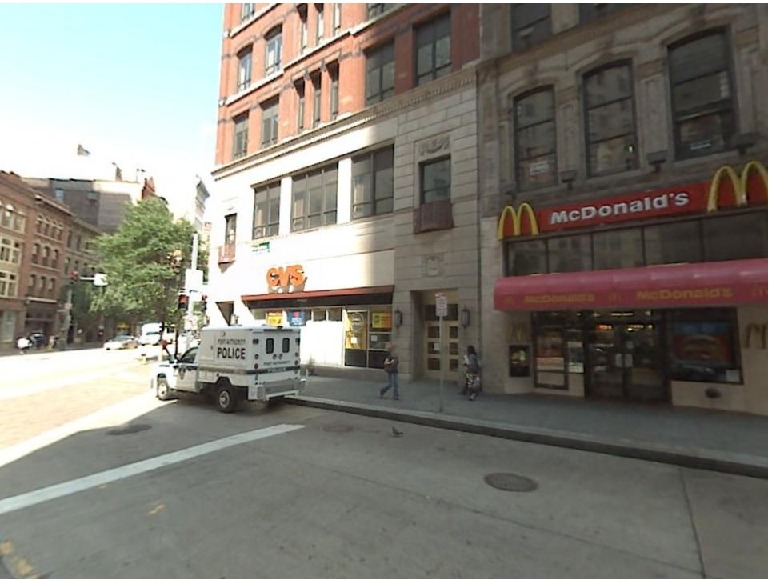
\includegraphics[width=1.05\linewidth]{imgs/demo01d.pdf}
		  }
		\end{minipage}
	 }
	 \hspace{3mm}
	 %%%%%%%%%%
	 %
	 \colorbox{myGreen}{
		\begin{minipage}{\subw}
		  \centerline{
		  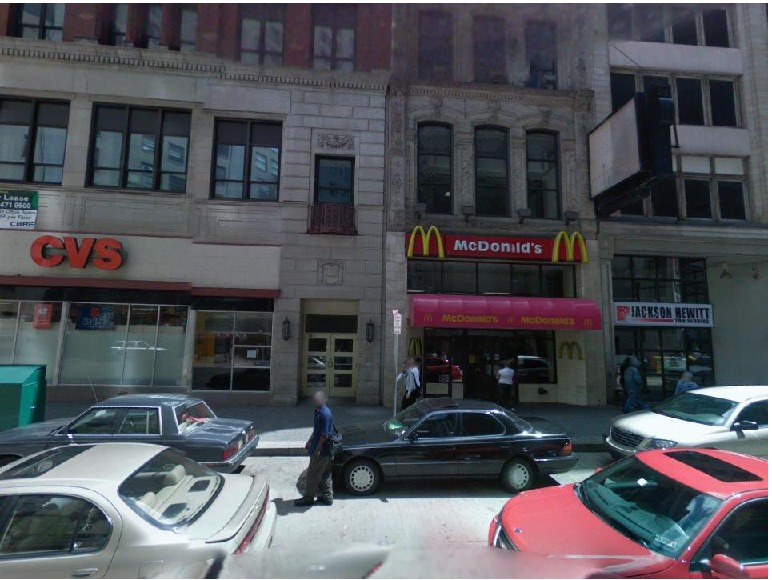
\includegraphics[width=1.05\linewidth]{imgs/demo02d.pdf}
		  }
		\end{minipage}
	 }
	 %
	 \colorbox{myRed}{
		\begin{minipage}{\subw}
		  \centerline{
		  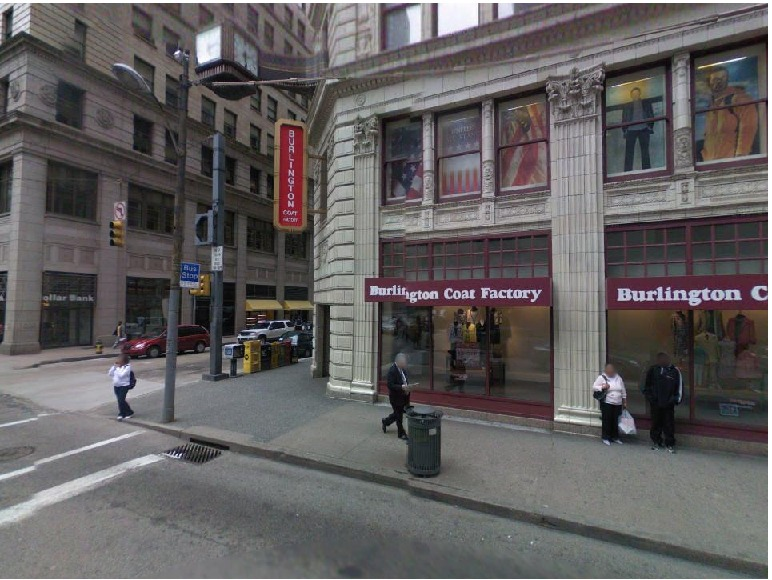
\includegraphics[width=1.05\linewidth]{imgs/demo03d.pdf}
		  }
		\end{minipage}
	 }
	 %
	 \colorbox{myRed}{
		\begin{minipage}{\subw}
		  \centerline{
		  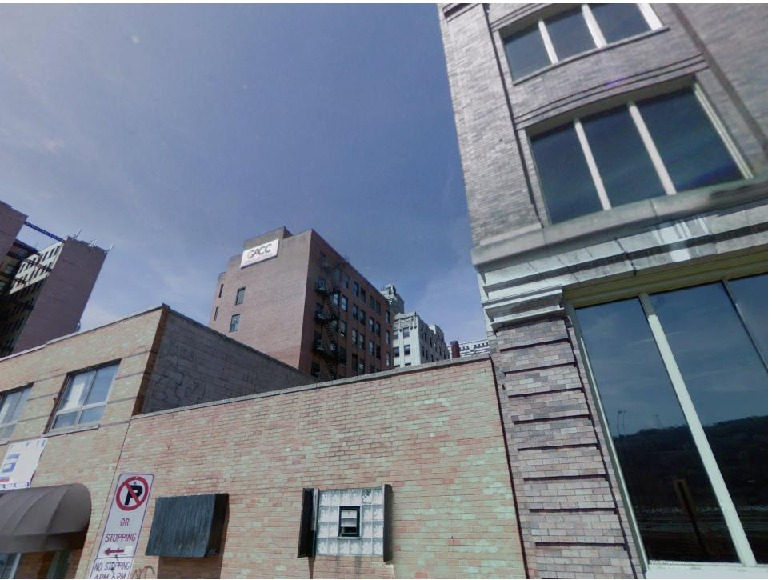
\includegraphics[width=1.05\linewidth]{imgs/demo04d.pdf}
		  }
		\end{minipage}
	 }
	 \vspace{1mm}
	 %%%%%%%%%%%%%%%%%%%%%%%%%%%%%%%%%%%%%%%%%%%%%%%%%%%%%%%%%%%%%%%%%%%%%%%
	 \\
	 \colorbox{gray}{
		\begin{minipage}{\subw}
		  \centerline{
		  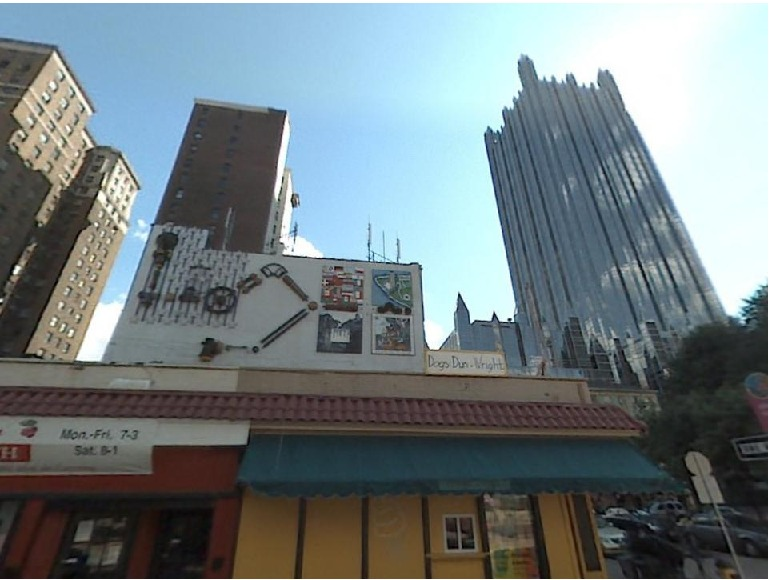
\includegraphics[width=1.05\linewidth]{imgs/demo01.pdf}
		  }
		\end{minipage}
	 }
	 \hspace{3mm}
	 %%%%%%%%%
	 %
	 \colorbox{myGreen}{
		\begin{minipage}{\subw}
		  \centerline{
		  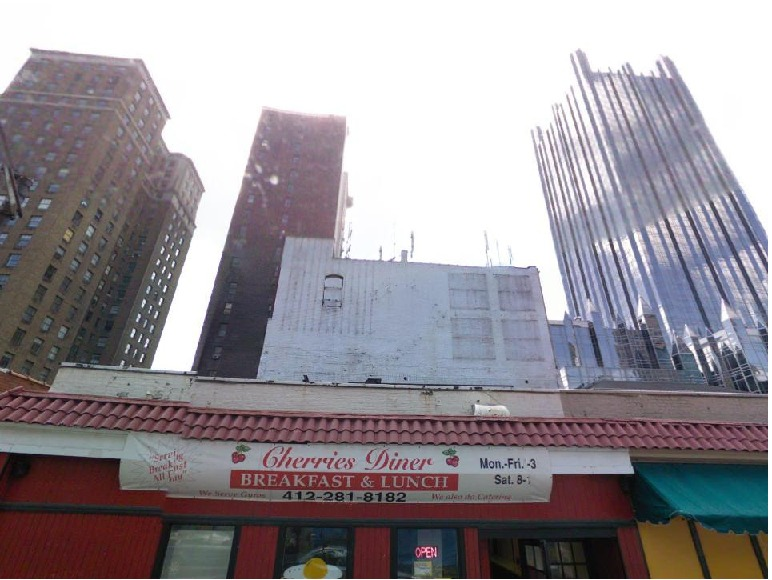
\includegraphics[width=1.05\linewidth]{imgs/demo02.pdf}
		  }
		\end{minipage}
	 }
	 %
	 \colorbox{myRed}{
		\begin{minipage}{\subw}
		  \centerline{
		  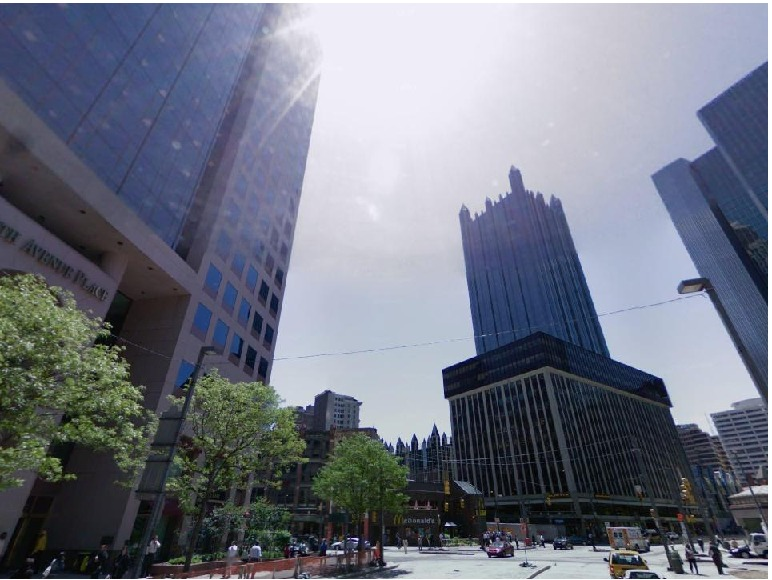
\includegraphics[width=1.05\linewidth]{imgs/demo03.pdf}
		  }
		\end{minipage}
	 }
	 %
	 \colorbox{myRed}{
		\begin{minipage}{\subw}
		  \centerline{
		  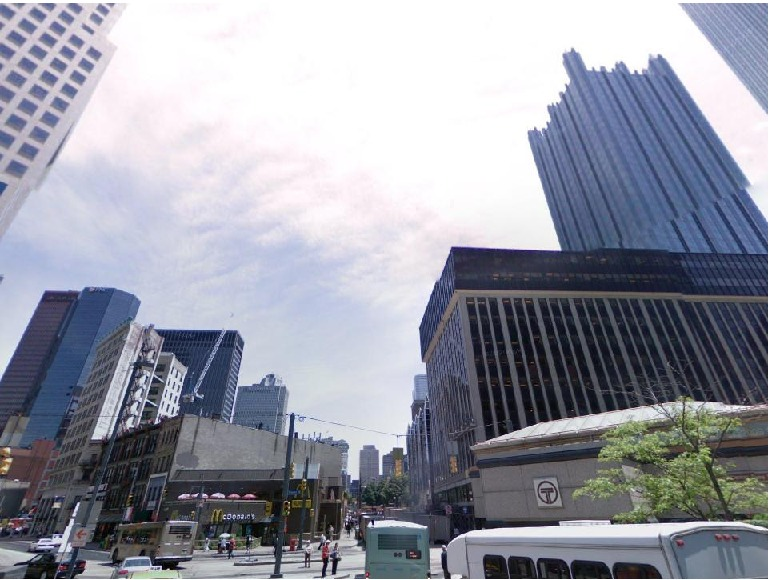
\includegraphics[width=1.05\linewidth]{imgs/demo04.pdf}
		  }
		\end{minipage}
	 }
	 \vspace{1mm}
	 %%%%%%%%%%%%%%%%%%%%%%%%%%%%%%%%%%%%%%%%%%%%%%%%%%%%%%%%%%%%%%%%%%%%%%%
	 \\
	 \colorbox{gray}{
		\begin{minipage}{\subw}
		  \centerline{
		  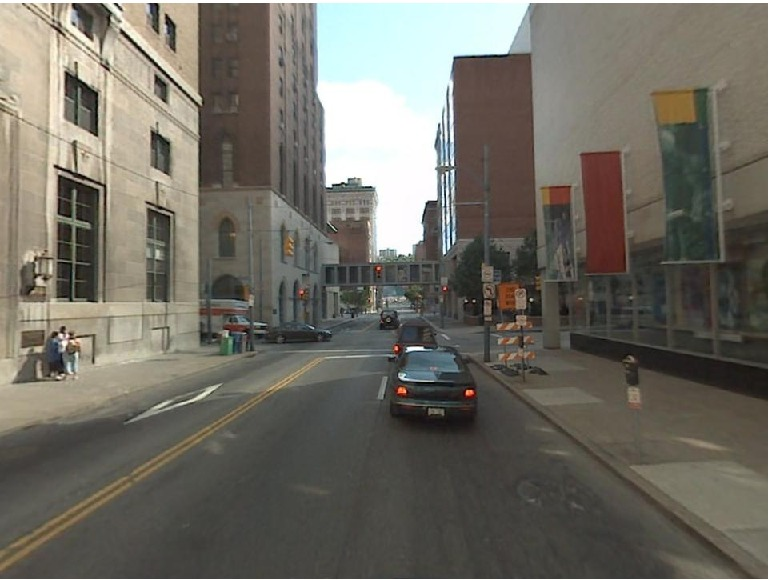
\includegraphics[width=1.05\linewidth]{imgs/demo01b.pdf}
		  }
		\end{minipage}
	 }
	 \hspace{3mm}
	 %%%%%%%%%
	 %
	 \colorbox{myGreen}{
		\begin{minipage}{\subw}
		  \centerline{
		  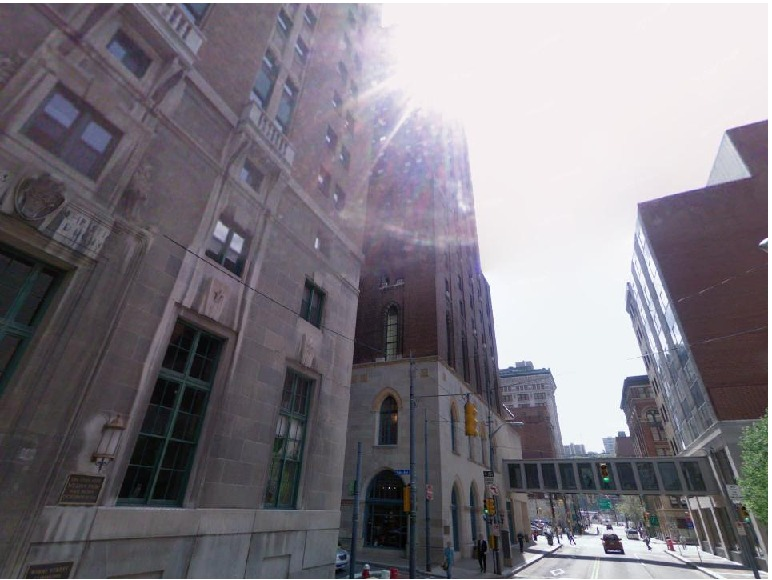
\includegraphics[width=1.05\linewidth]{imgs/demo02b.pdf}
		  }
		\end{minipage}
	 }
	 %
	 \colorbox{myRed}{
		\begin{minipage}{\subw}
		  \centerline{
		  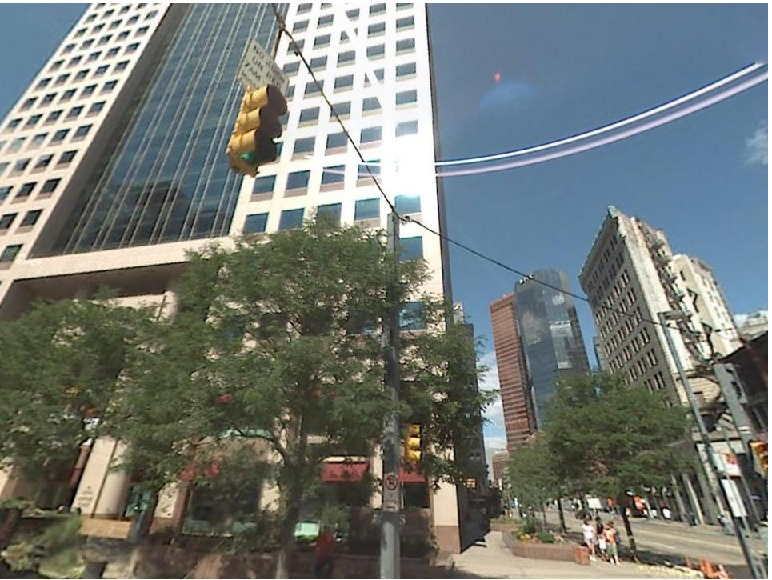
\includegraphics[width=1.05\linewidth]{imgs/demo03b.pdf}
		  }
		\end{minipage}
	 }
	 %
	 \colorbox{myRed}{
		\begin{minipage}{\subw}
		  \centerline{
		  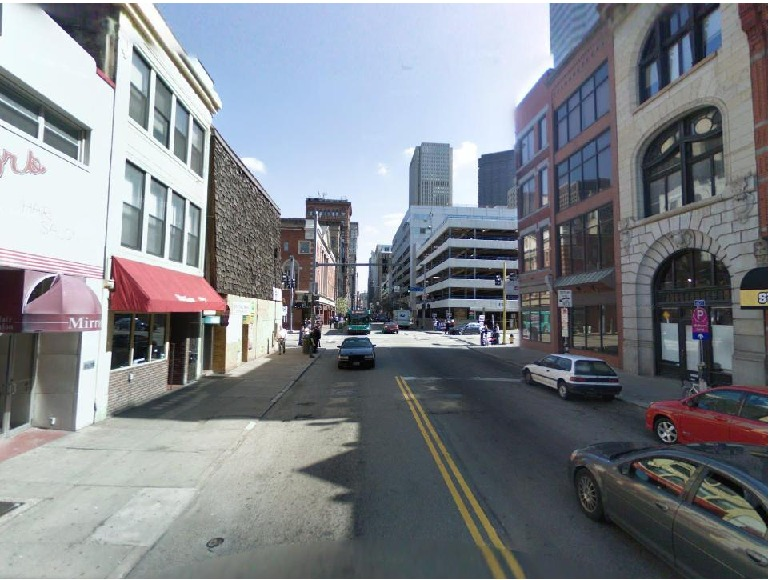
\includegraphics[width=1.05\linewidth]{imgs/demo04b.pdf}
		  }
		\end{minipage}
	 }
	 \vspace{1mm}
	 %%%%%%%%%%%%%%%%%%%%%%%%%%%%%%%%%%%%%%%%%%%%%%%%%%%%%%%%%%%%%%%%%%%%%%%
	 \\
	 \colorbox{gray}{
		\begin{minipage}{\subw}
		  \centerline{
		  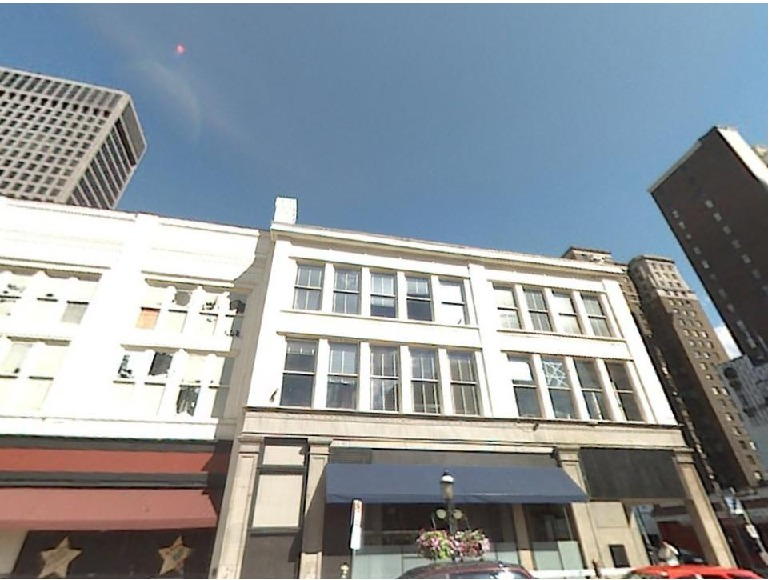
\includegraphics[width=1.05\linewidth]{imgs/demo01c.pdf}
		  }
		\end{minipage}
	 }
	 \hspace{3mm}
	 %%%%%%%%%
	 %
	 \colorbox{myGreen}{
		\begin{minipage}{\subw}
		  \centerline{
		  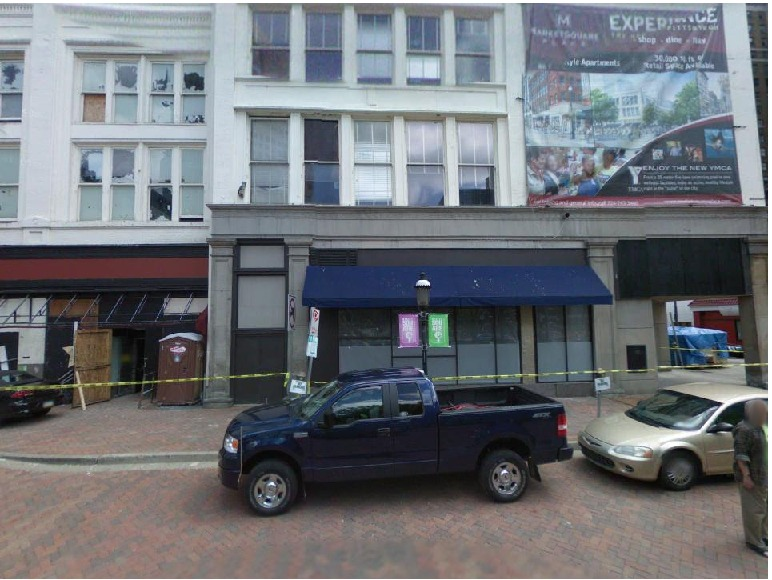
\includegraphics[width=1.05\linewidth]{imgs/demo02c.pdf}
		  }
		\end{minipage}
	 }
	 %
	 \colorbox{myRed}{
		\begin{minipage}{\subw}
		  \centerline{
		  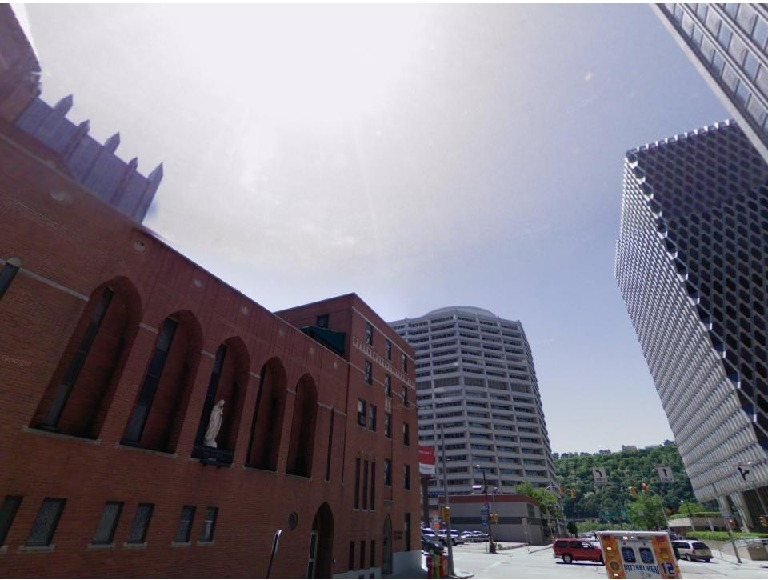
\includegraphics[width=1.05\linewidth]{imgs/demo03c.pdf}
		  }
		\end{minipage}
	 }
	 %
	 \colorbox{myRed}{
		\begin{minipage}{\subw}
		  \centerline{
		  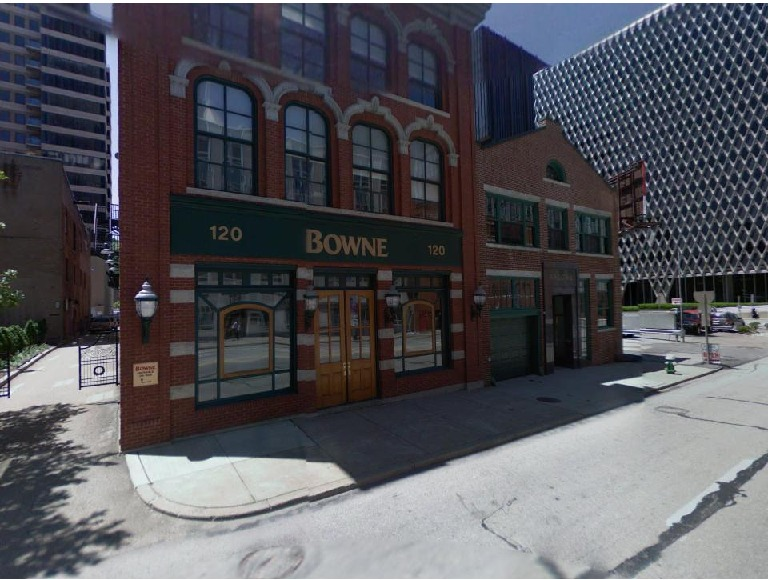
\includegraphics[width=1.05\linewidth]{imgs/demo04c.pdf}
		  }
		\end{minipage}
	 }
	 % HORIZONTAL LINE %
	 \\
	 \begin{minipage}{0.93\linewidth}
		\centering
		\begin{tabular}{c}
		  \vspace{-3mm}
		  \hspace{\linewidth} \\
		  \hline
		  \vspace{-3mm}
		\end{tabular}
	 \end{minipage}
	 %%%%%%%%%%%%%%%%%%%%%%%%%%%%%%%%%%%%%%%%%%%%%%%%%%%%%%%%%%%%%%%%%%%%%%%
	 \\
	 \colorbox{gray}{
		\begin{minipage}{\subw}
		  \centerline{
		  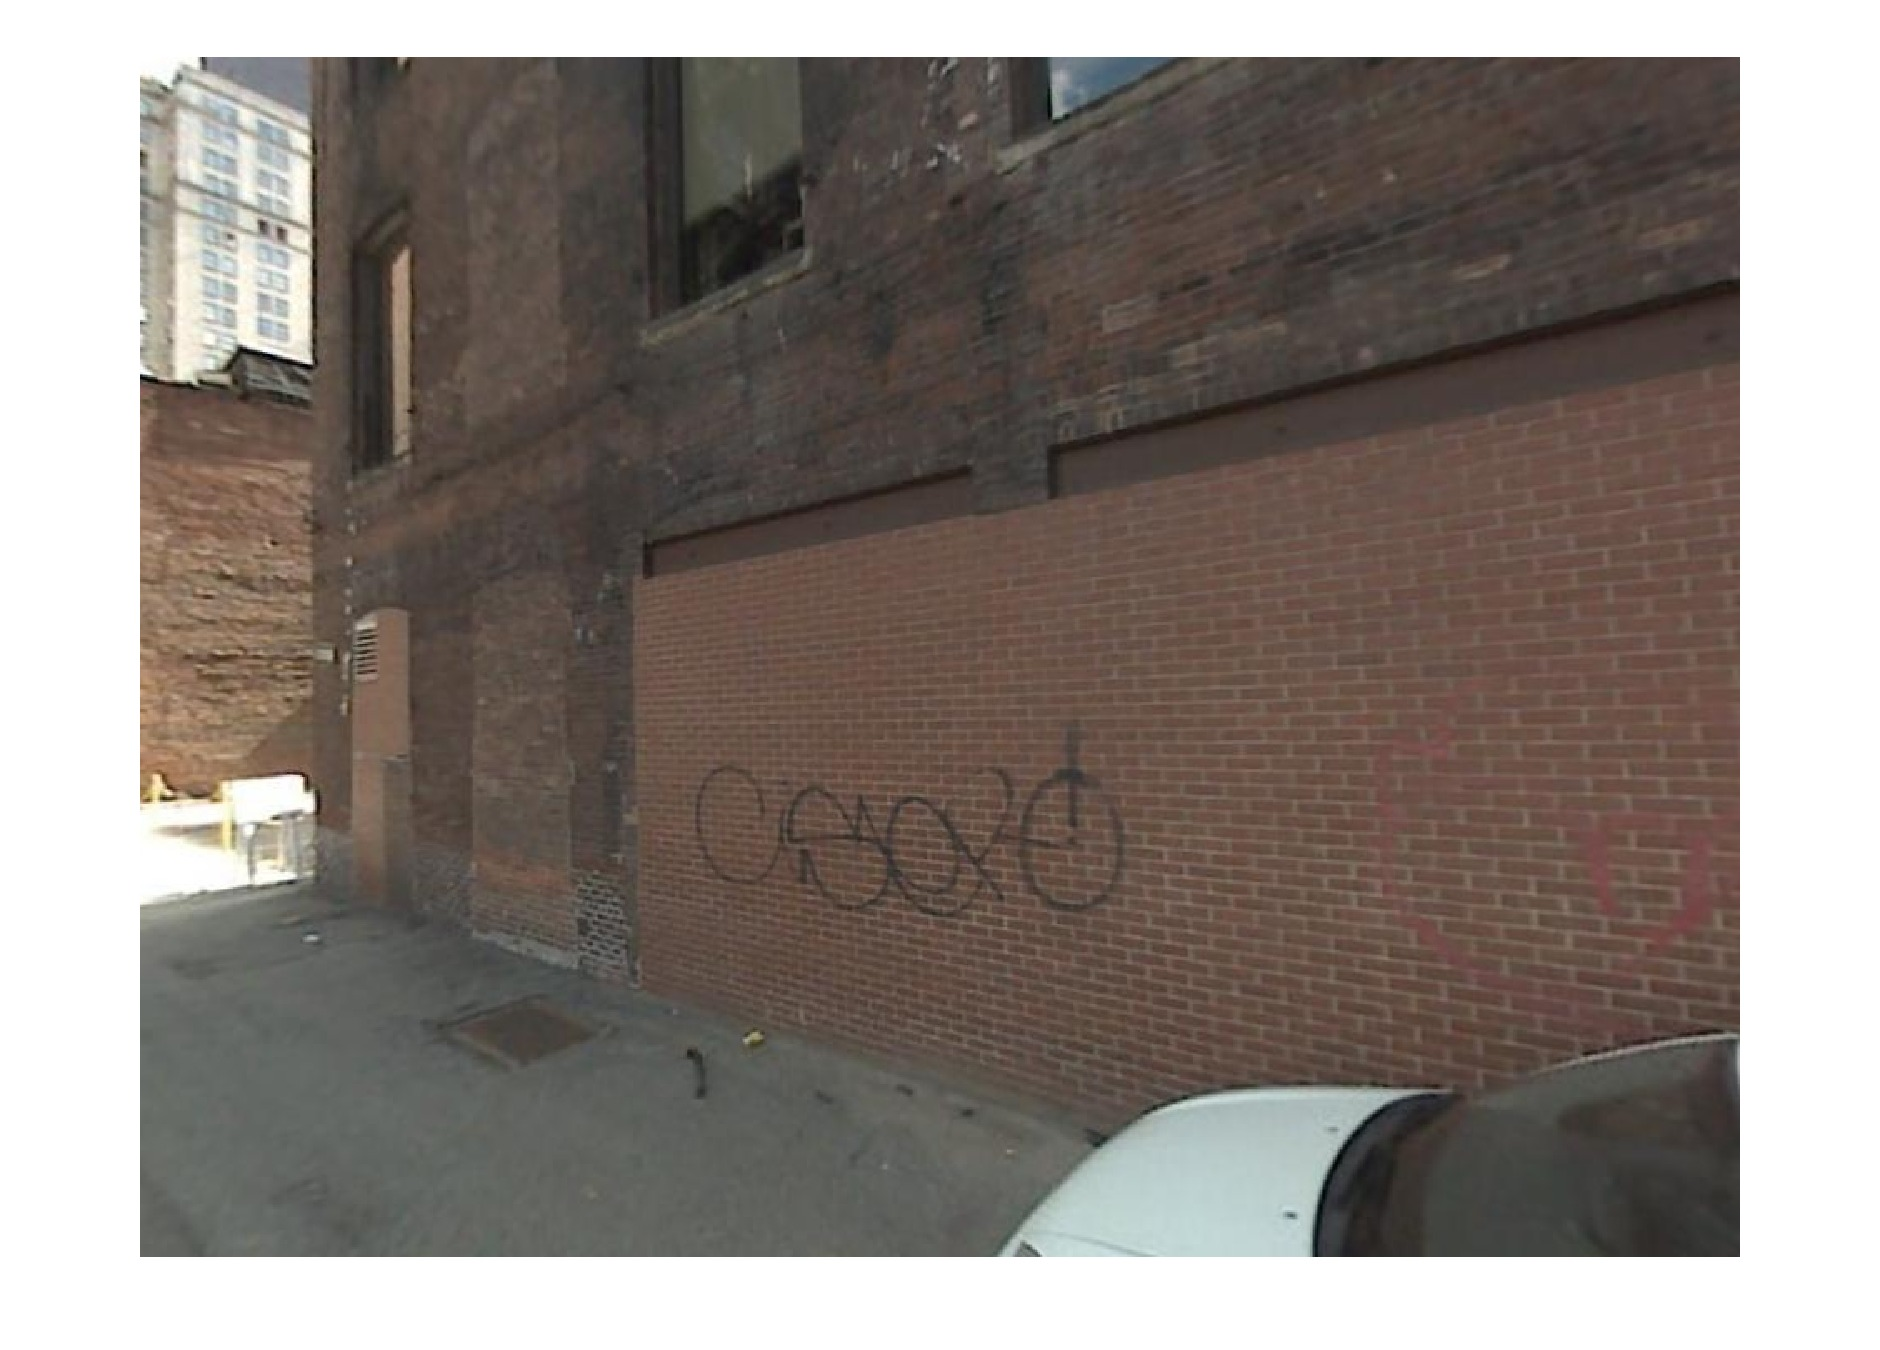
\includegraphics[width=1.05\linewidth]{imgs/aggrv/05aggrvQ.pdf}
		  }
		\end{minipage}
	 }
	 \hspace{3mm}
	 %%%%%%%%%
	 %
	 \colorbox{myRed}{
		\begin{minipage}{\subw}
		  \centerline{
		  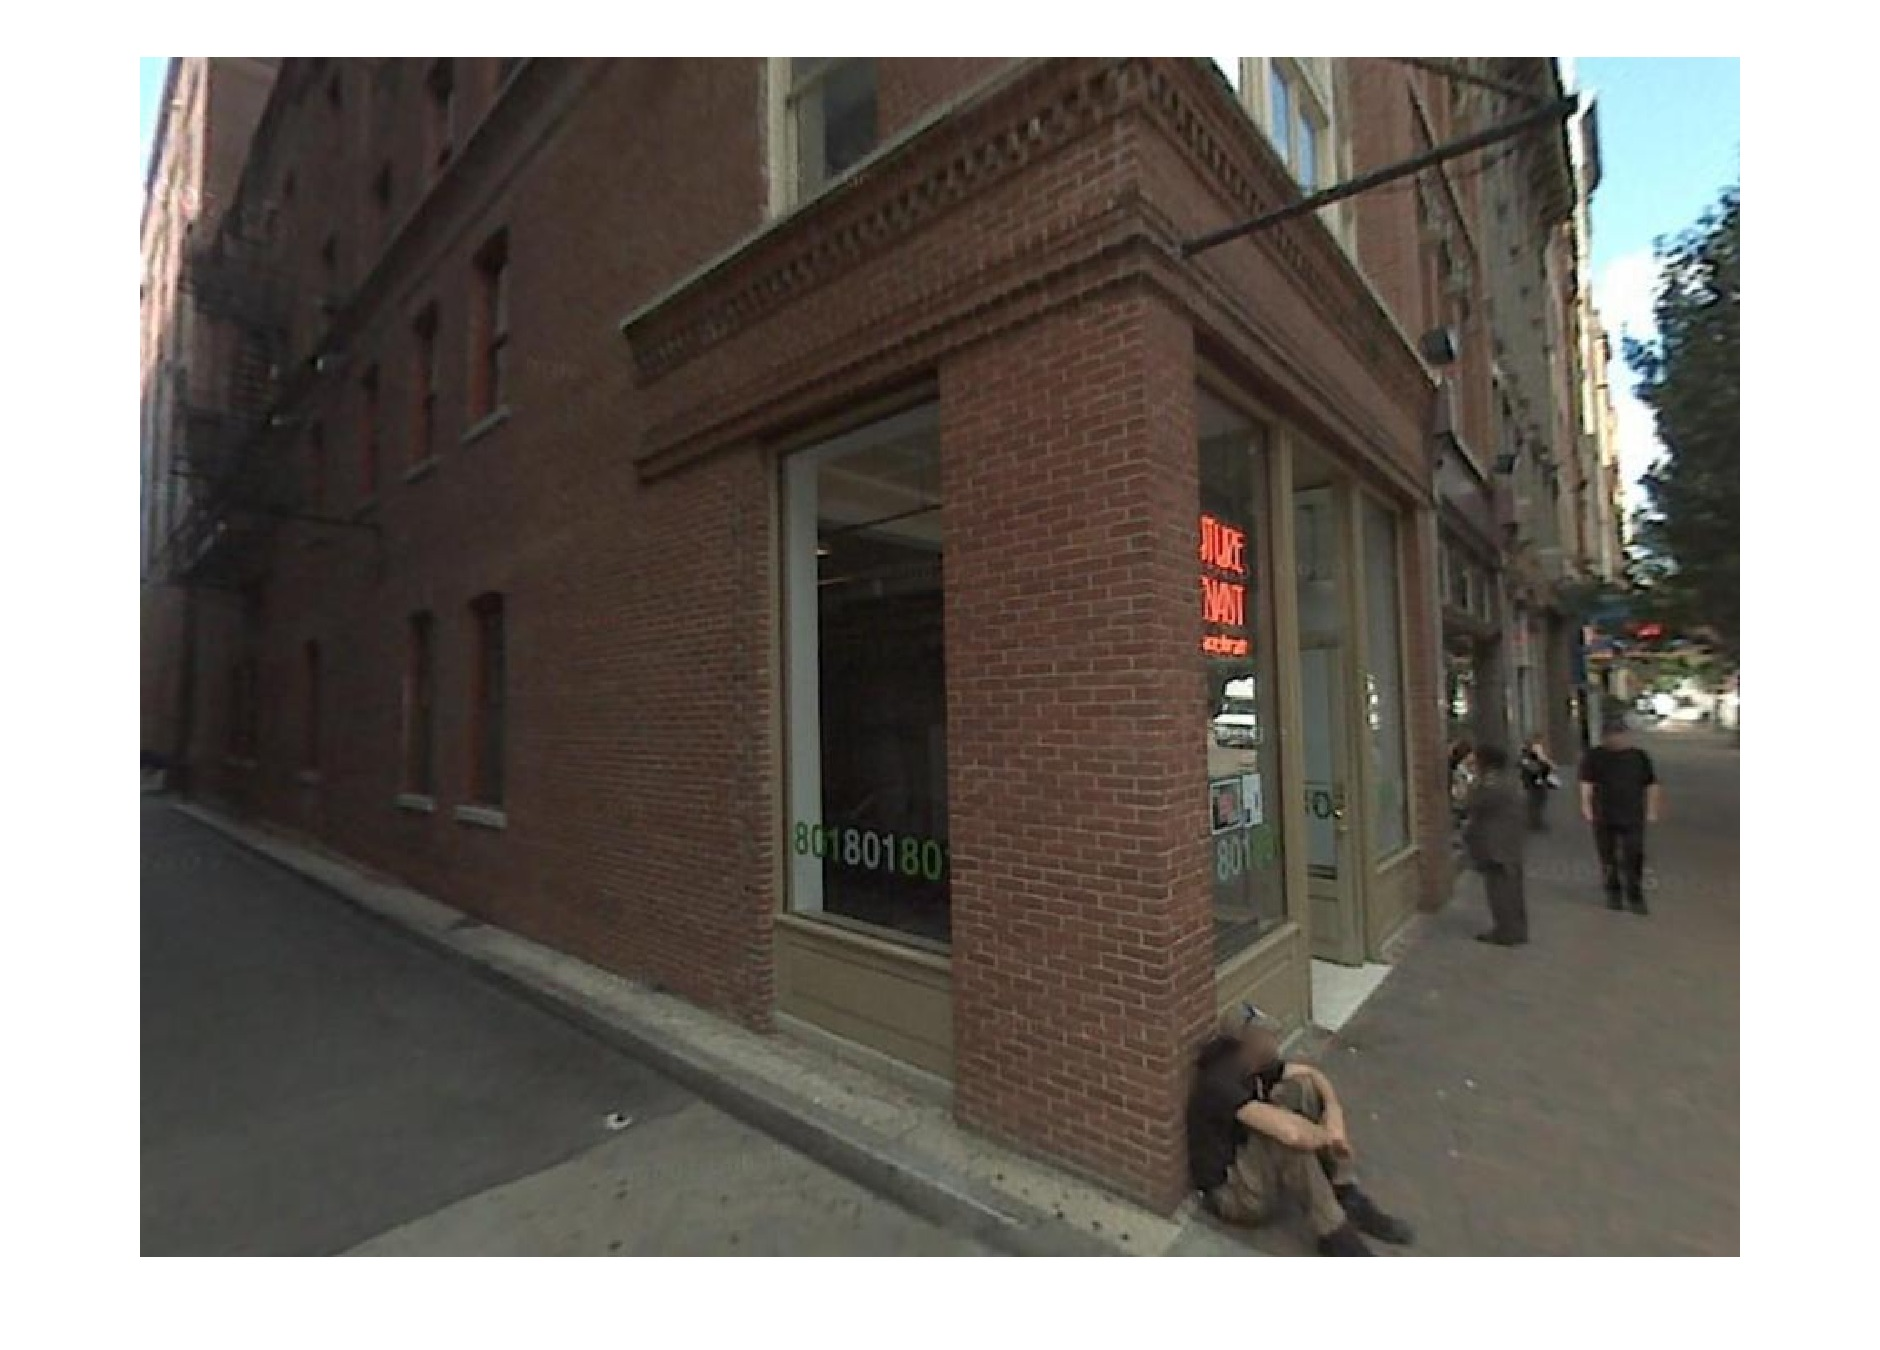
\includegraphics[width=1.05\linewidth]{imgs/aggrv/05aggrvS.pdf}
		  }
		\end{minipage}
	 }
	 %
	 \colorbox{myGreen}{
		\begin{minipage}{\subw}
		  \centerline{
		  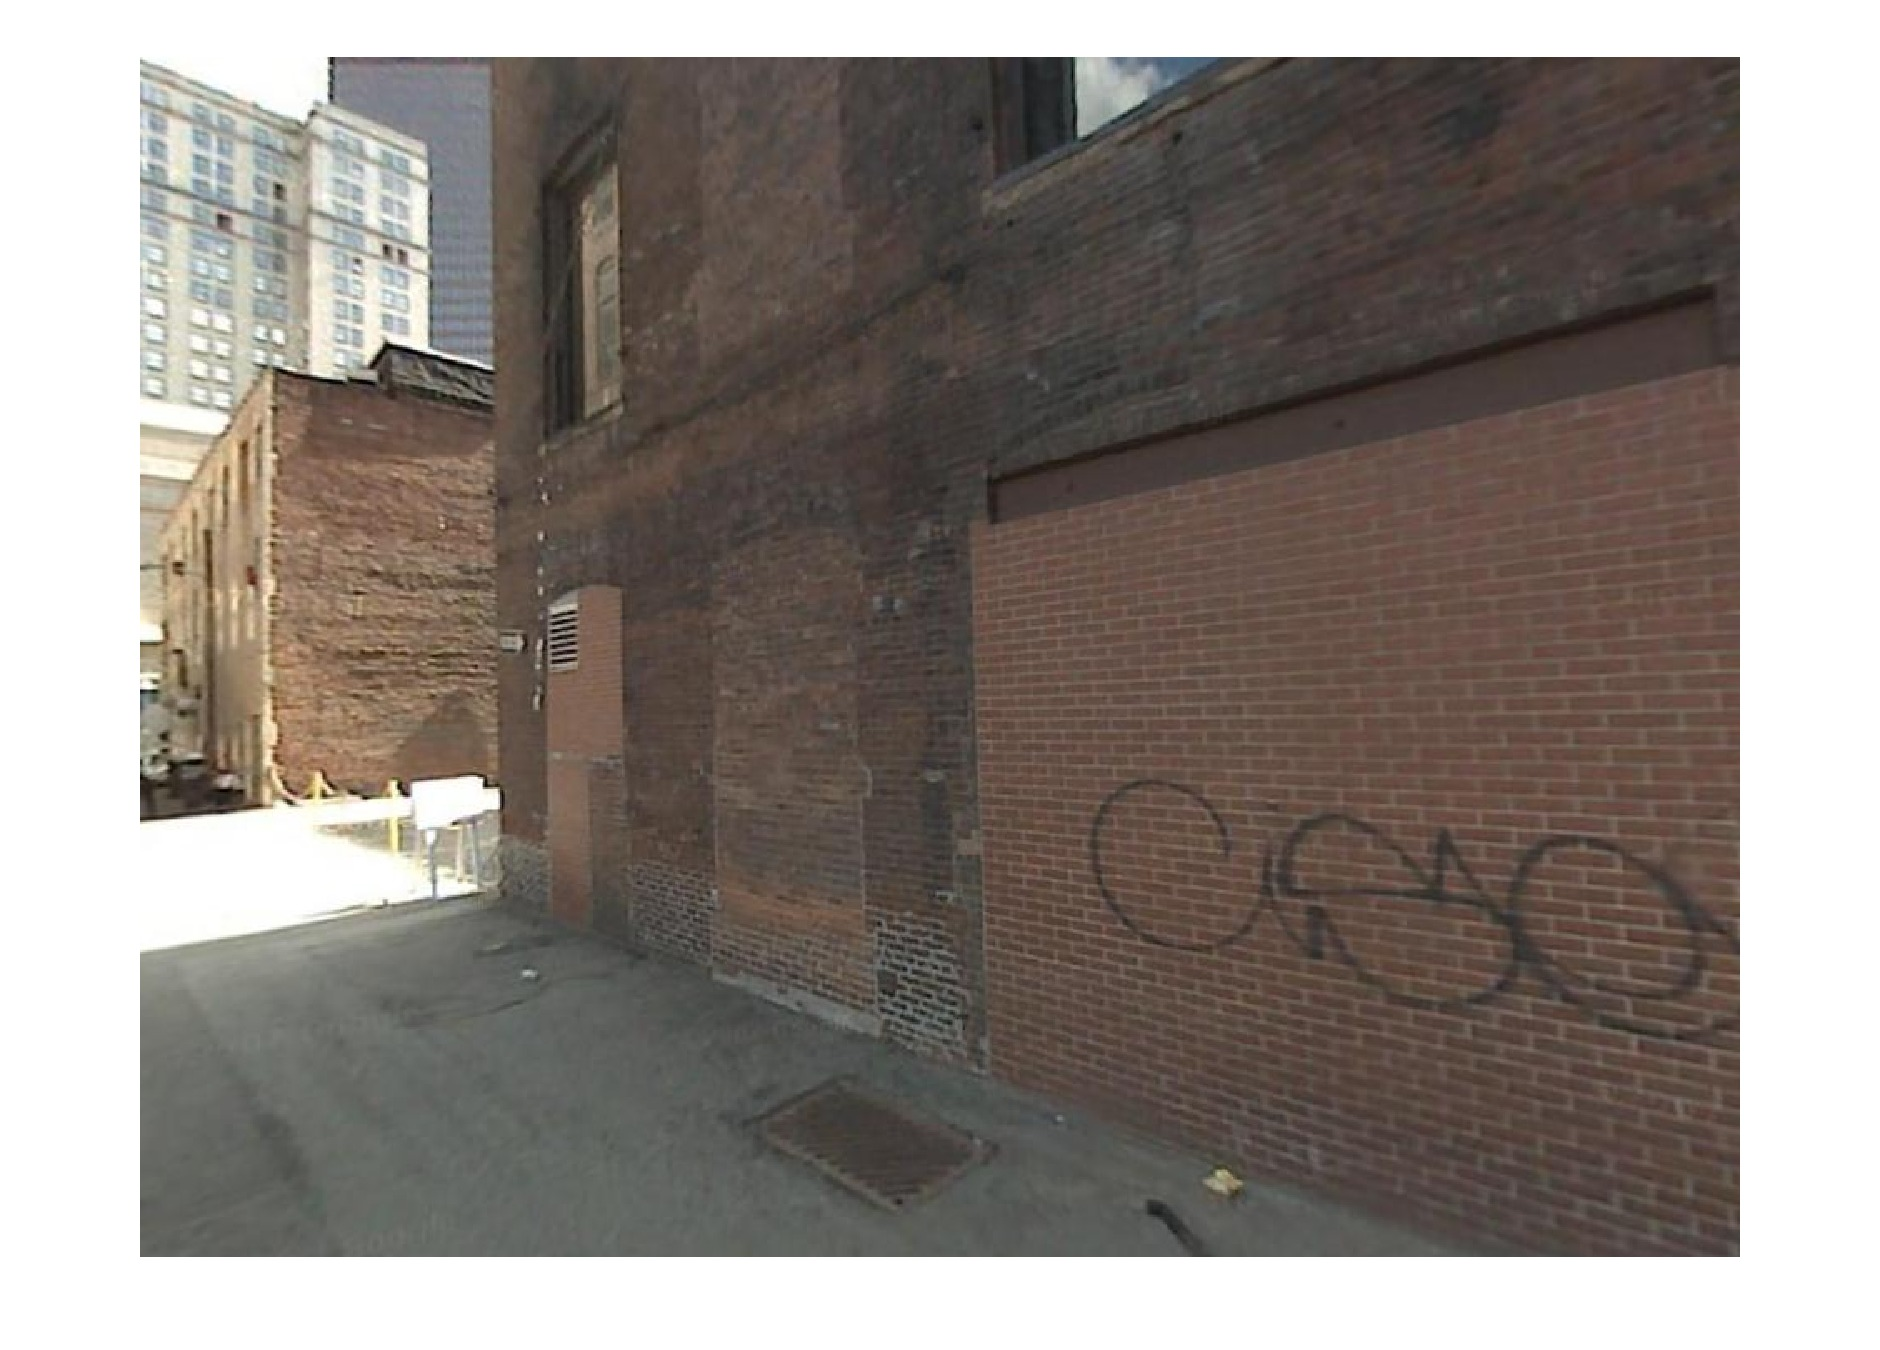
\includegraphics[width=1.05\linewidth]{imgs/aggrv/05aggrvK.pdf}
		  }
		\end{minipage}
	 }
	 %
	 \colorbox{myGreen}{
		\begin{minipage}{\subw}
		  \centerline{
		  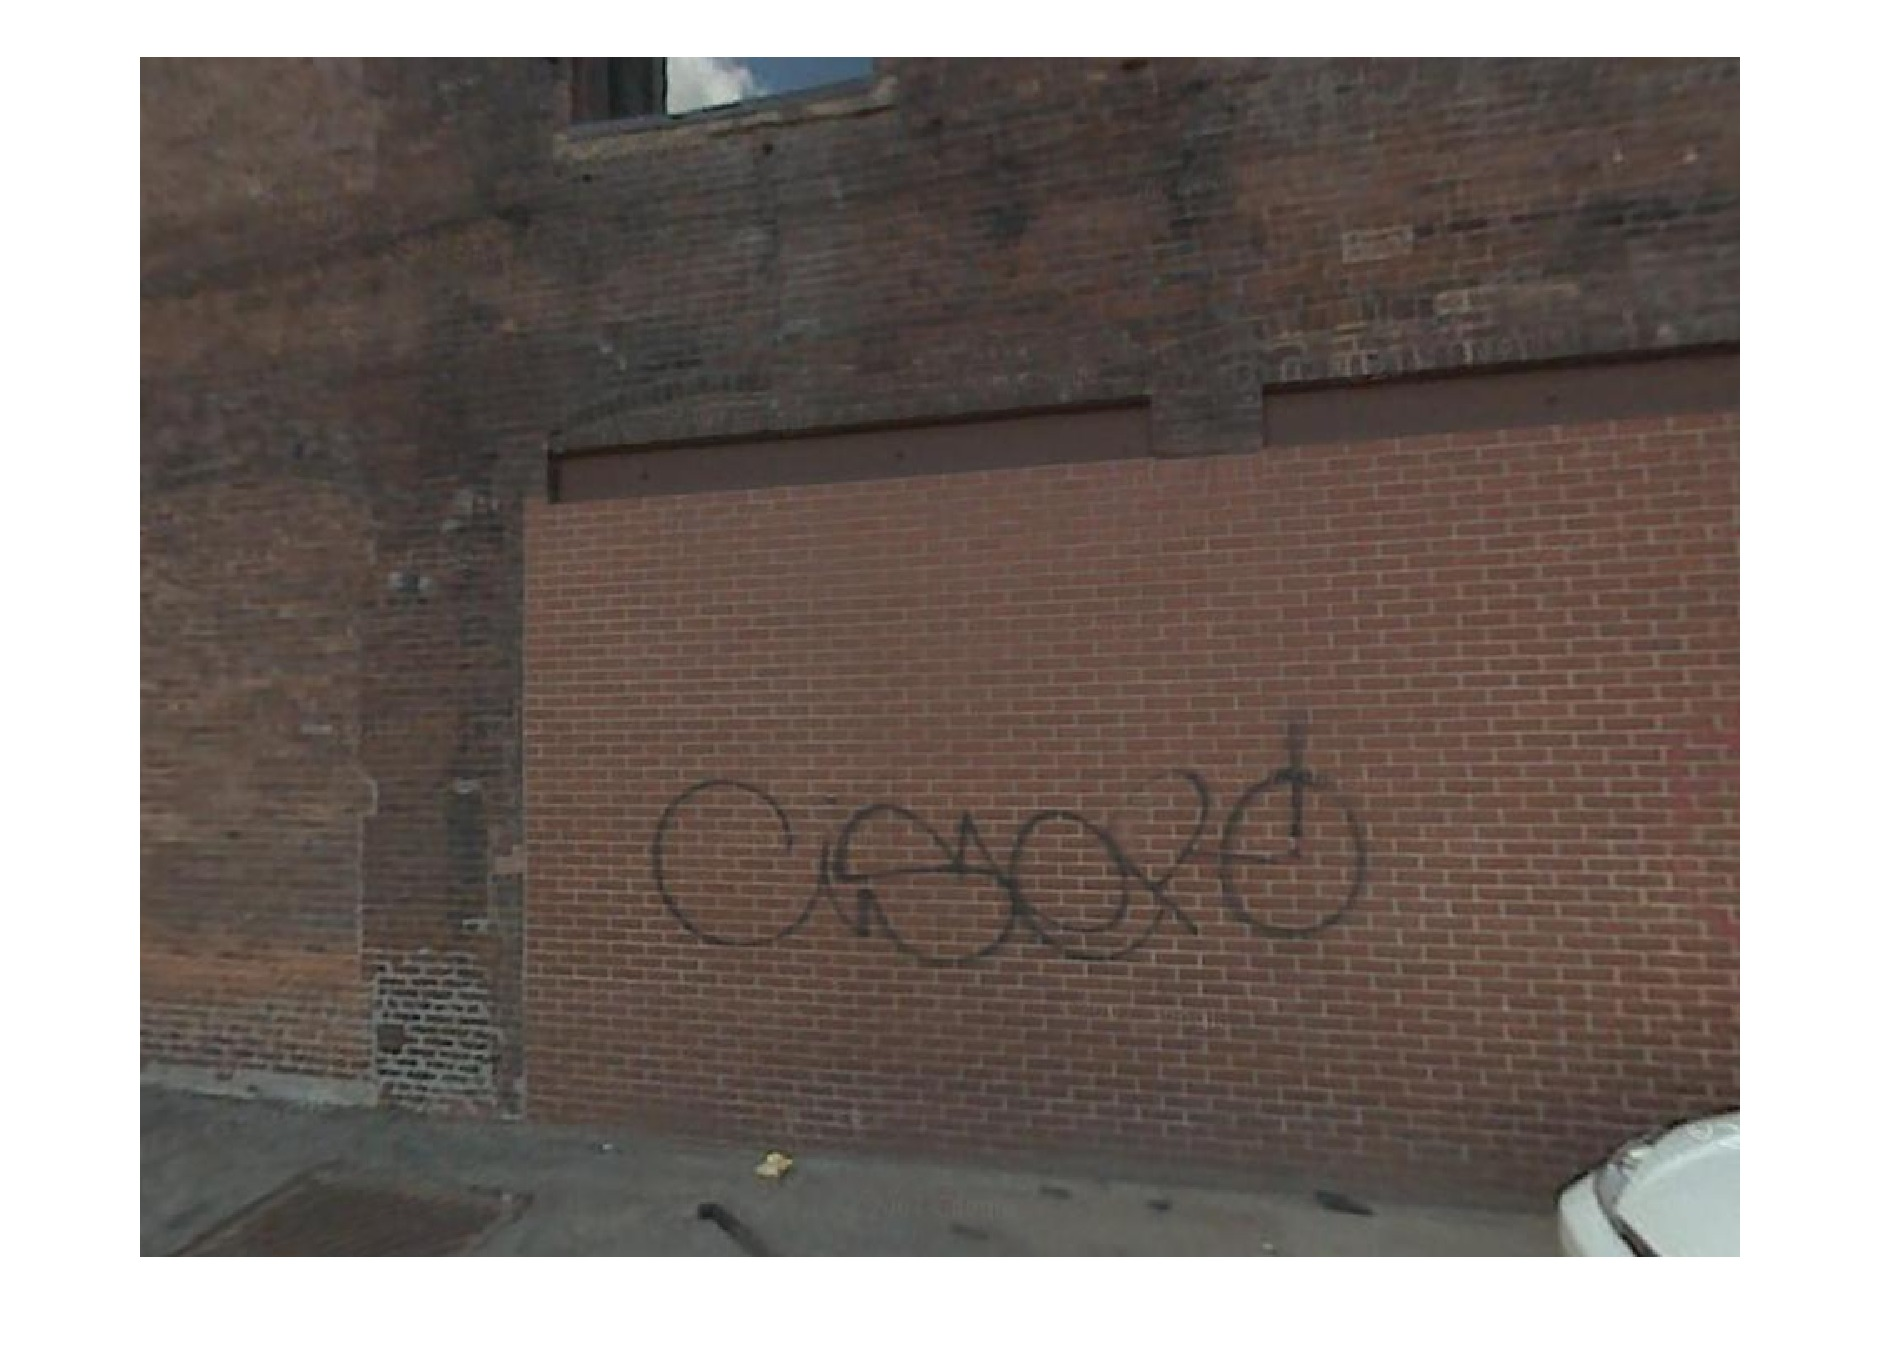
\includegraphics[width=1.05\linewidth]{imgs/aggrv/05aggrvB.pdf}
		  }
		\end{minipage}
	 }
	 \vspace{1mm}
	 %%%%%%%%%%%%%%%%%%%%%%%%%%%%%%%%%%%%%%%%%%%%%%%%%%%%%%%%%%%%%%%%%%%%%%%
	 \\
	 \colorbox{gray}{
		\begin{minipage}{\subw}
		  \centerline{
		  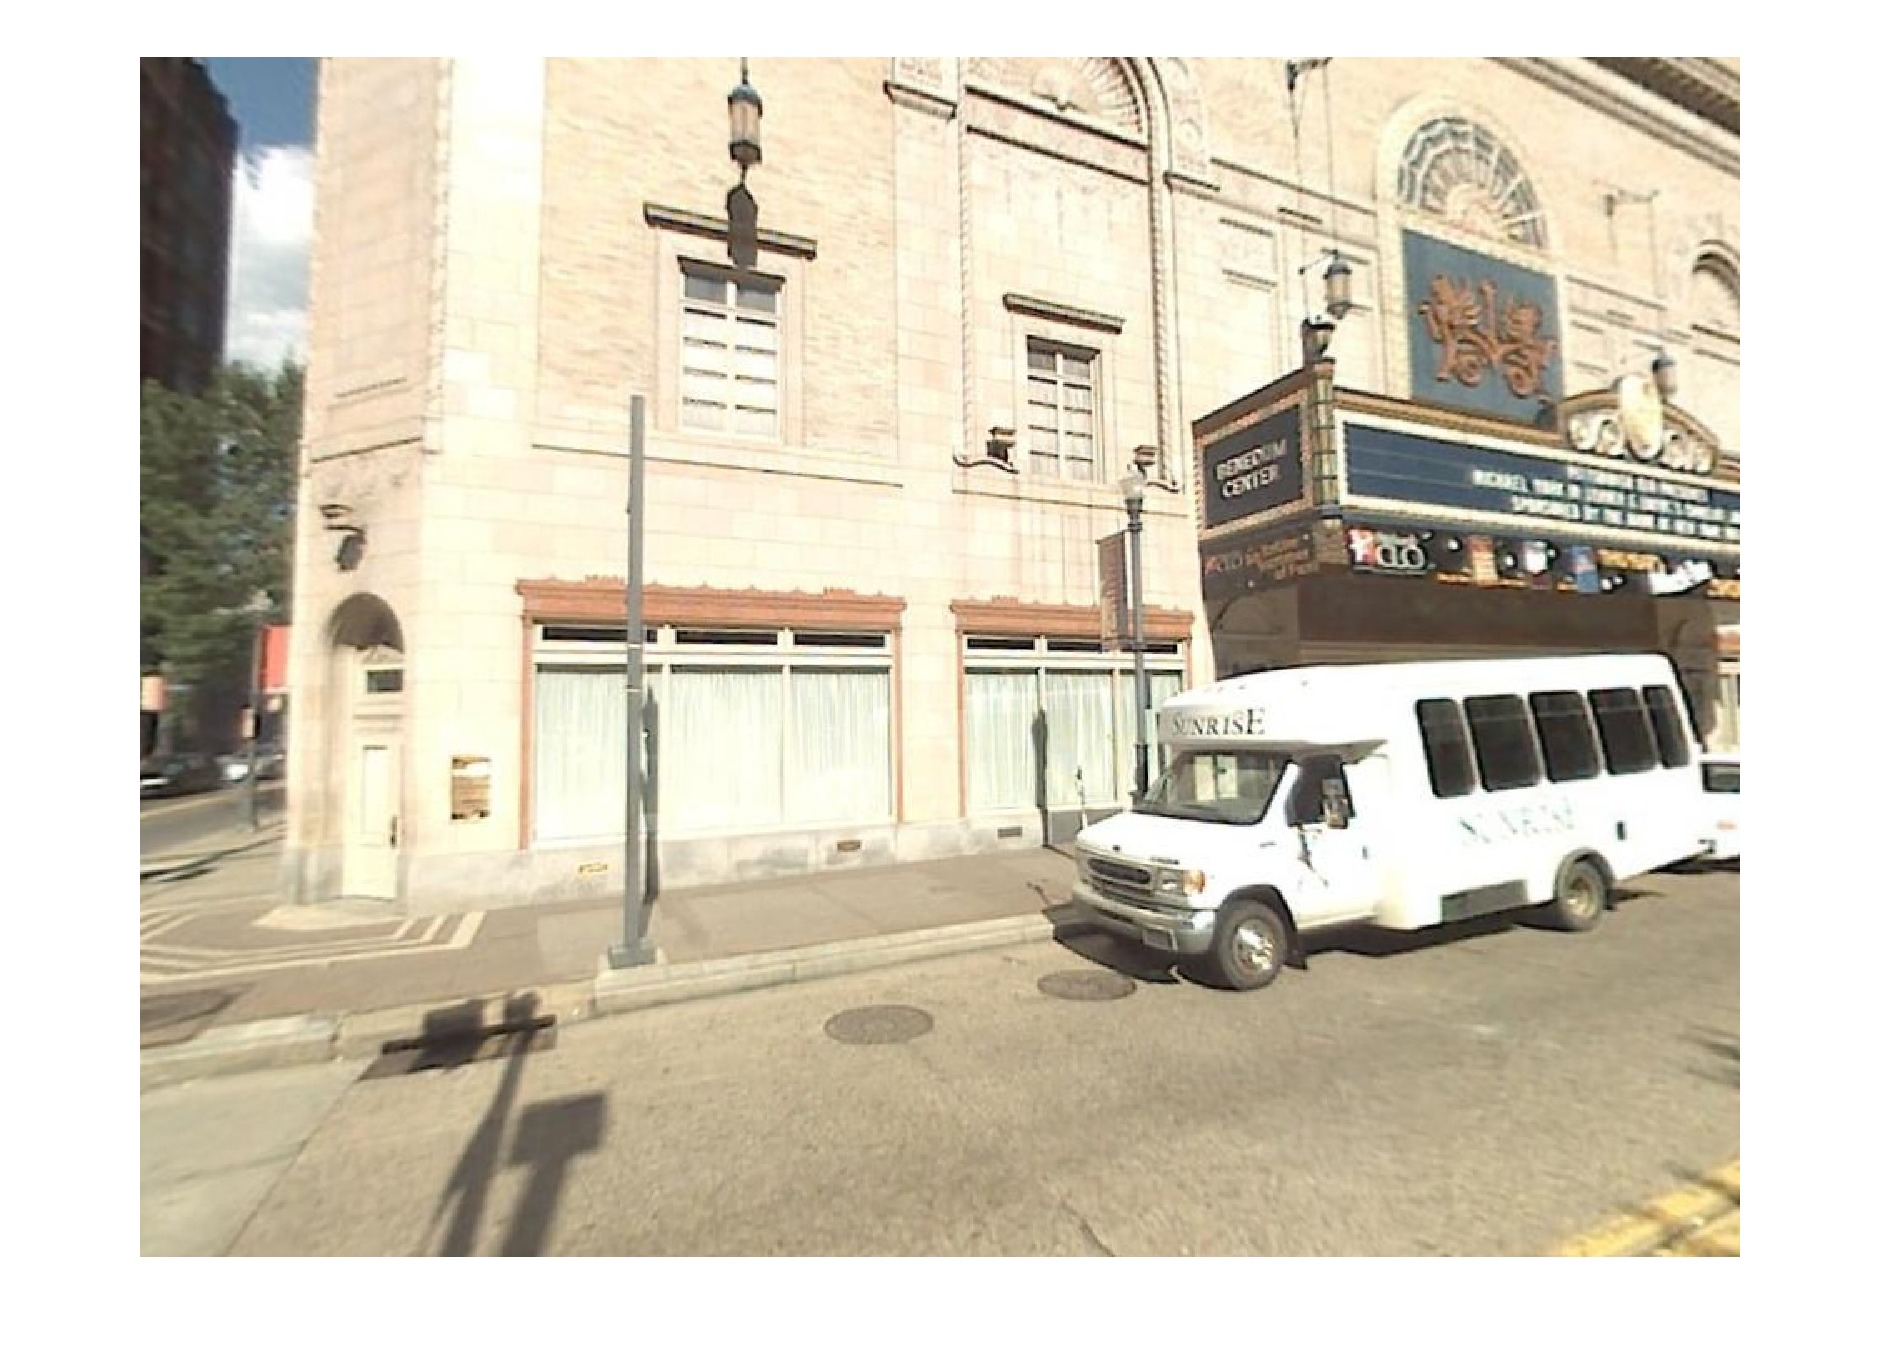
\includegraphics[width=1.05\linewidth]{imgs/aggrv/08aggrvQ.pdf}
		  }
		\end{minipage}
	 }
	 \hspace{3mm}
	 %%%%%%%%%
	 %
	 \colorbox{myRed}{
		\begin{minipage}{\subw}
		  \centerline{
		  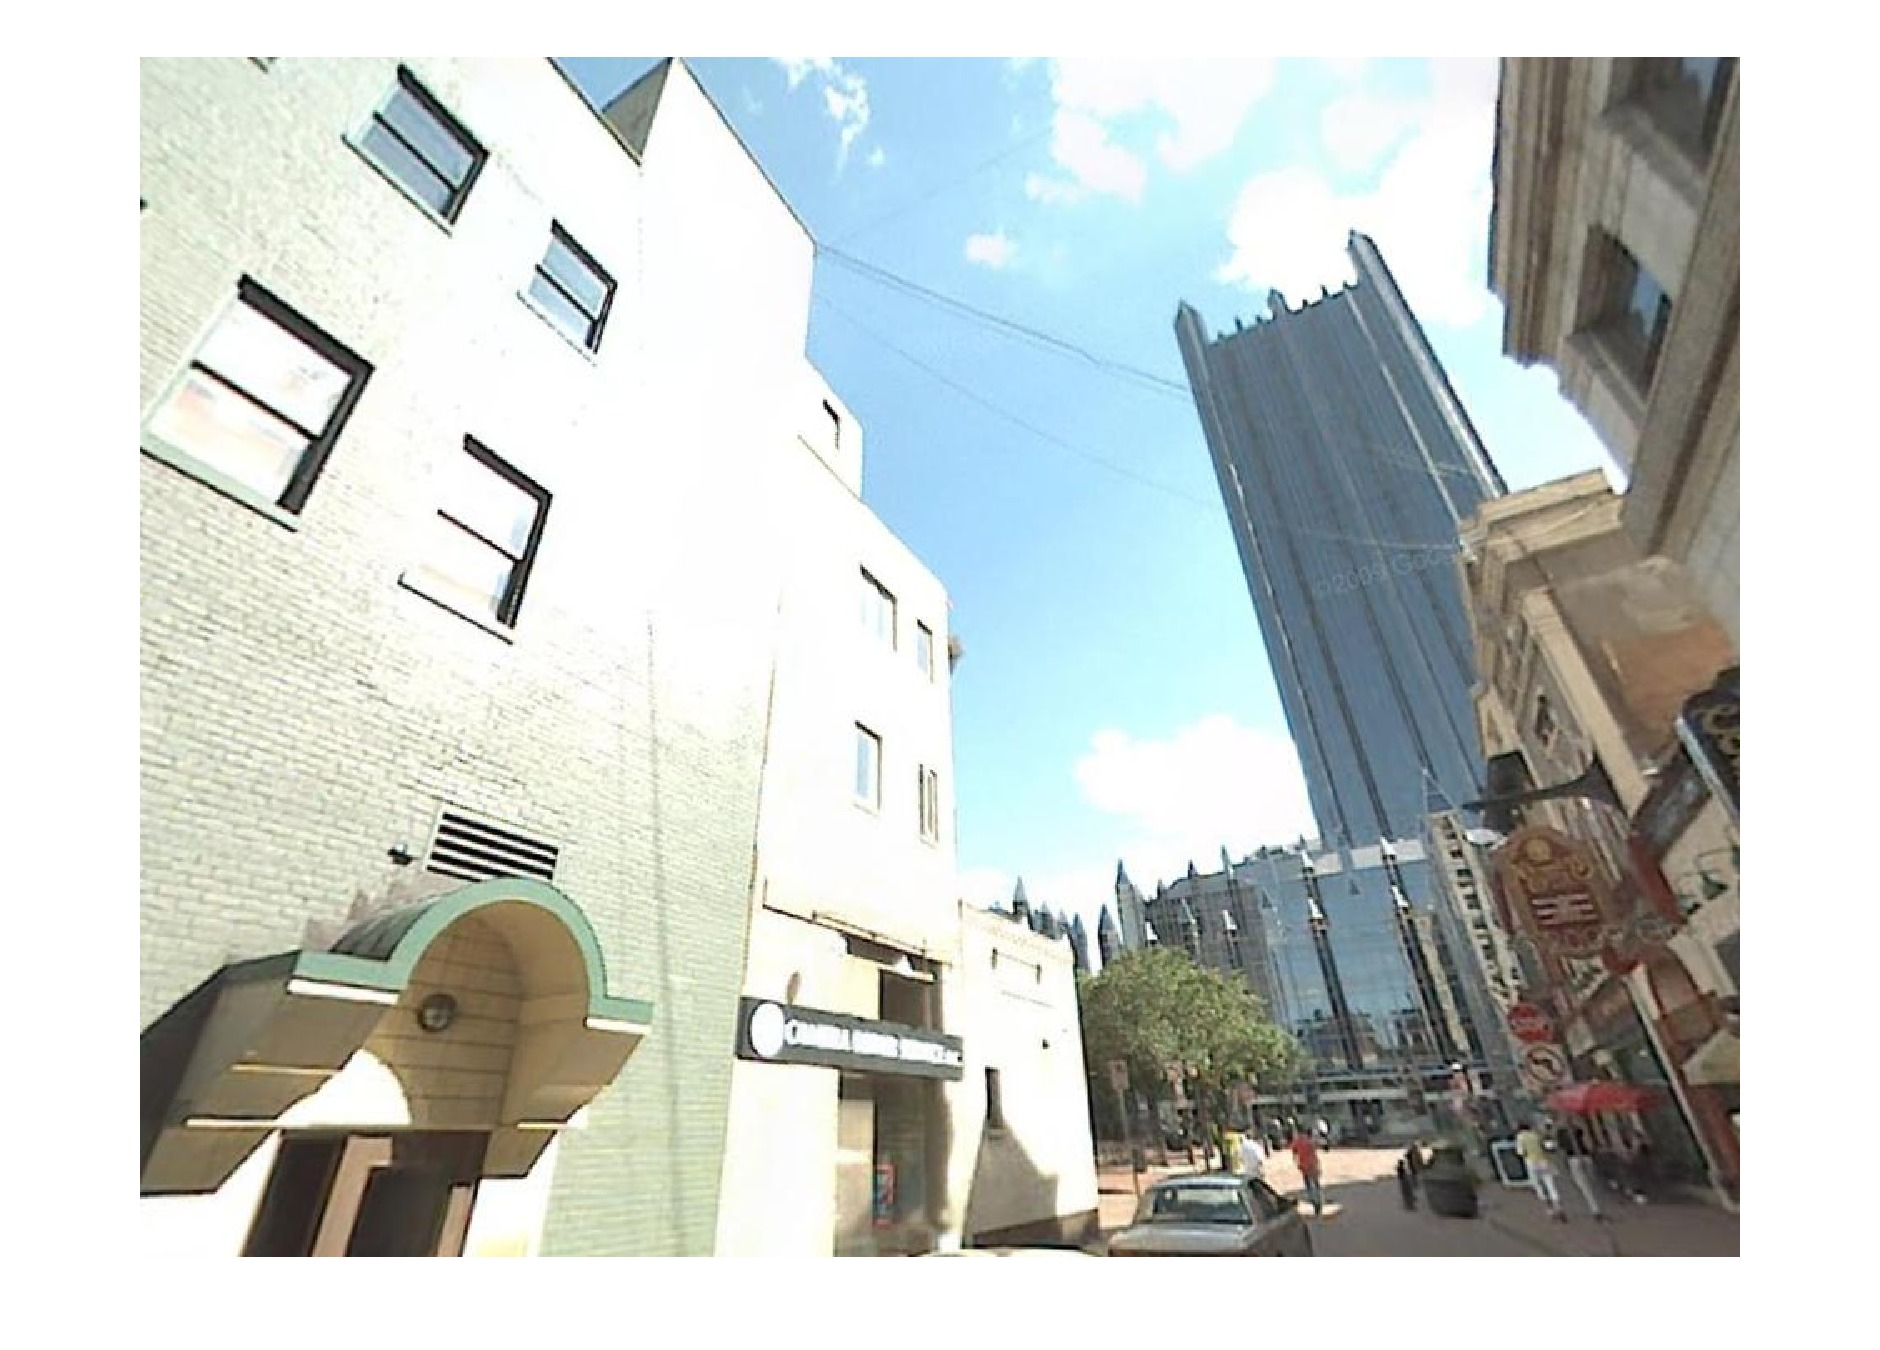
\includegraphics[width=1.05\linewidth]{imgs/aggrv/08aggrvS.pdf}
		  }
		\end{minipage}
	 }
	 %
	 \colorbox{myGreen}{
		\begin{minipage}{\subw}
		  \centerline{
		  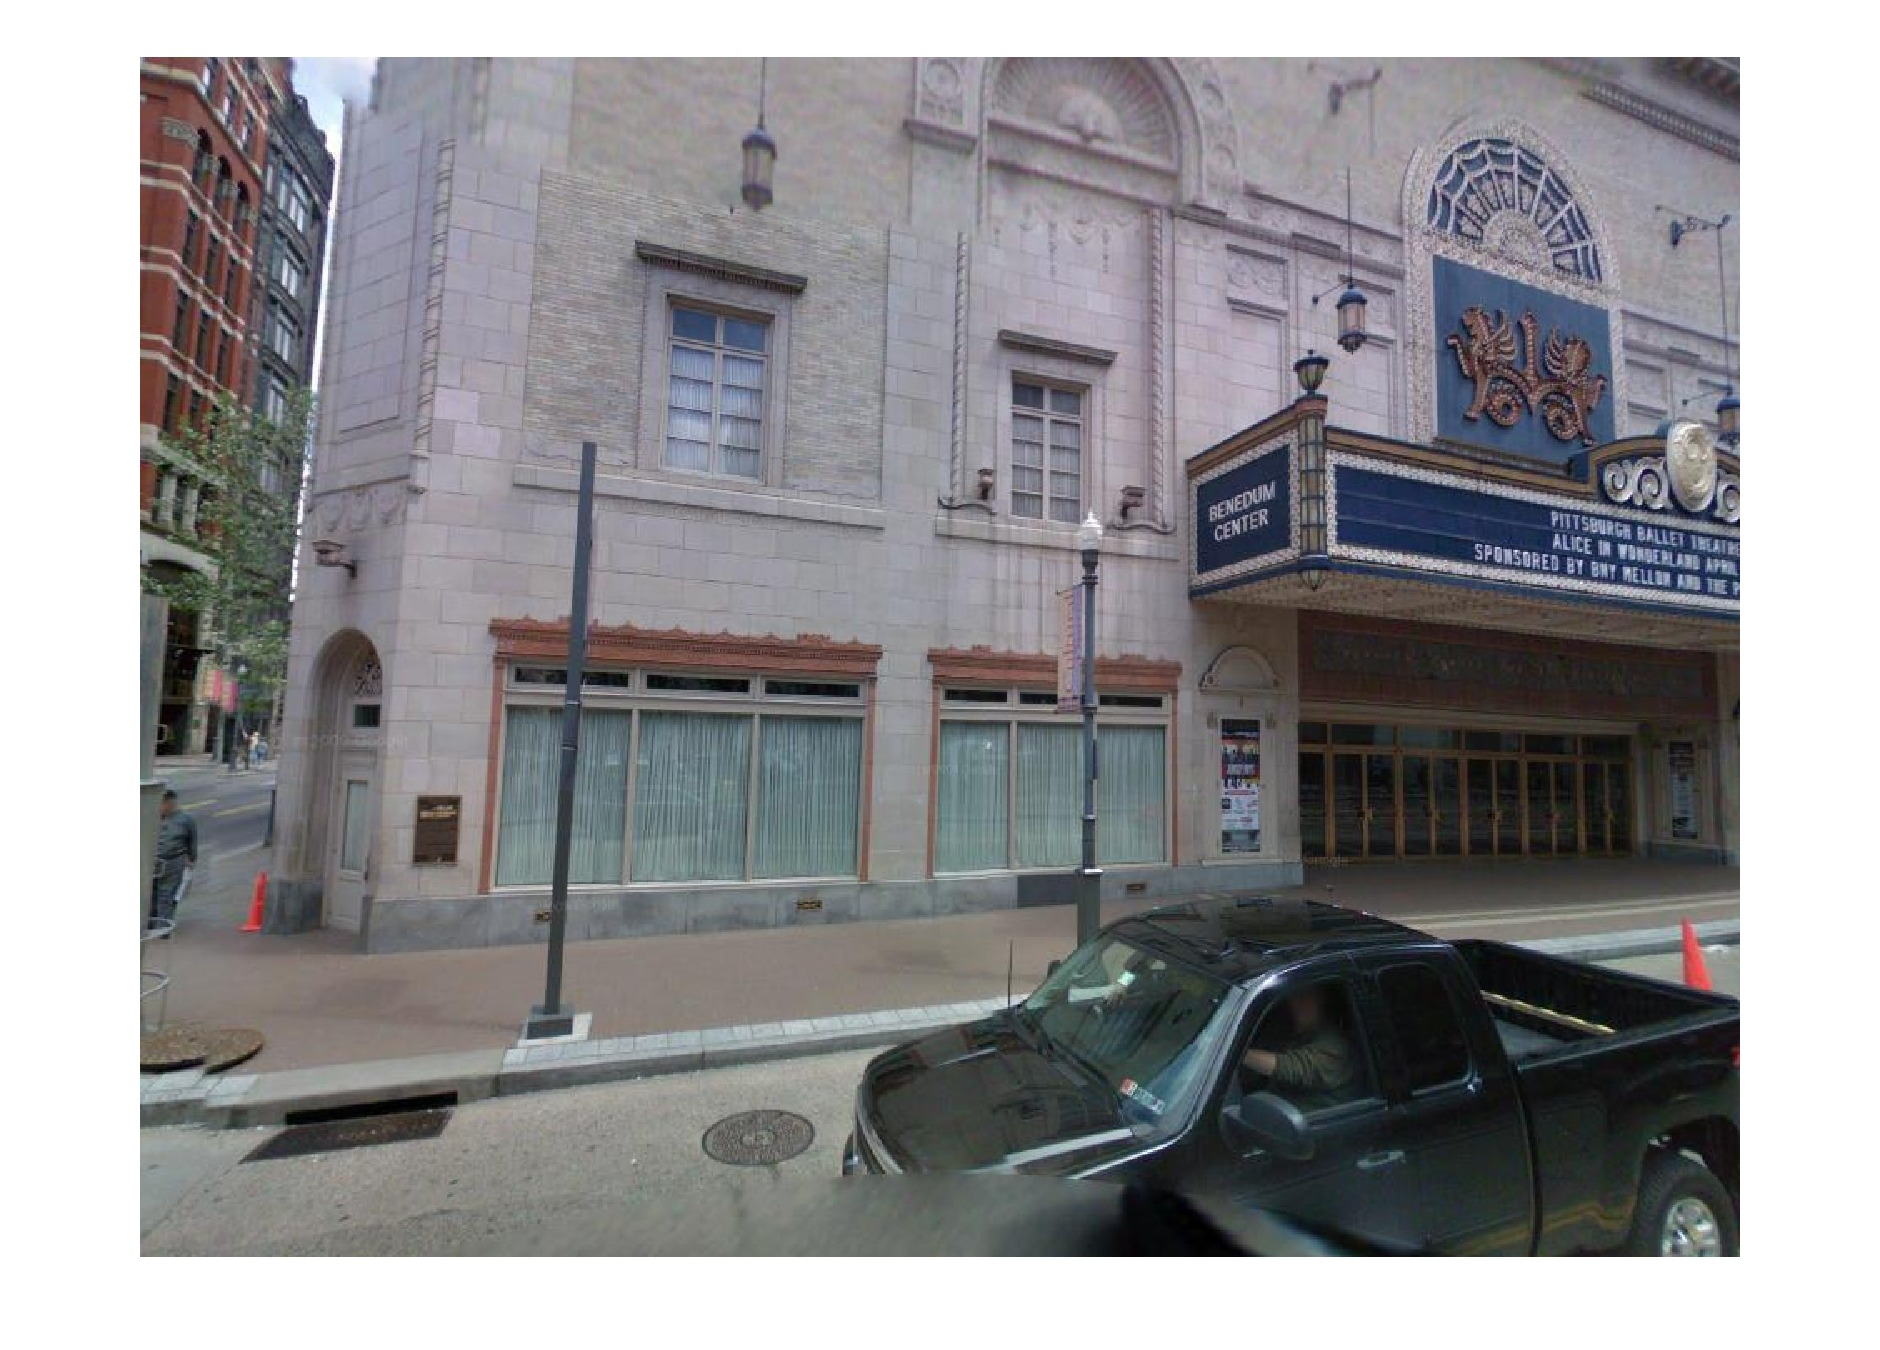
\includegraphics[width=1.05\linewidth]{imgs/aggrv/08aggrvK.pdf}
		  }
		\end{minipage}
	 }
	 %
	 \colorbox{myGreen}{
		\begin{minipage}{\subw}
		  \centerline{
		  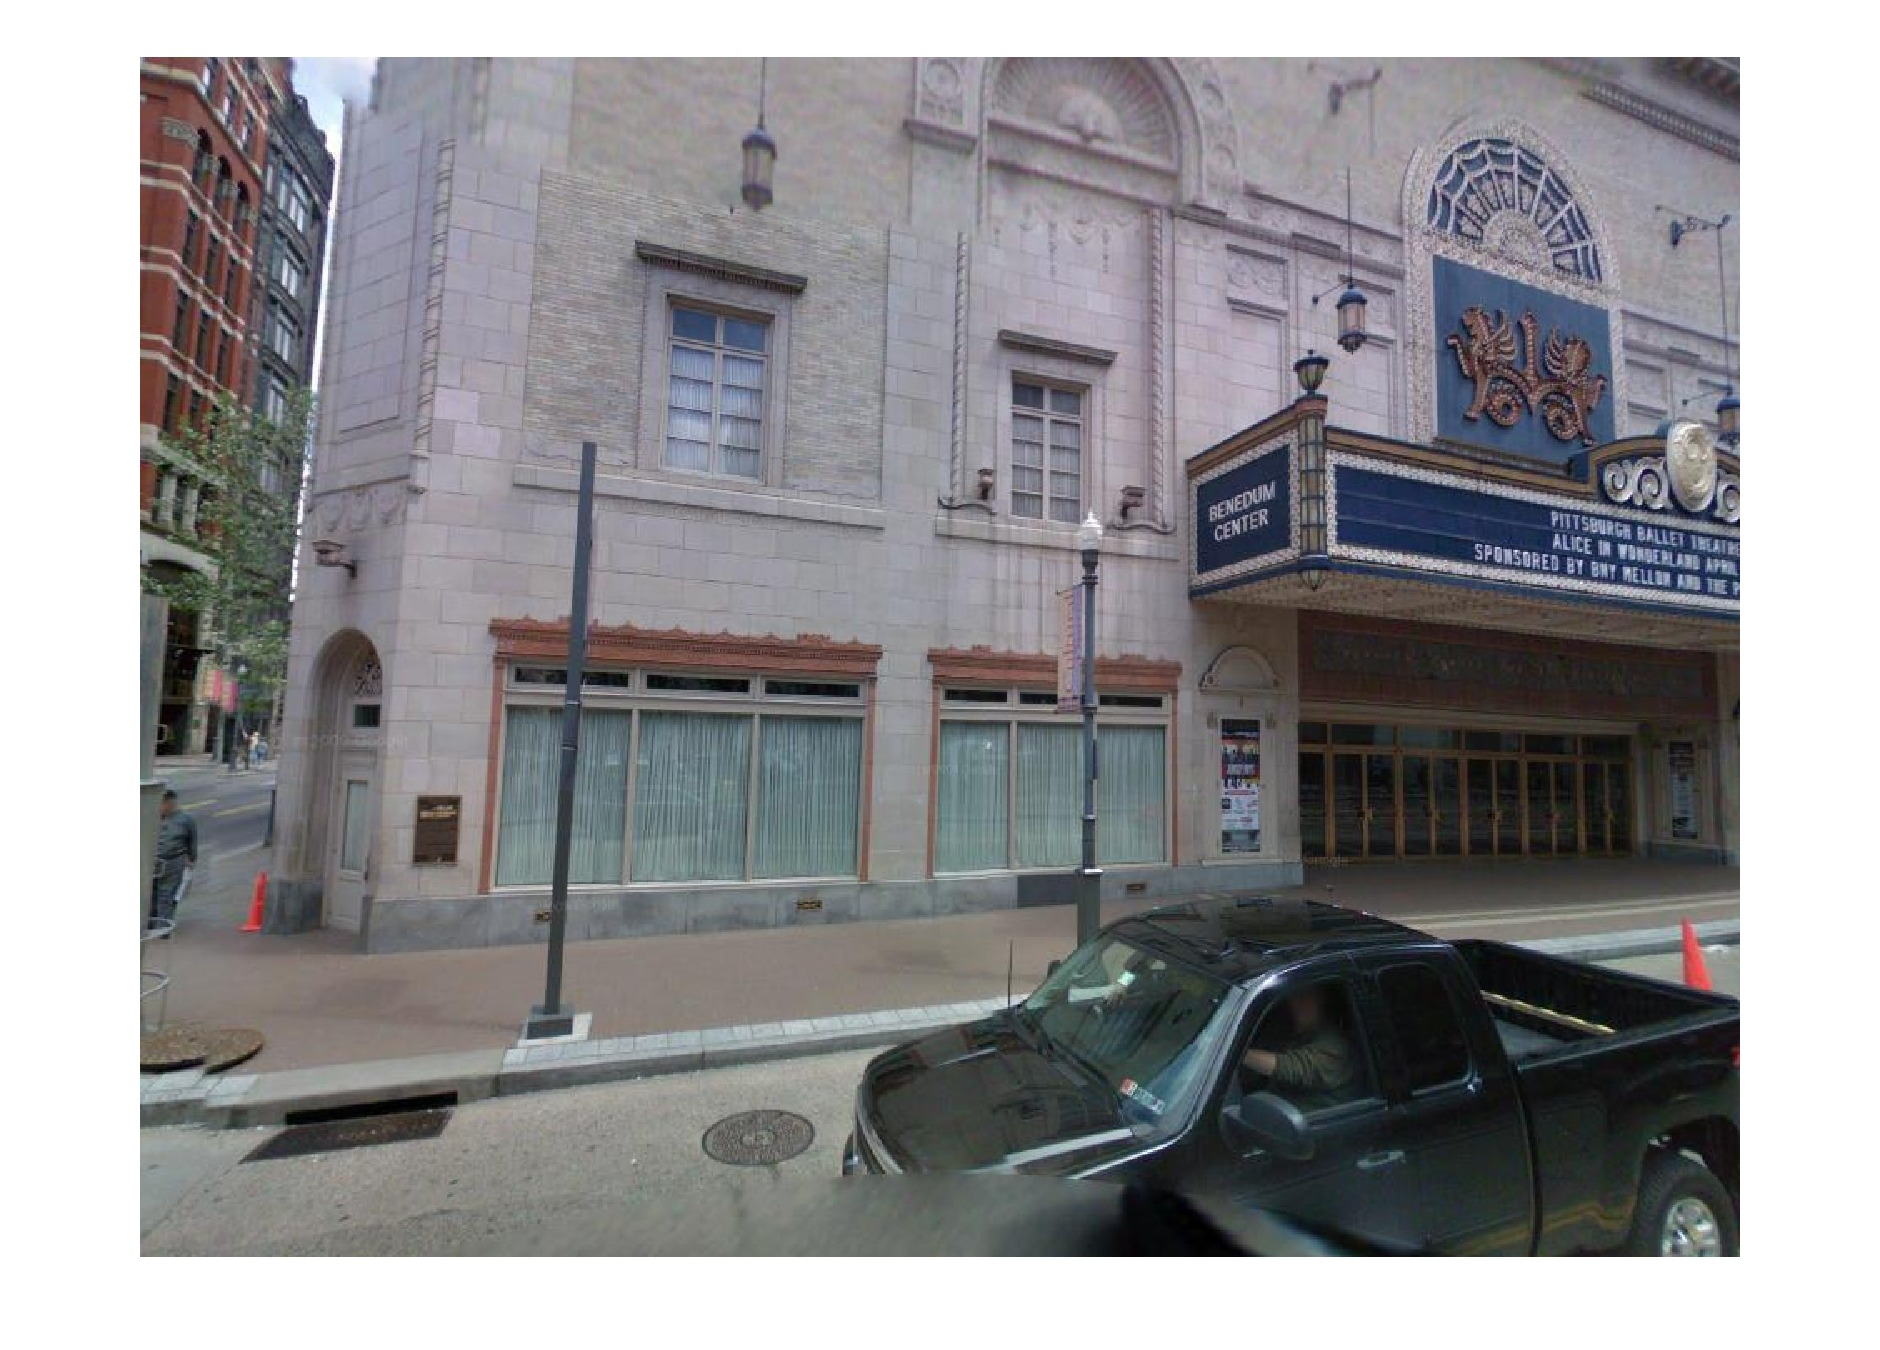
\includegraphics[width=1.05\linewidth]{imgs/aggrv/08aggrvB.pdf}
		  }
		\end{minipage}
	 }
	 \\
	 \begin{minipage}{0.23\linewidth}
		\centering
		(a)
	 \end{minipage}
	 \hspace{3mm}
	 \begin{minipage}{0.23\linewidth}
		\centering
		(b)
	 \end{minipage}
	 \begin{minipage}{0.23\linewidth}
		\centering
		(c)
	 \end{minipage}
	 \begin{minipage}{0.23\linewidth}
		\centering
		(d)
	 \end{minipage}
	 %
	 %
	 \caption{
		{\bf Examples of query images (gray) correctly (green) and incorrectly (red) localized by different methods.} \;(a) query image. \;(b) the top-ranked image retrieved by per-location classifiers (proposed method). \;(c) the top-ranked image retrieved by the baseline confuser suppression method~\cite{Knopp2010}. \;(d) the top-ranked image retrieved by the baseline bag-of-visual-words method.  Bottom two rows: the proposed method is sometimes confused by high-scoring similar repeated texture patterns on facades.
  	}
	\label{fig:demo1}
 \end{figure*}
%%%%%%%%%%%%%%%%%%%%%
\section{Conclusions}
%%%%%%%%%%%%%%%%%%%%%
   We have shown that place recognition can be cast as a classification problem and have used geotags as a readily-available supervision to train an ensemble of classifiers, one for each location in the database. As only few positive examples are available for each location, we have proposed a non-parametric procedure to calibrate the output of each classifier without the need for additional positive training data. The results show improved place recognition performance over baseline methods and demonstrate that careful calibration is critical to achieve competitive place recognition performance. The developed calibration method is not specific to place recognition and can be useful for other per-exemplar classification tasks, where only a small number of positive examples are available~\cite{Malisiewicz11}.

   \vspace*{-3mm}


\begin{acknowledgements}
   This work was supported by the MSR-INRIA laboratory, the EIT-ICT labs, PRoViDE EU FP7-SPACE-312377 project and SGS13/140/OHK3/2T/13.
   {
   \footnotesize
   \noindent
   Supported by the Intelligence Advanced Research Projects Activity (IARPA) via Air Force Research Laboratory. The U.S. Government is authorized to reproduce and distribute reprints for governmental purposes notwithstanding any copyright annotation thereon. Disclaimer:  The views and conclusions contained herein are those of the authors and should not be interpreted as necessarily representing the official policies or endorsements, either expressed or implied, of IARPA, AFRL or the U.S. Government.
   }
\end{acknowledgements}

  \begin{figure*}%[tbp]
  \begin{minipage}{0.48\linewidth}
          \begin{minipage}{0.65\linewidth}
            \centering
            {\scriptsize Calibrated classifier score $f_j$}
            \\
            \vspace{2mm}
            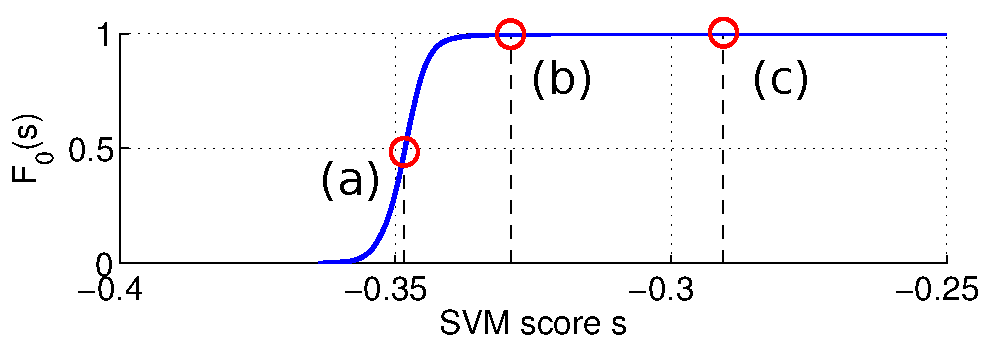
\includegraphics[width=\linewidth]{imgs/wVS3q/2882/graphBigO.pdf}
          \end{minipage} 
          %
          \begin{minipage}{\wii}
            \centering
            \centerline{\scriptsize Target database image $j$}
            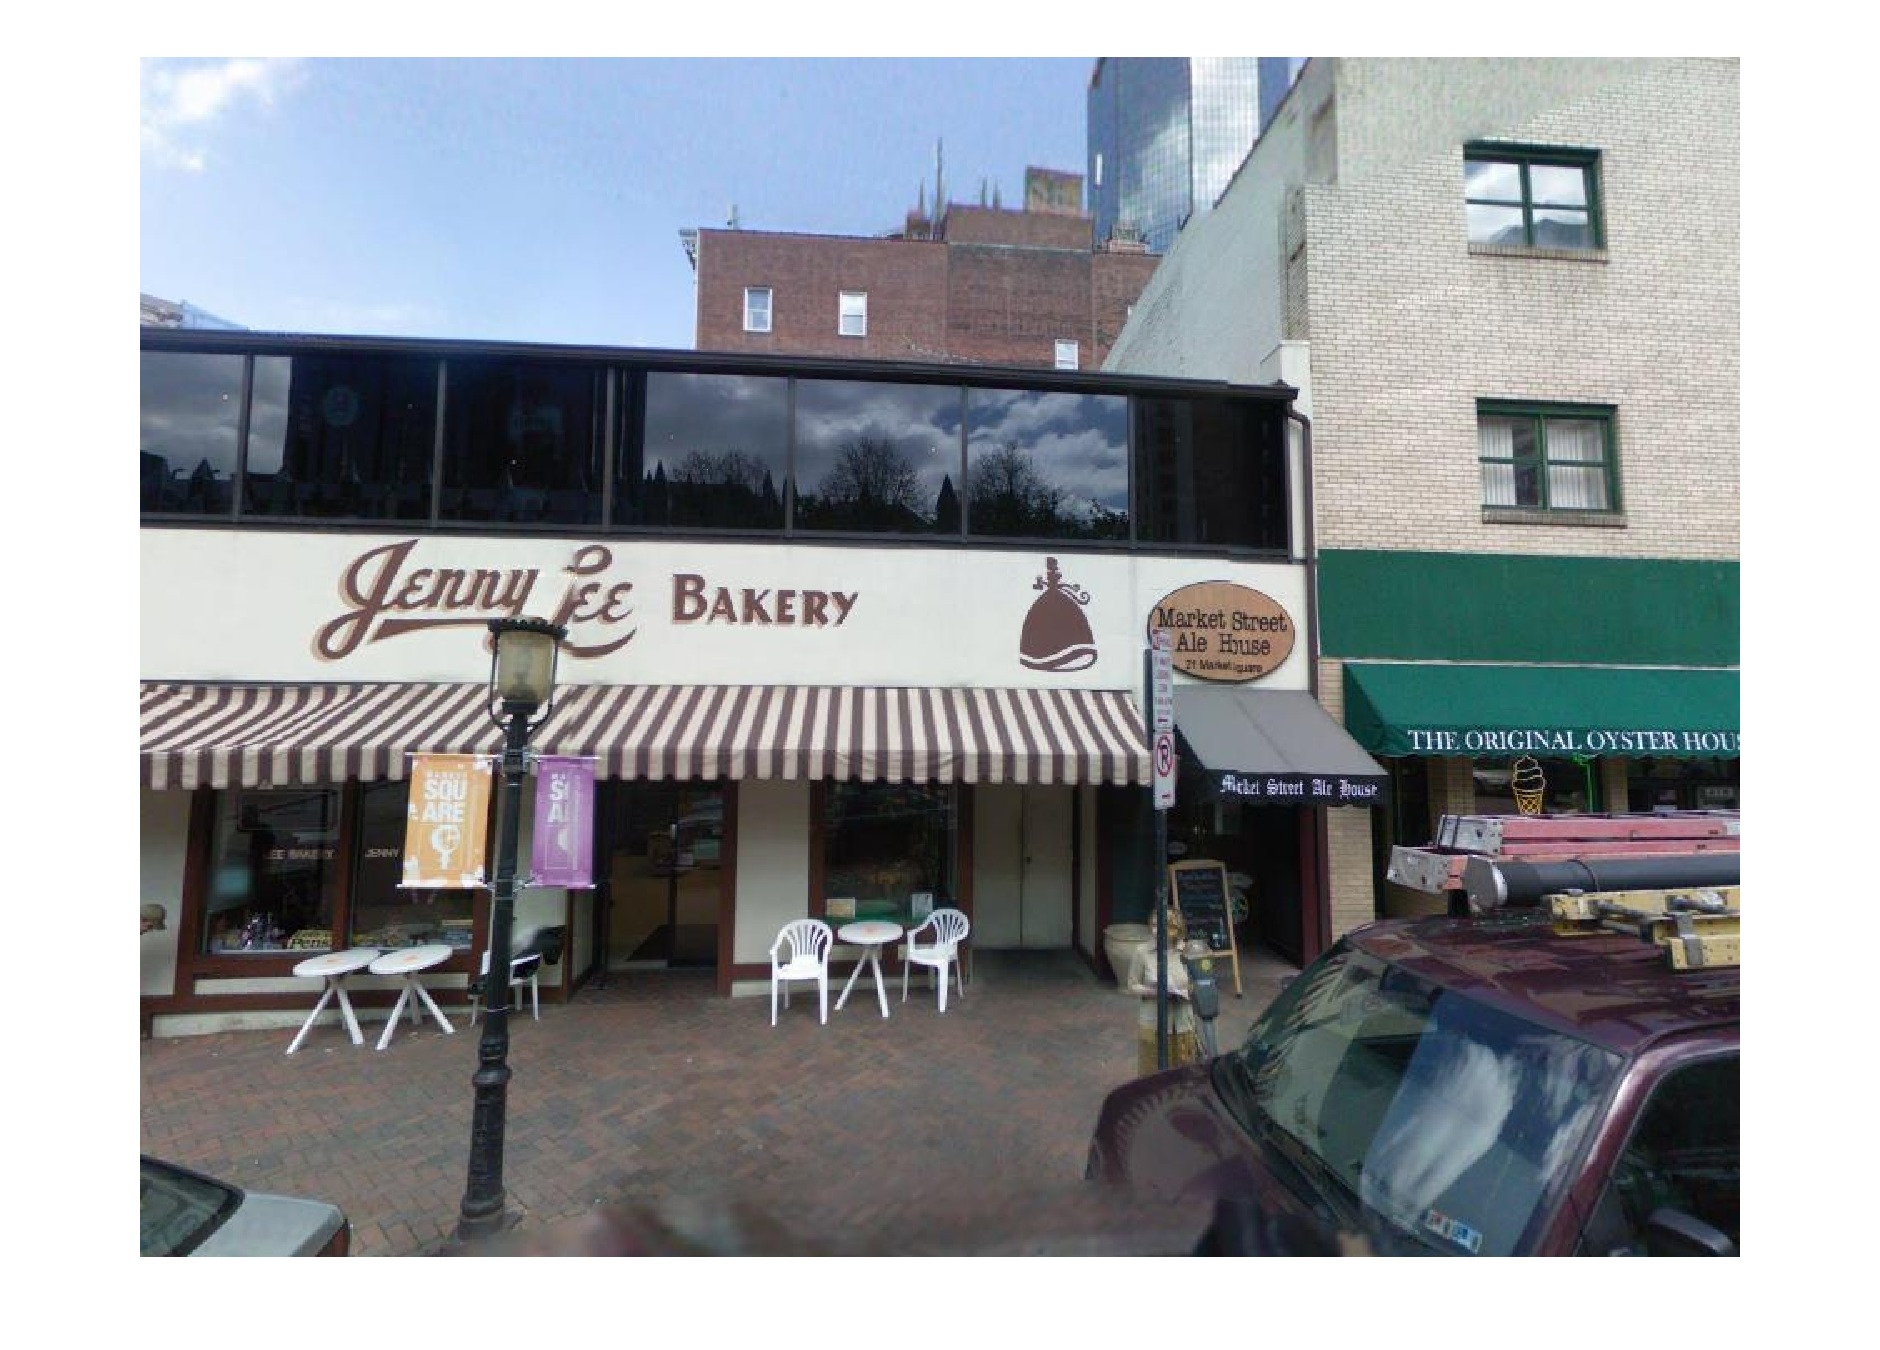
\includegraphics[width=\linewidth]{imgs/wVS3q/2882/j.jpg}
          \end{minipage}  
          \vspace{3mm}
          \\
          \centerline{\scriptsize Classified query images $f_j(q)$} 
          \\
          \begin{minipage}{\wii}
            \centering
            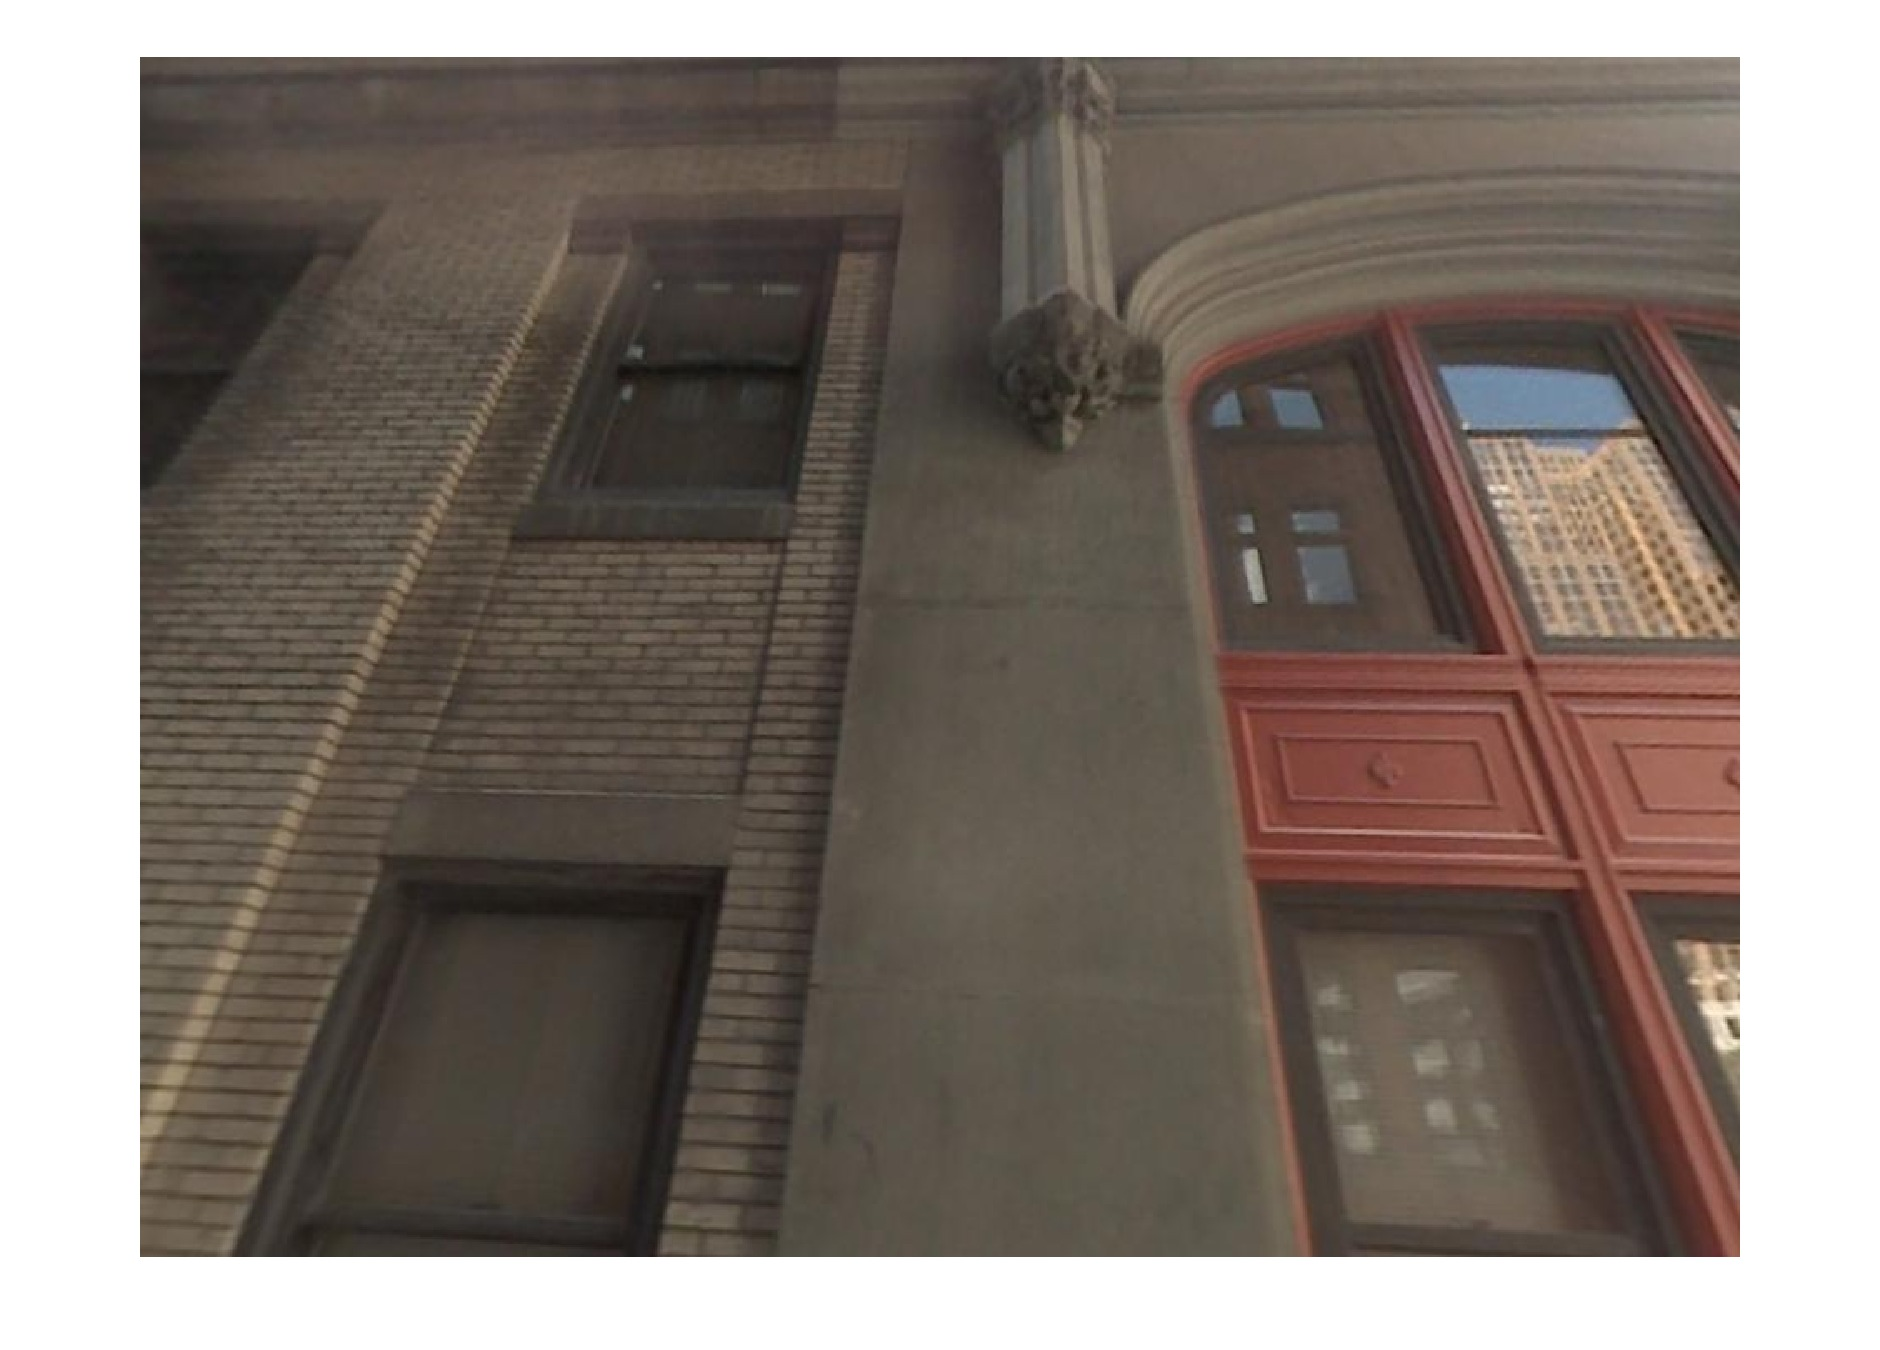
\includegraphics[width=\linewidth]{imgs/wVS3q/2882/a.jpg}
          \end{minipage}
          %  
          \begin{minipage}{\wii}
            \centering
            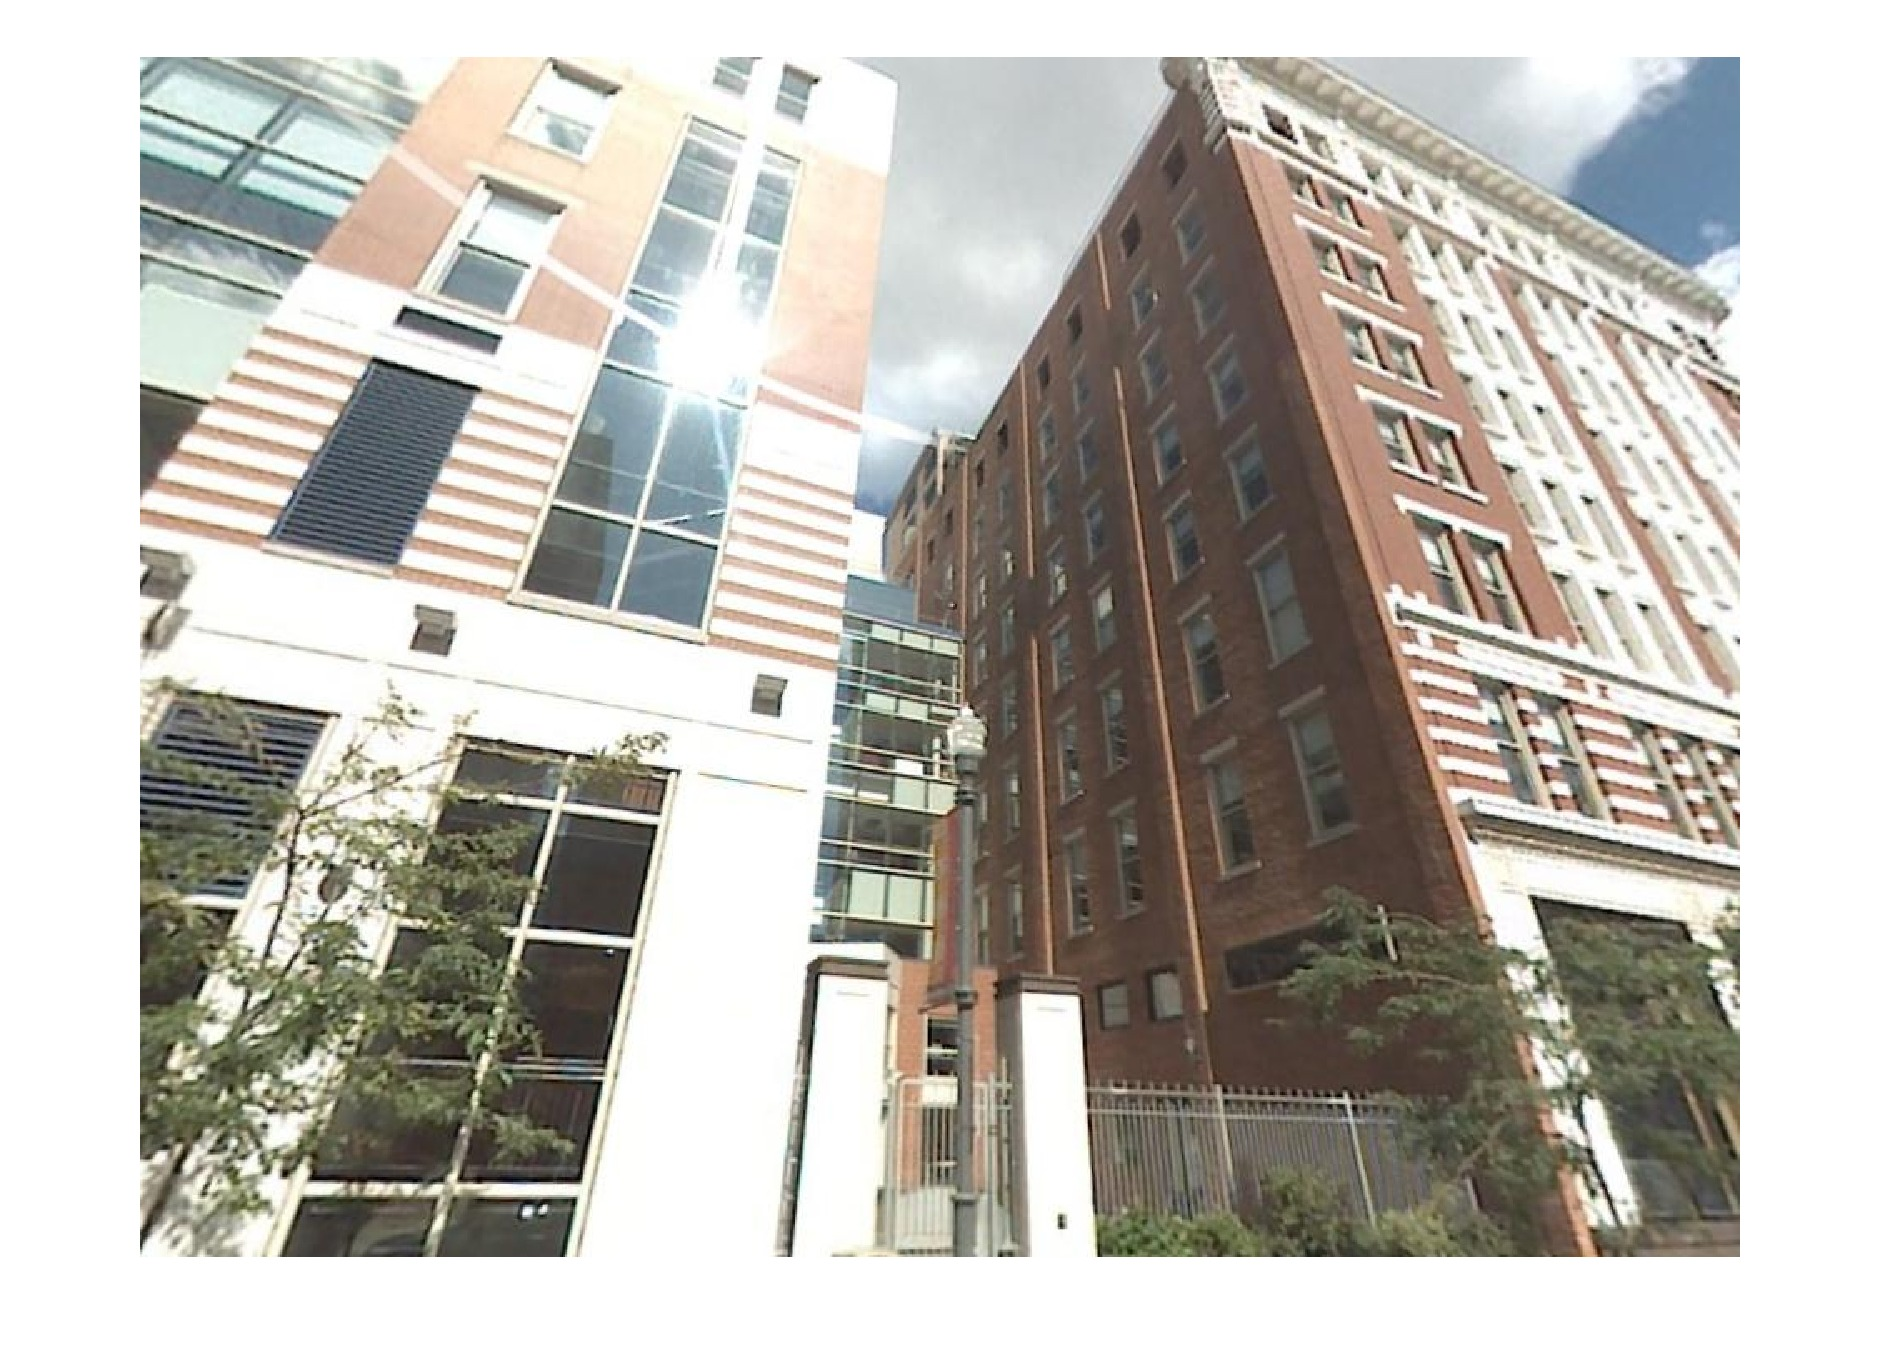
\includegraphics[width=\linewidth]{imgs/wVS3q/2882/b.jpg}
          \end{minipage}
          %  
          \begin{minipage}{\wii}
            \centering
            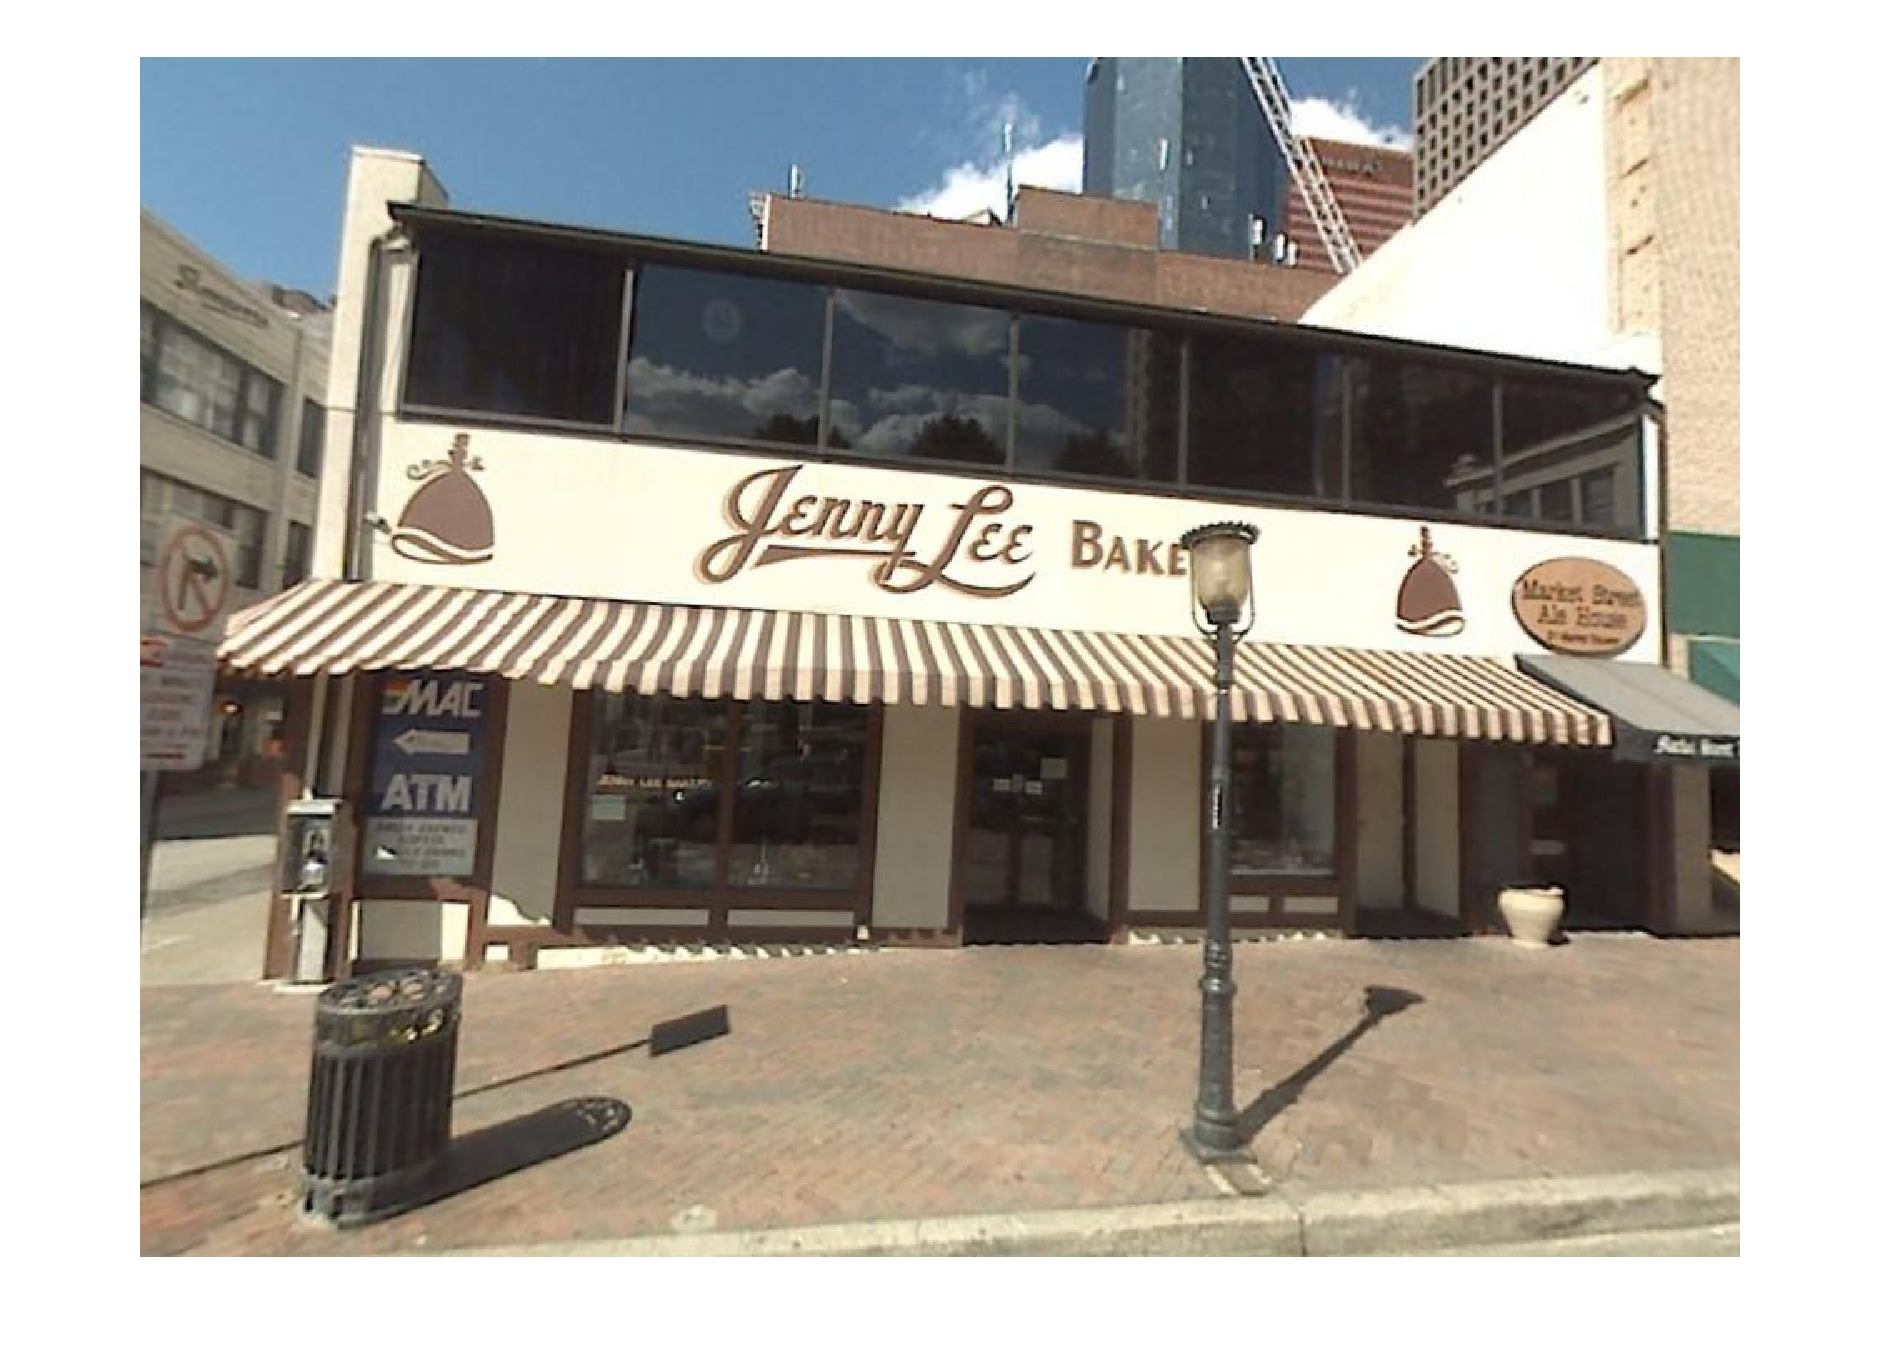
\includegraphics[width=\linewidth]{imgs/wVS3q/2882/c.jpg}
          \end{minipage} 
          \\
          \begin{minipage}{\wii}
            \centering
            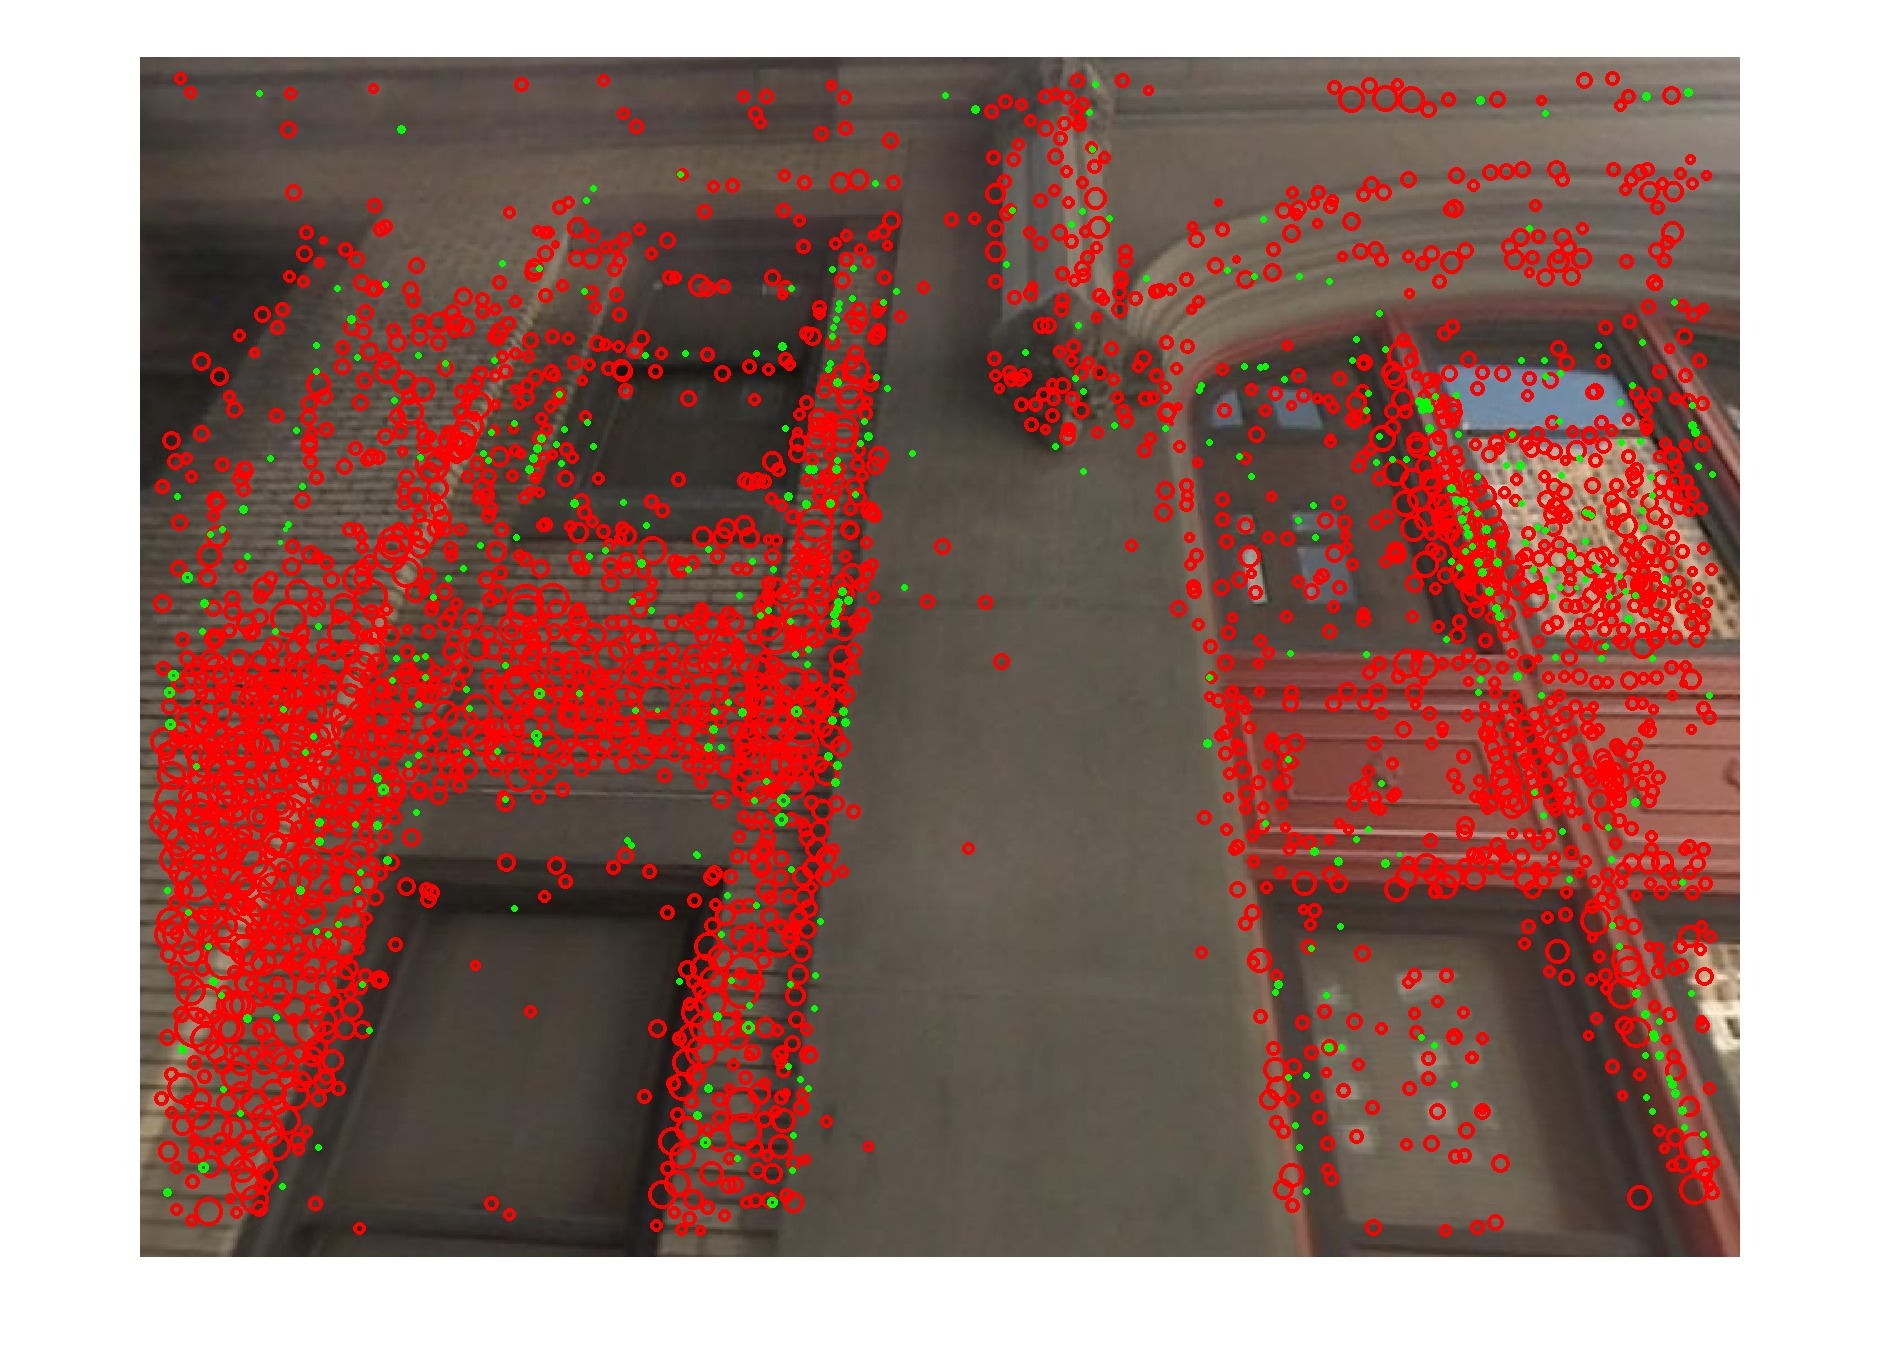
\includegraphics[width=\linewidth]{imgs/wVS3q/2882/aftrs.jpg}
            \newline
            (a)
          \end{minipage}  
          \begin{minipage}{\wii}
            \centering
            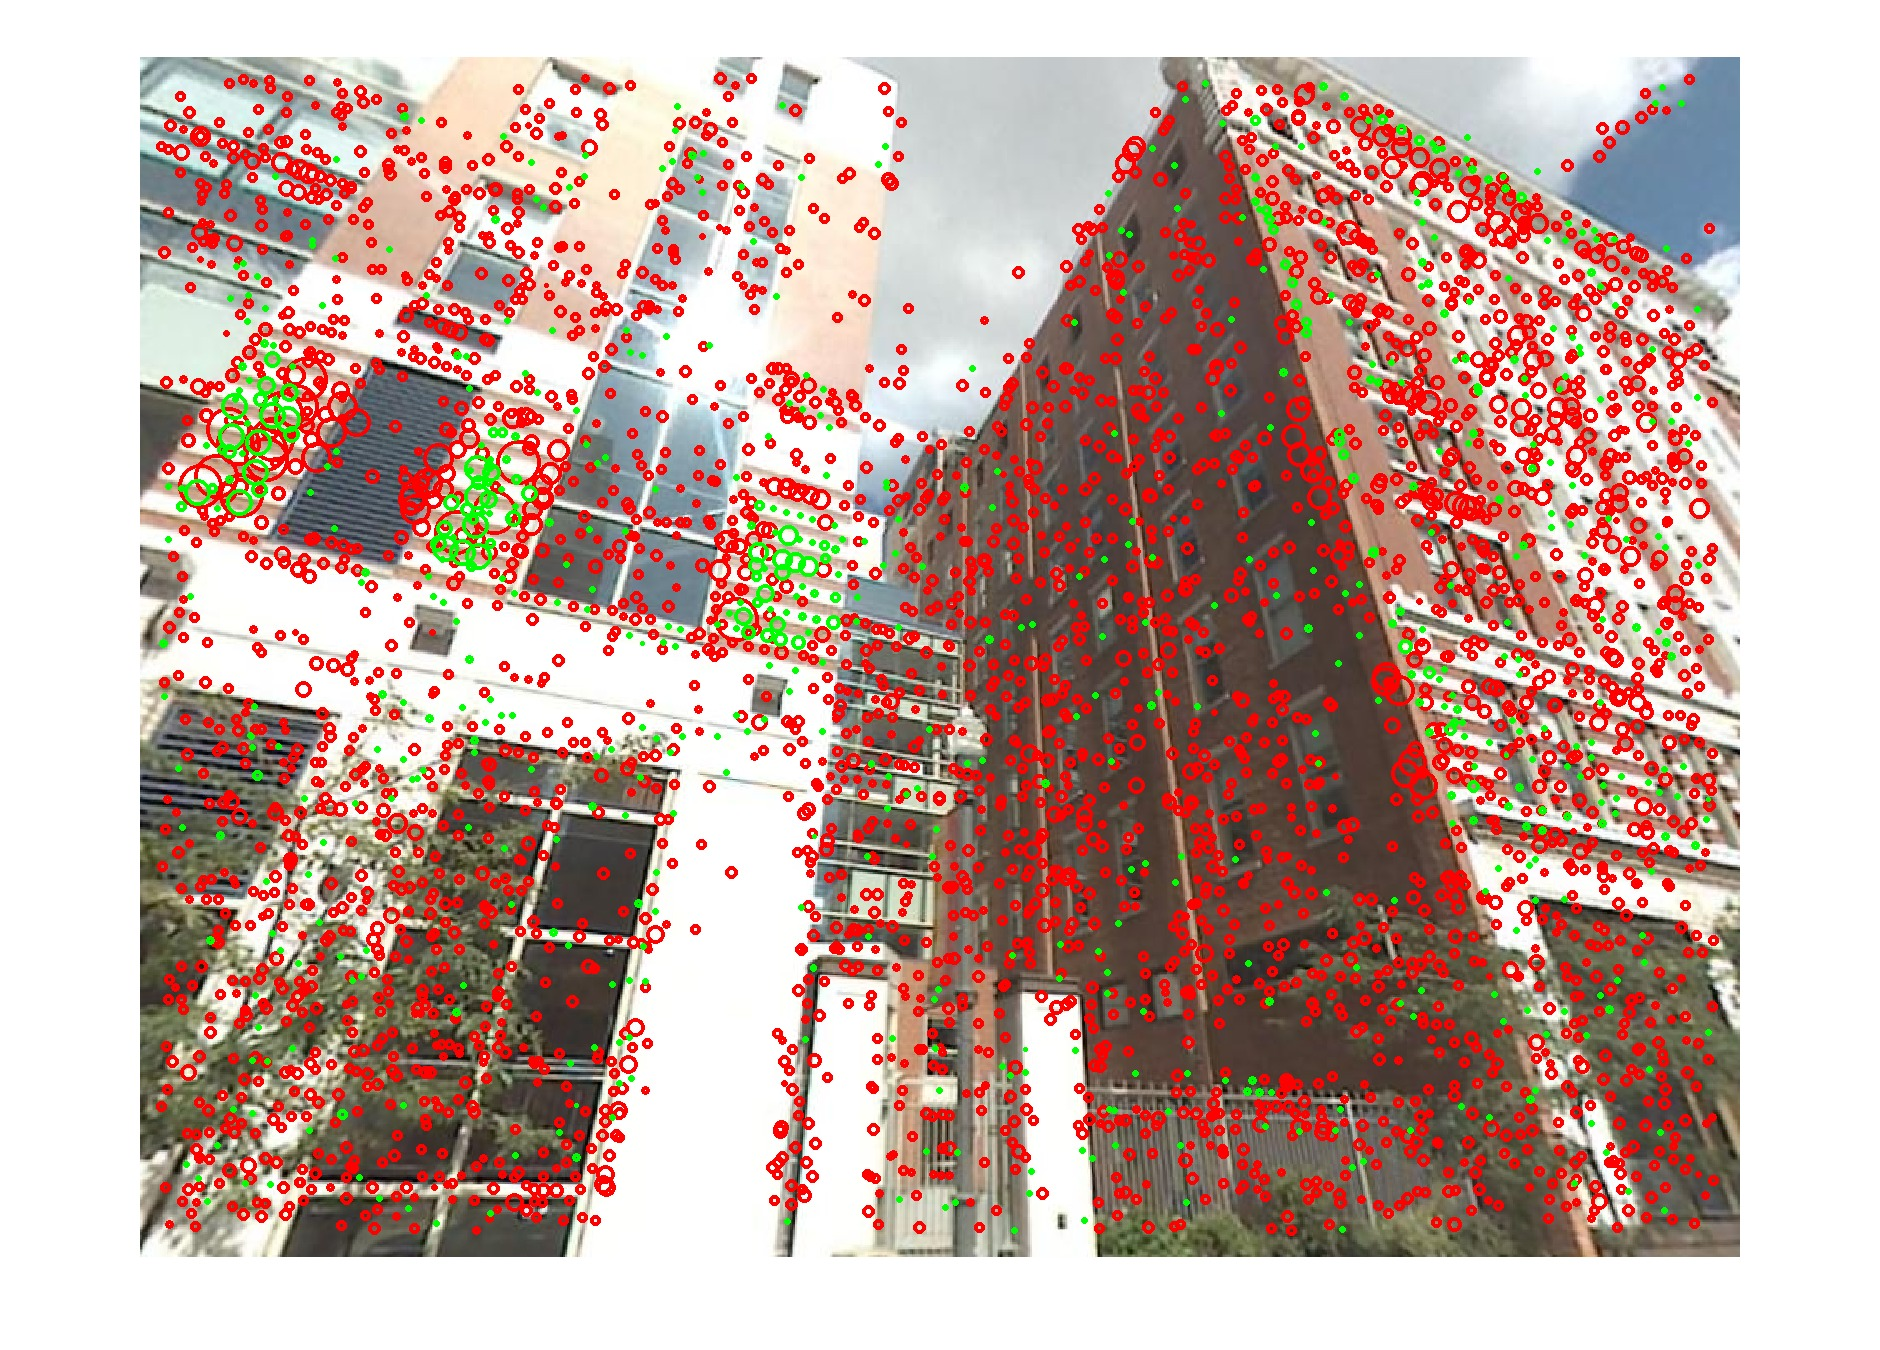
\includegraphics[width=\linewidth]{imgs/wVS3q/2882/bftrs.jpg}
            \newline
            (b)
          \end{minipage}  
          \begin{minipage}{\wii}
            \centering
            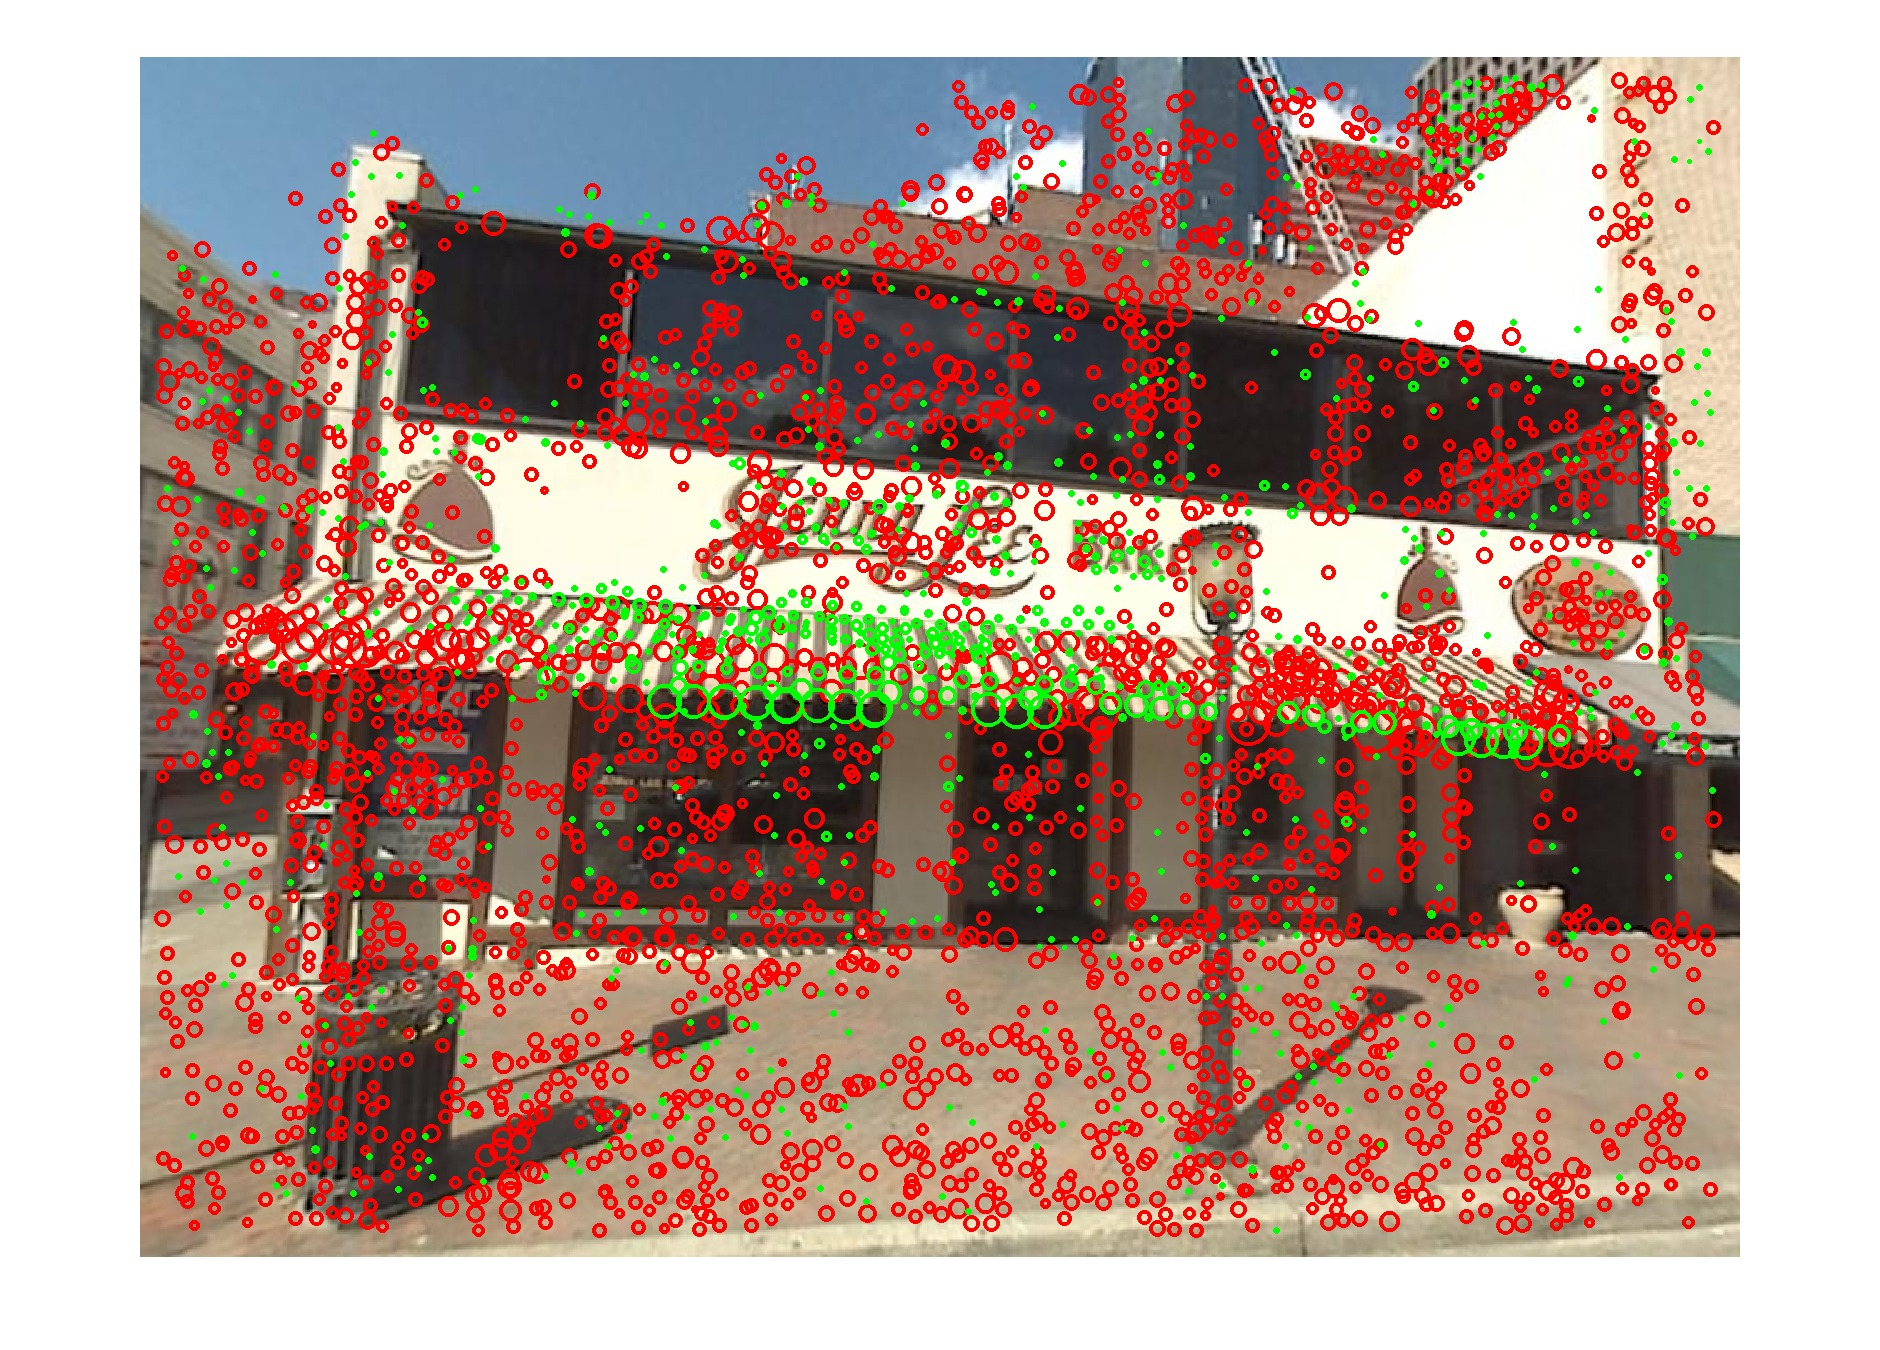
\includegraphics[width=\linewidth]{imgs/wVS3q/2882/cftrs.jpg}
            \newline
            (c)
          \end{minipage} 
    \end{minipage}% left figure
    %
    %%%%%%%%%%%%%%%%%%%%%%%%%%%%%%%%%
    \begin{minipage}{0.04\linewidth}
      \hspace{\linewidth}
    \end{minipage}
    %%%%%%%%%%%%%%%%%%%%%%%%%%%%%%%%%
    % RIGHT FIGURE
    \begin{minipage}{0.48\linewidth}
          \begin{minipage}{0.66\linewidth}
            \centering
            {\scriptsize Calibrated classifier score $f_j$}
            \\
            \vspace{2mm}
            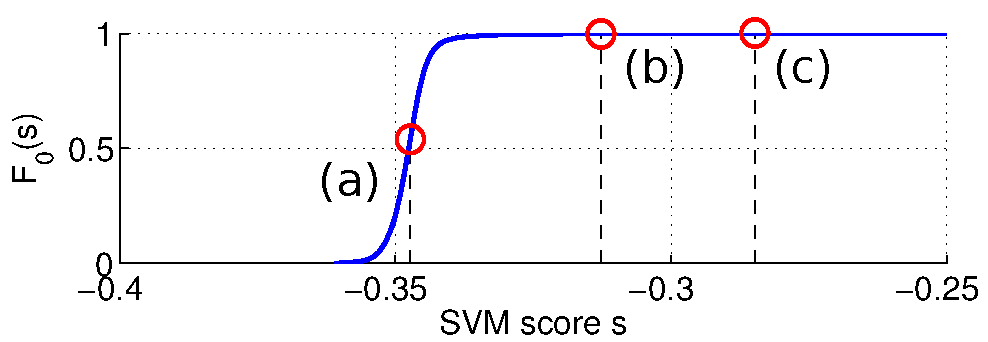
\includegraphics[width=\linewidth]{imgs/wVS3q/2932/graphBigO.pdf}
          \end{minipage} 
          %
          \begin{minipage}{\wii}
            \centering
            \centerline{\scriptsize Target database image $j$}
            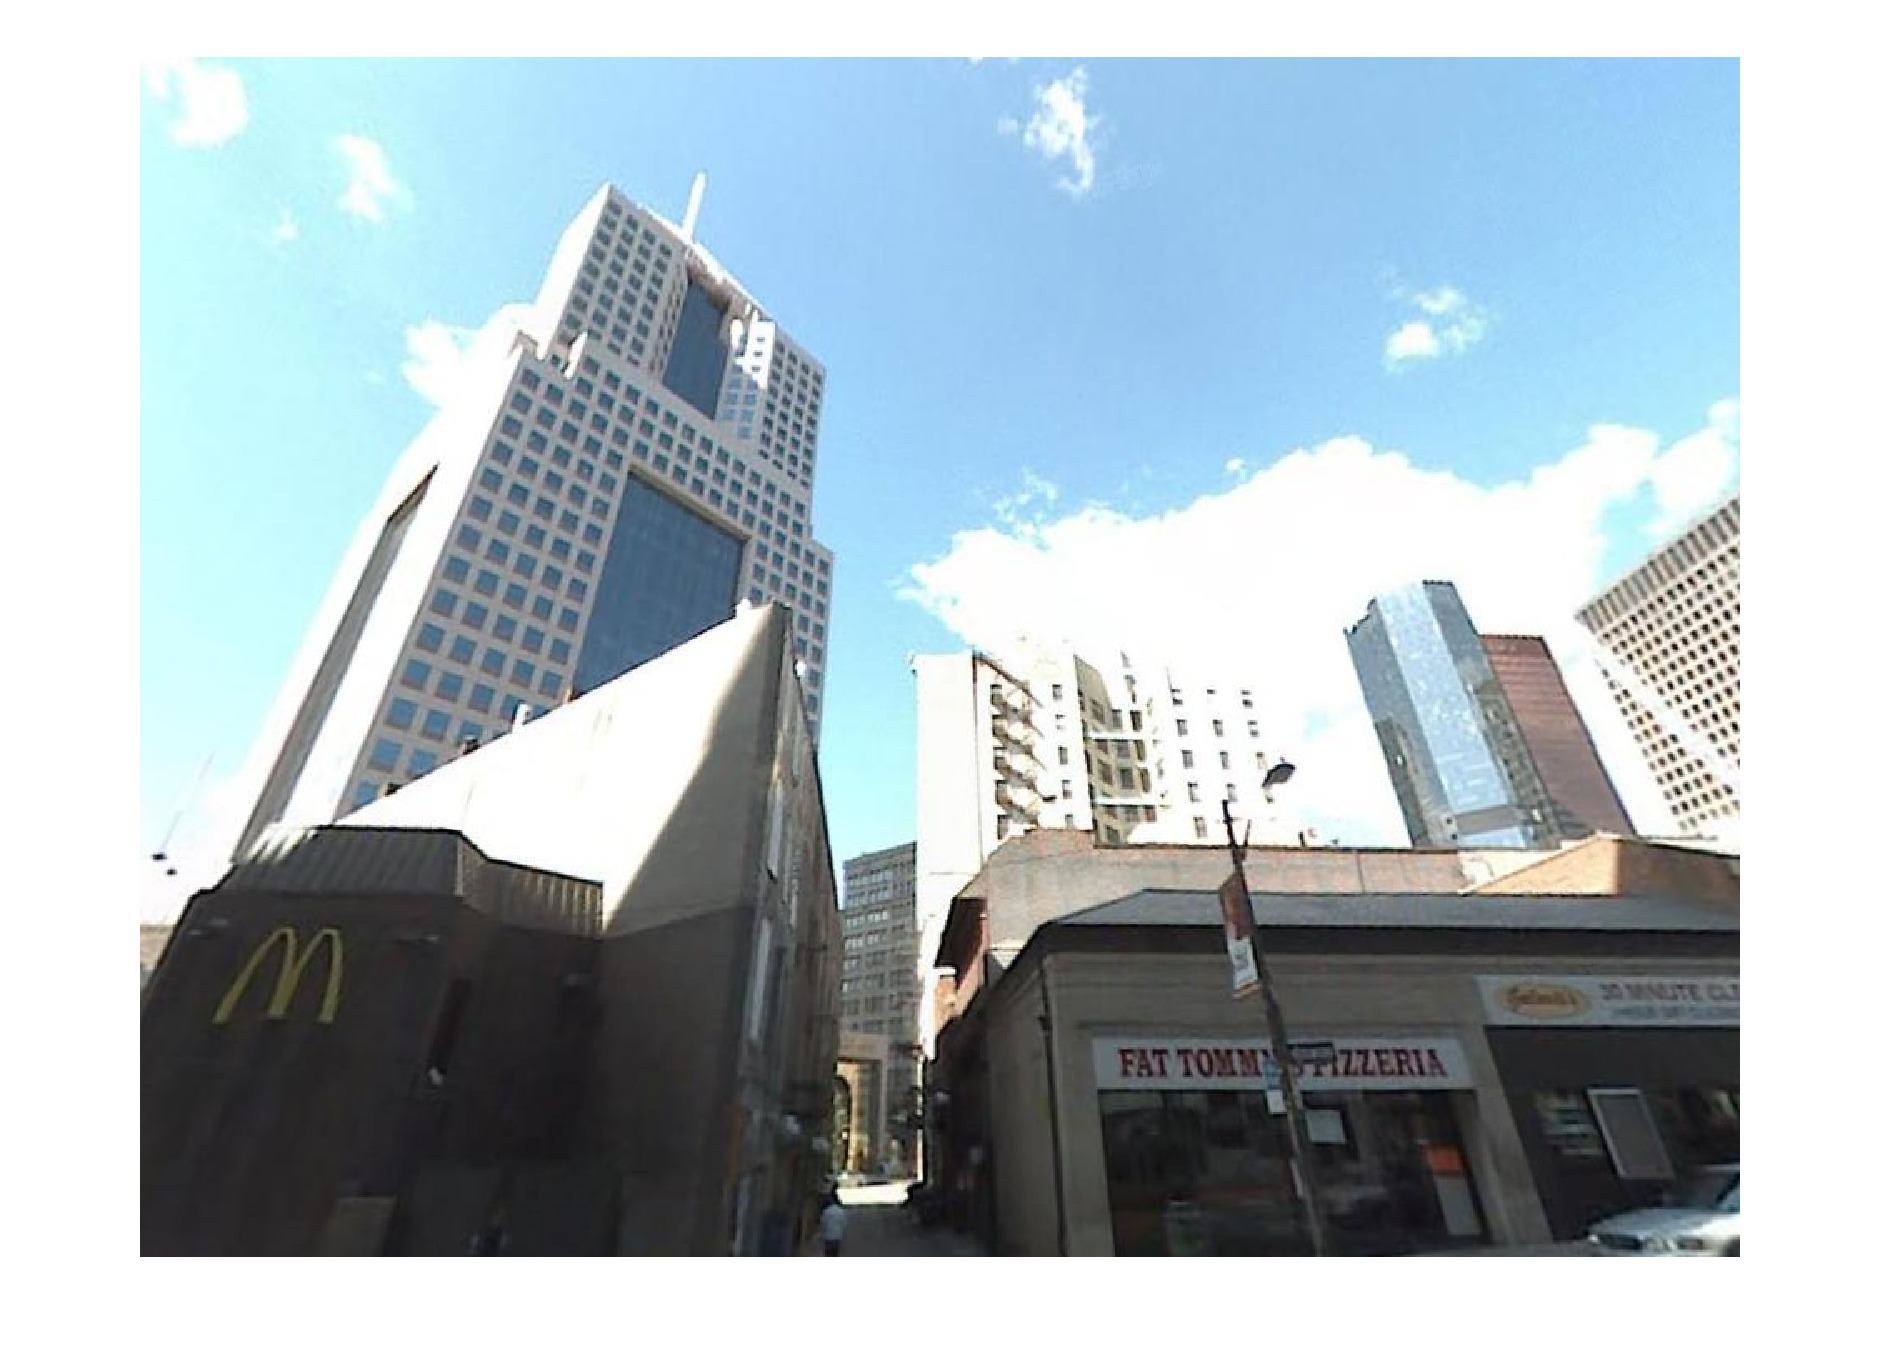
\includegraphics[width=\linewidth]{imgs/wVS3q/2932/j.jpg}
          \end{minipage}  
          \vspace{3mm}
          \\
          \centerline{\scriptsize Classified query images $f_j(q)$} 
          \\
          \begin{minipage}{\wii}
            \centering
            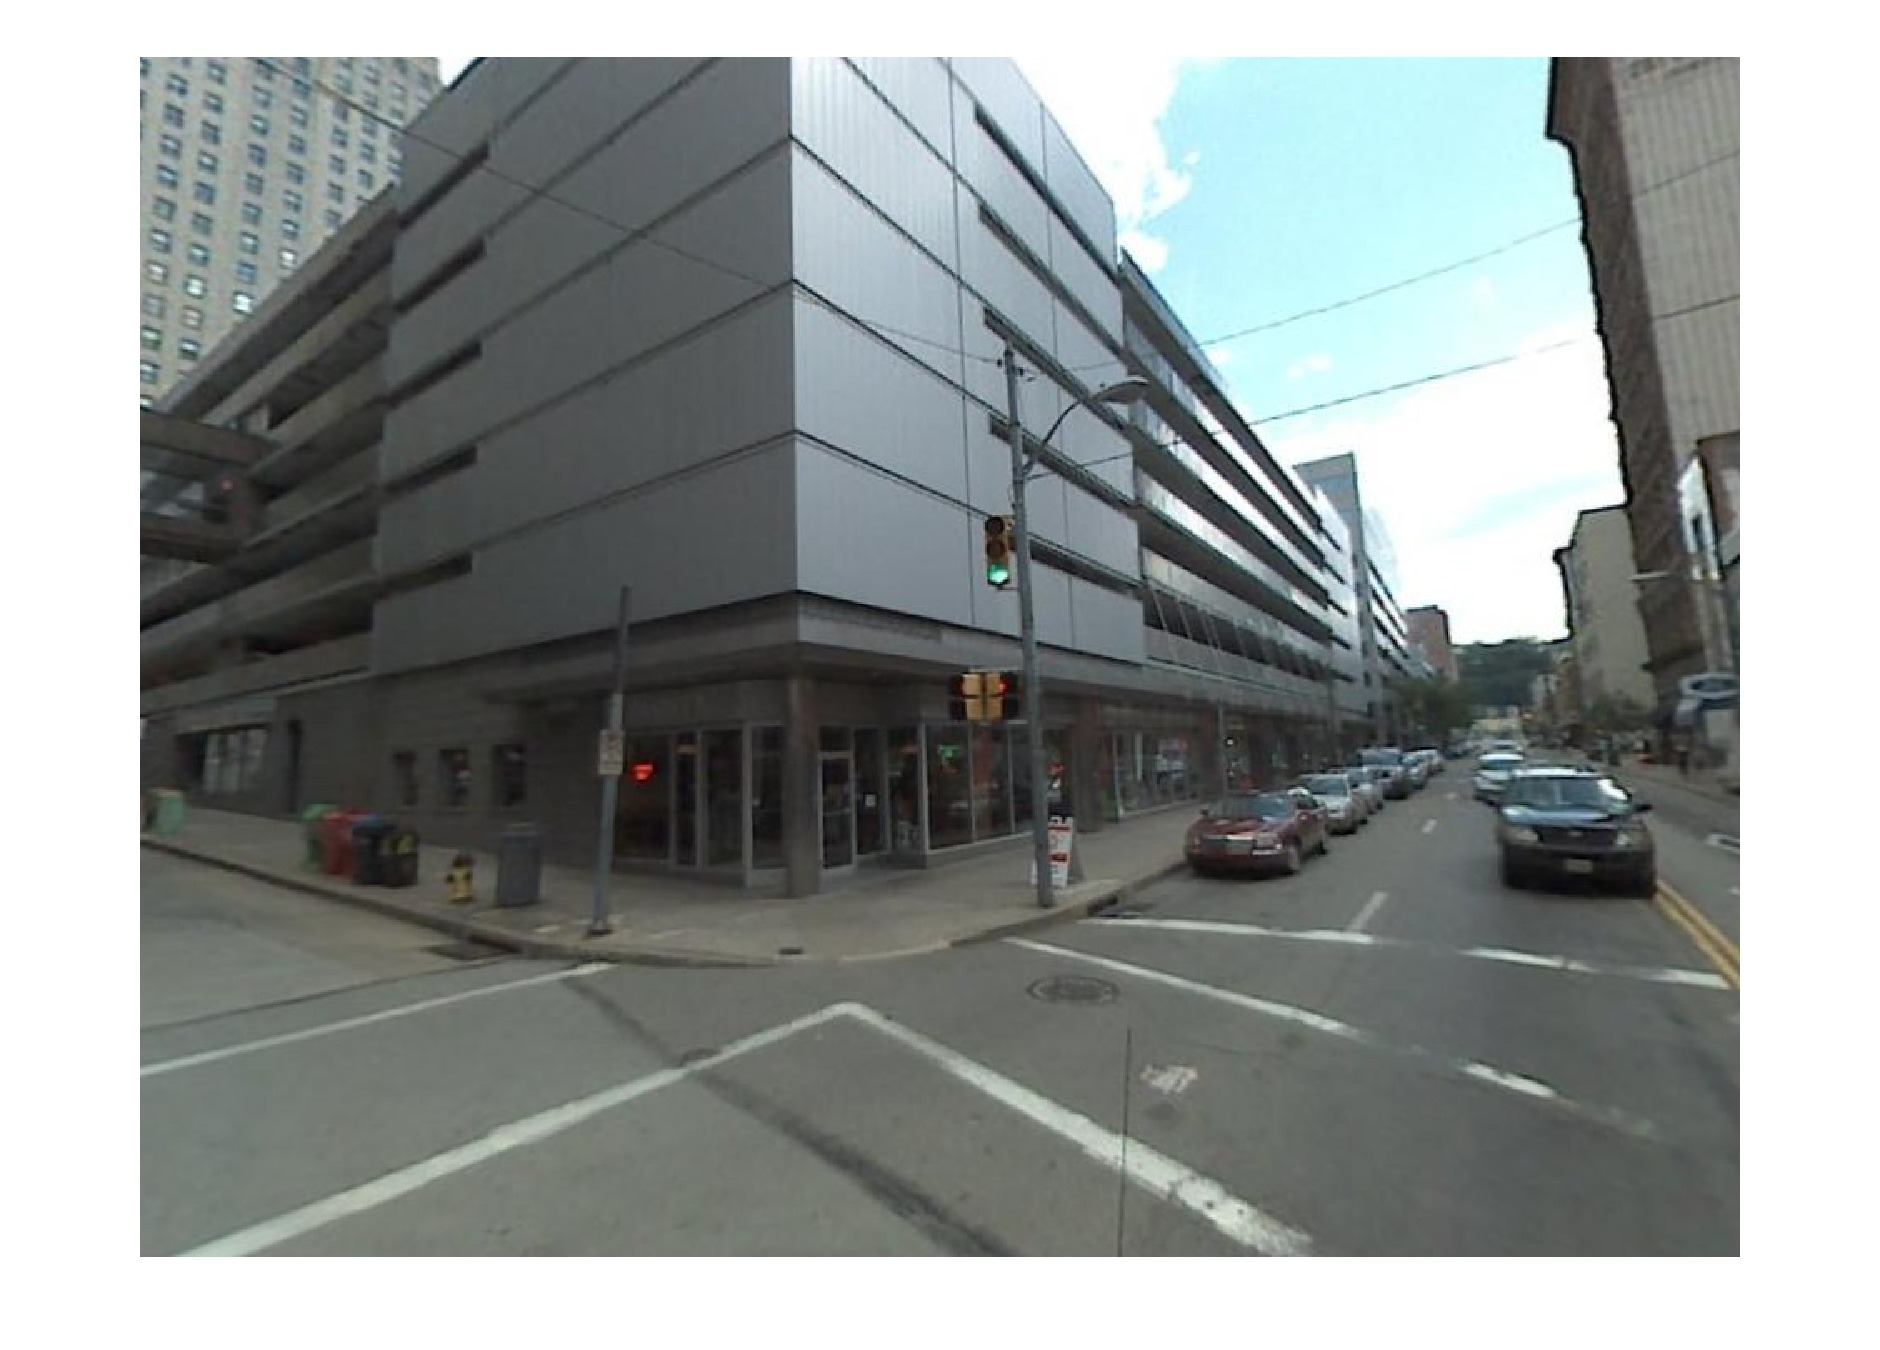
\includegraphics[width=\linewidth]{imgs/wVS3q/2932/a.jpg}
          \end{minipage}  
          \begin{minipage}{\wii}
            \centering
            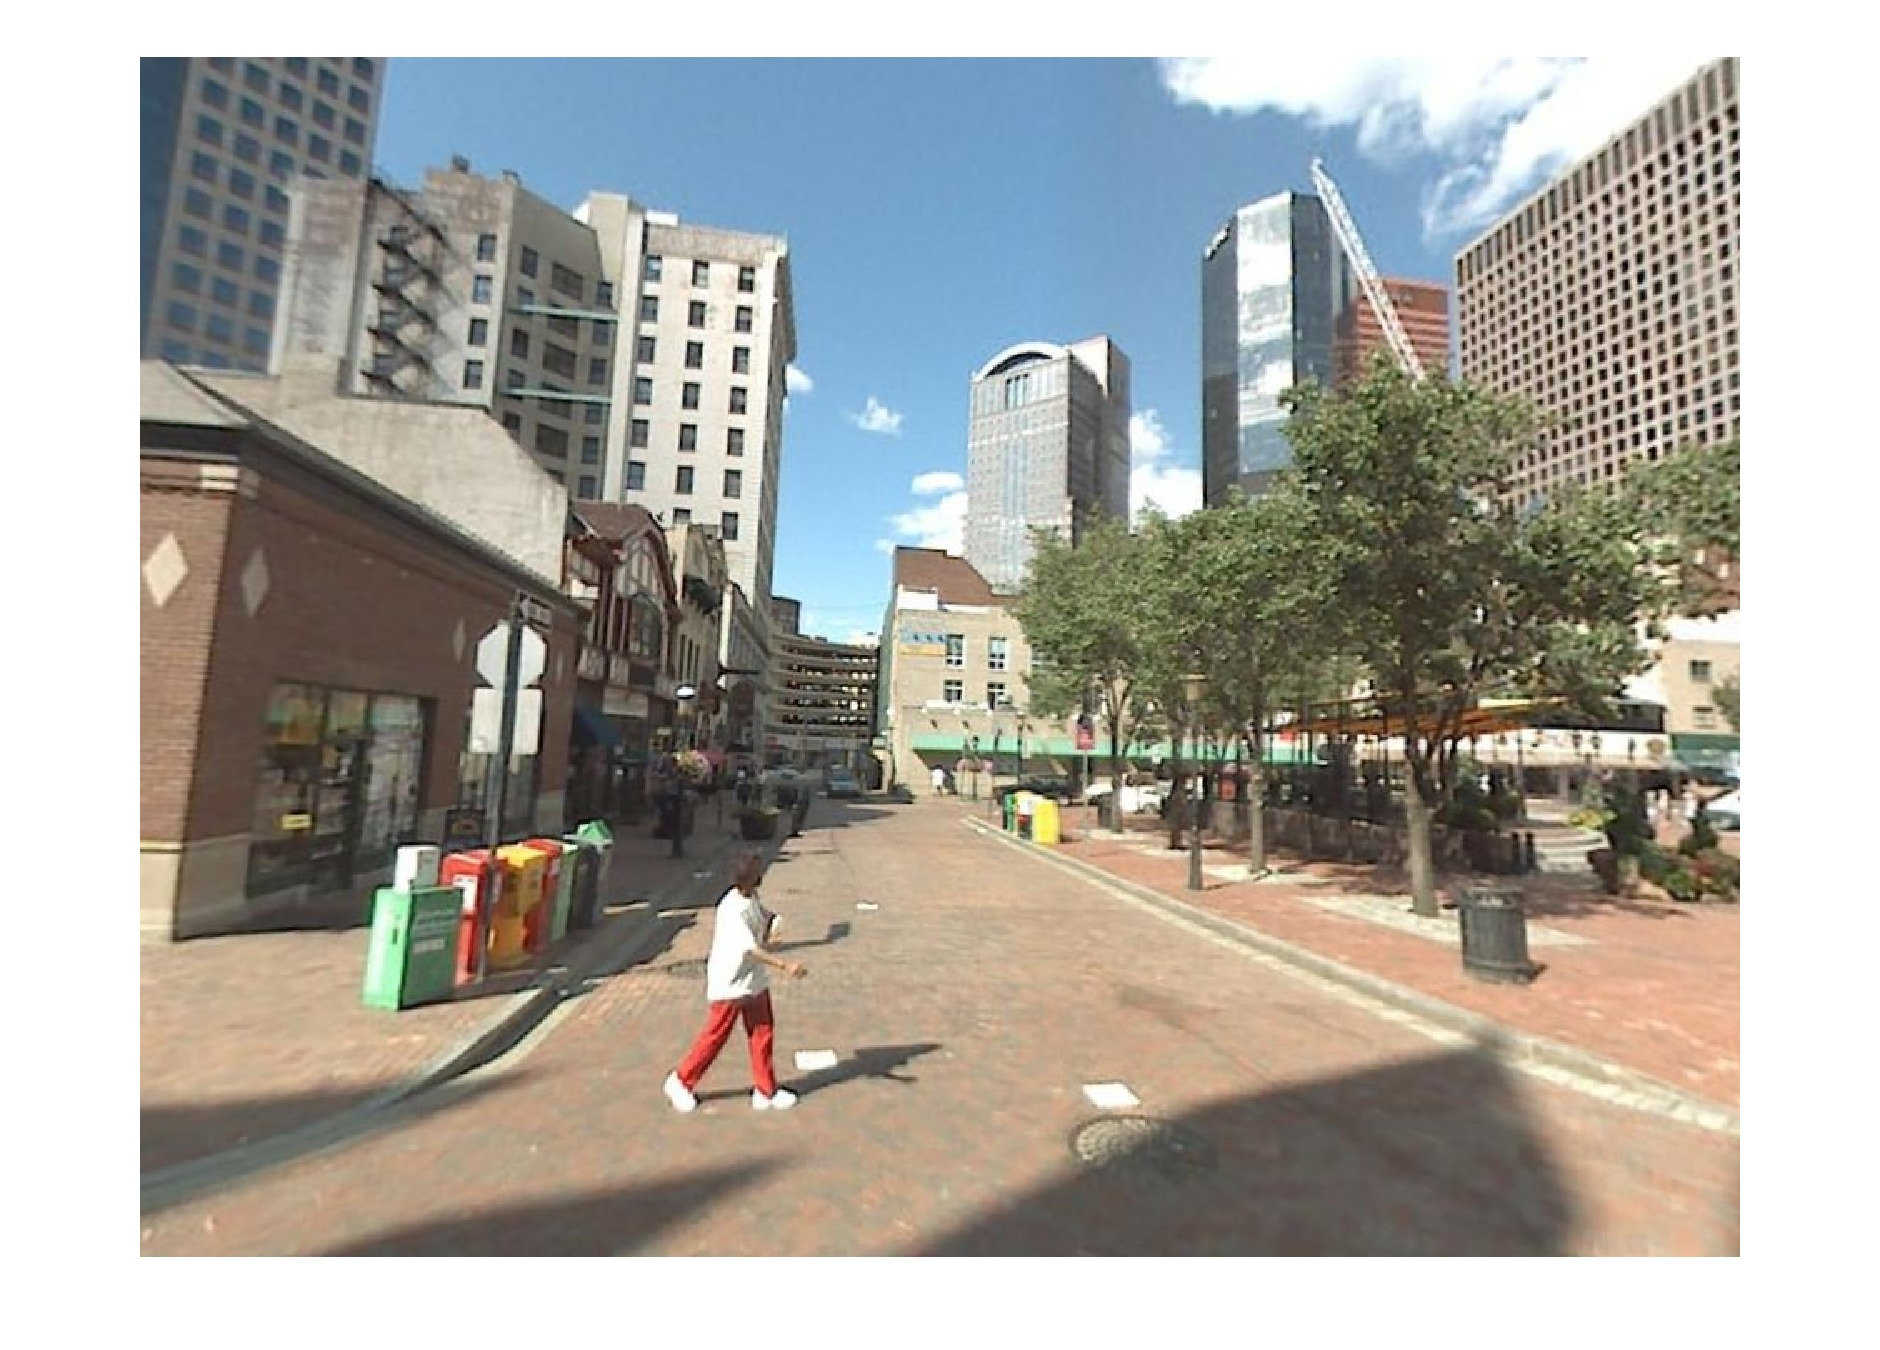
\includegraphics[width=\linewidth]{imgs/wVS3q/2932/b.jpg}
          \end{minipage}  
          \begin{minipage}{\wii}
            \centering
            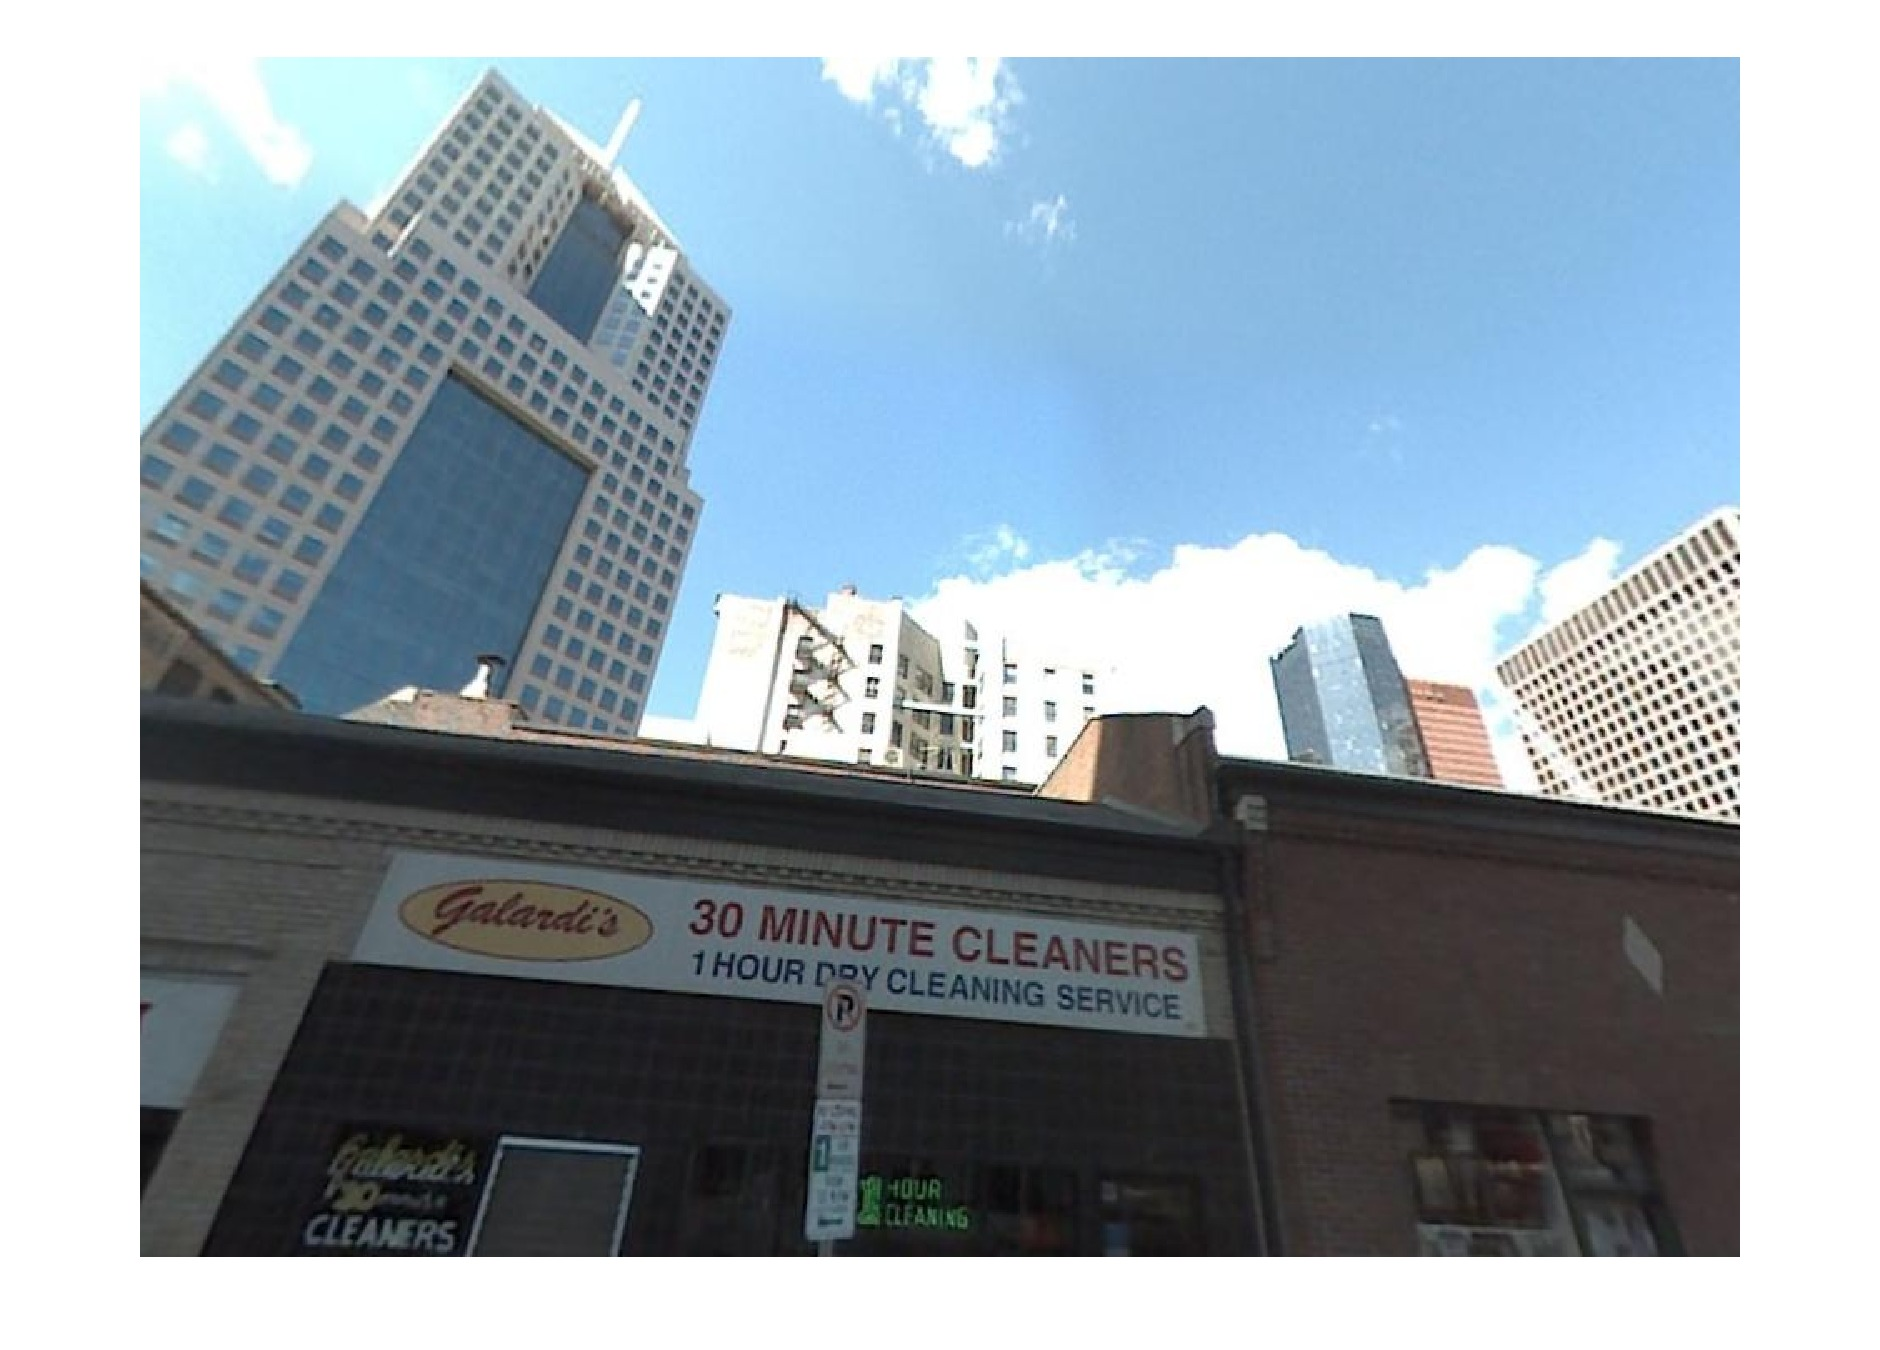
\includegraphics[width=\linewidth]{imgs/wVS3q/2932/c.jpg}
          \end{minipage} 
          \\
          \begin{minipage}{\wii}
            \centering
            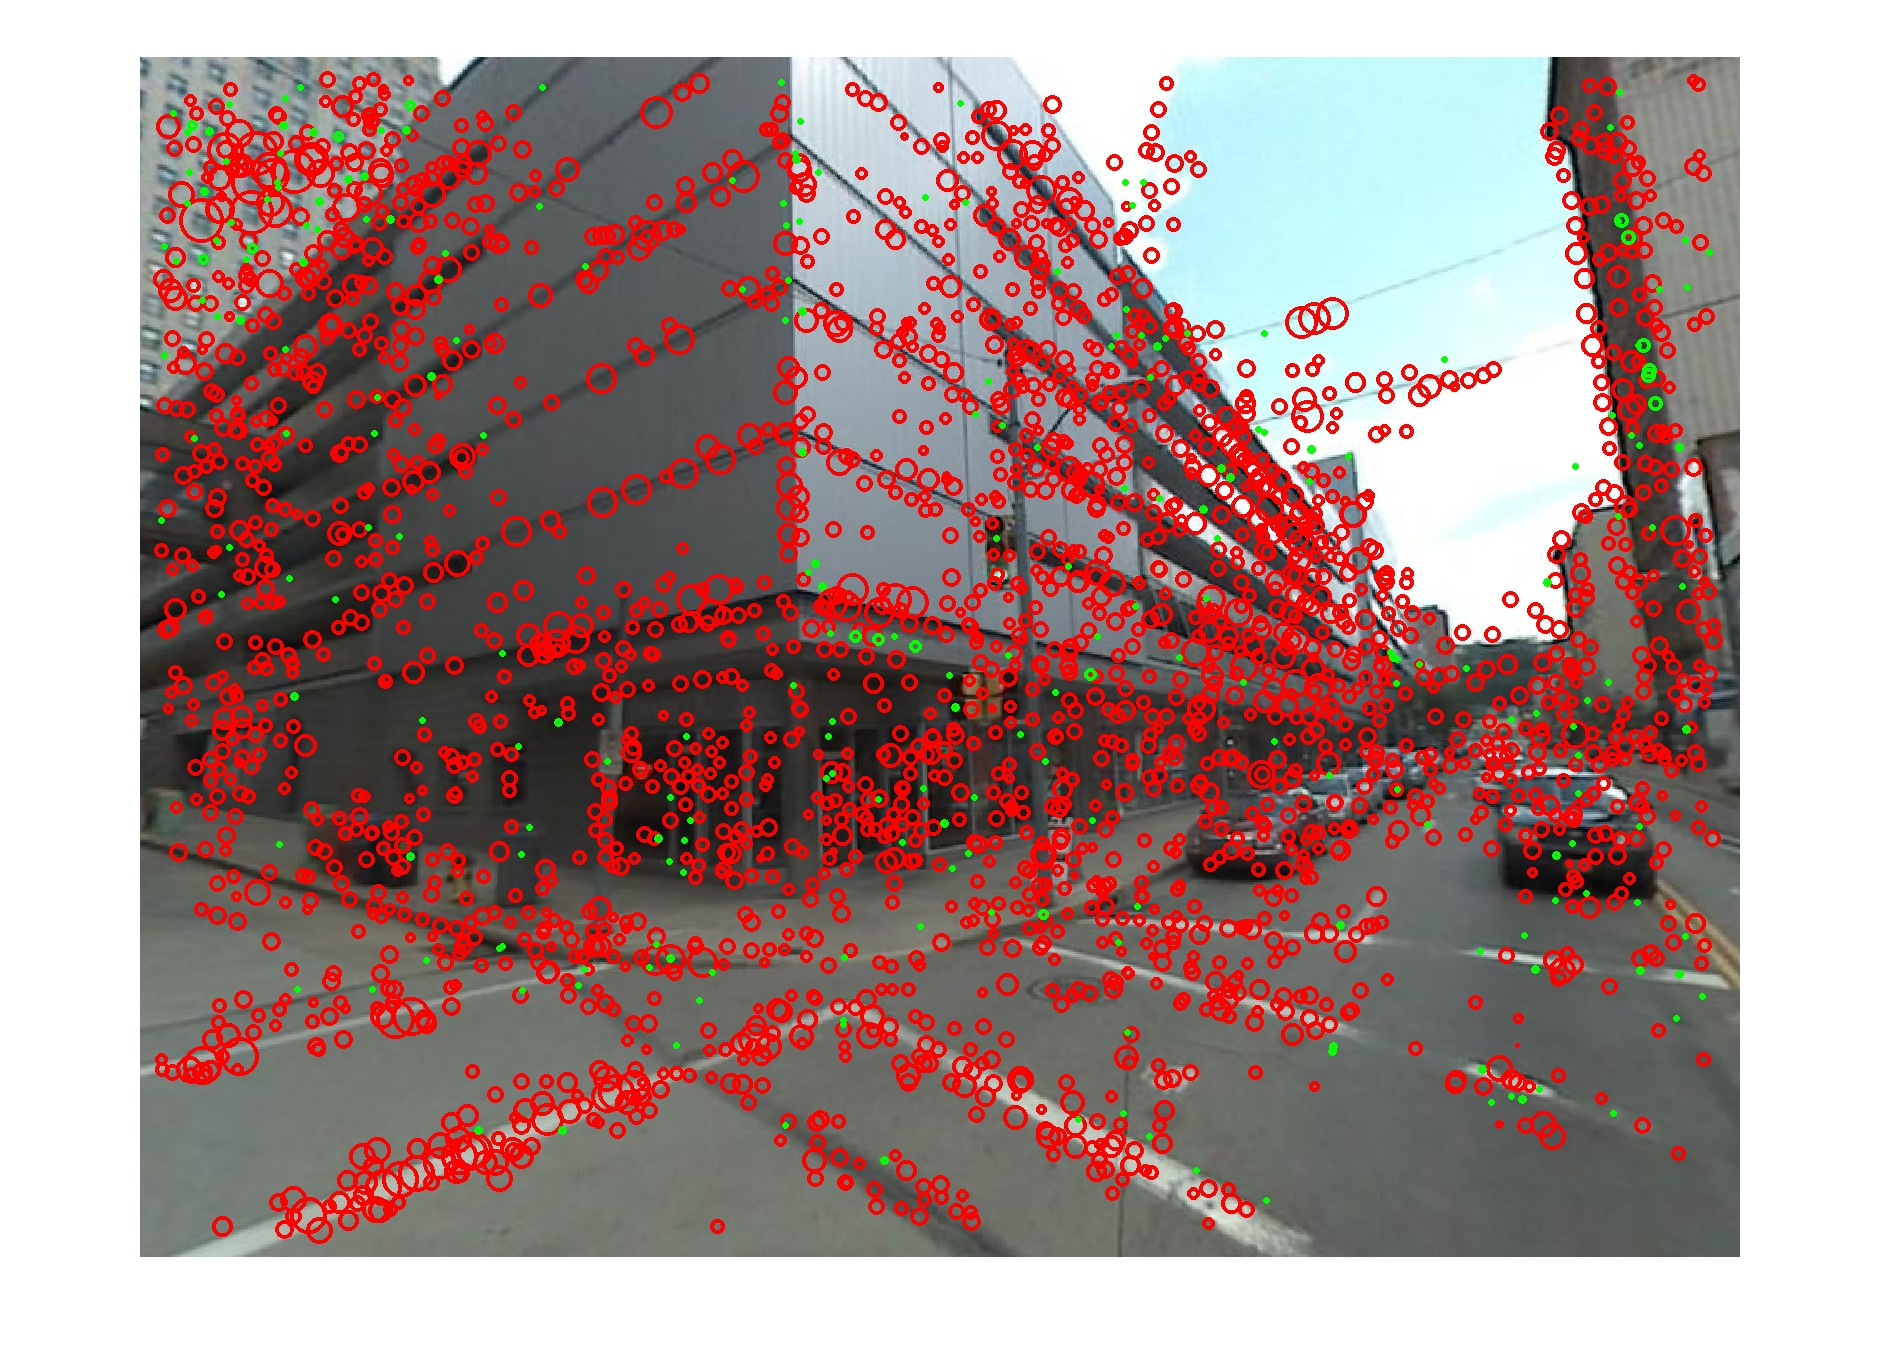
\includegraphics[width=\linewidth]{imgs/wVS3q/2932/aftrs.jpg}
            \newline
            (a)
          \end{minipage}  
          \begin{minipage}{\wii}
            \centering
            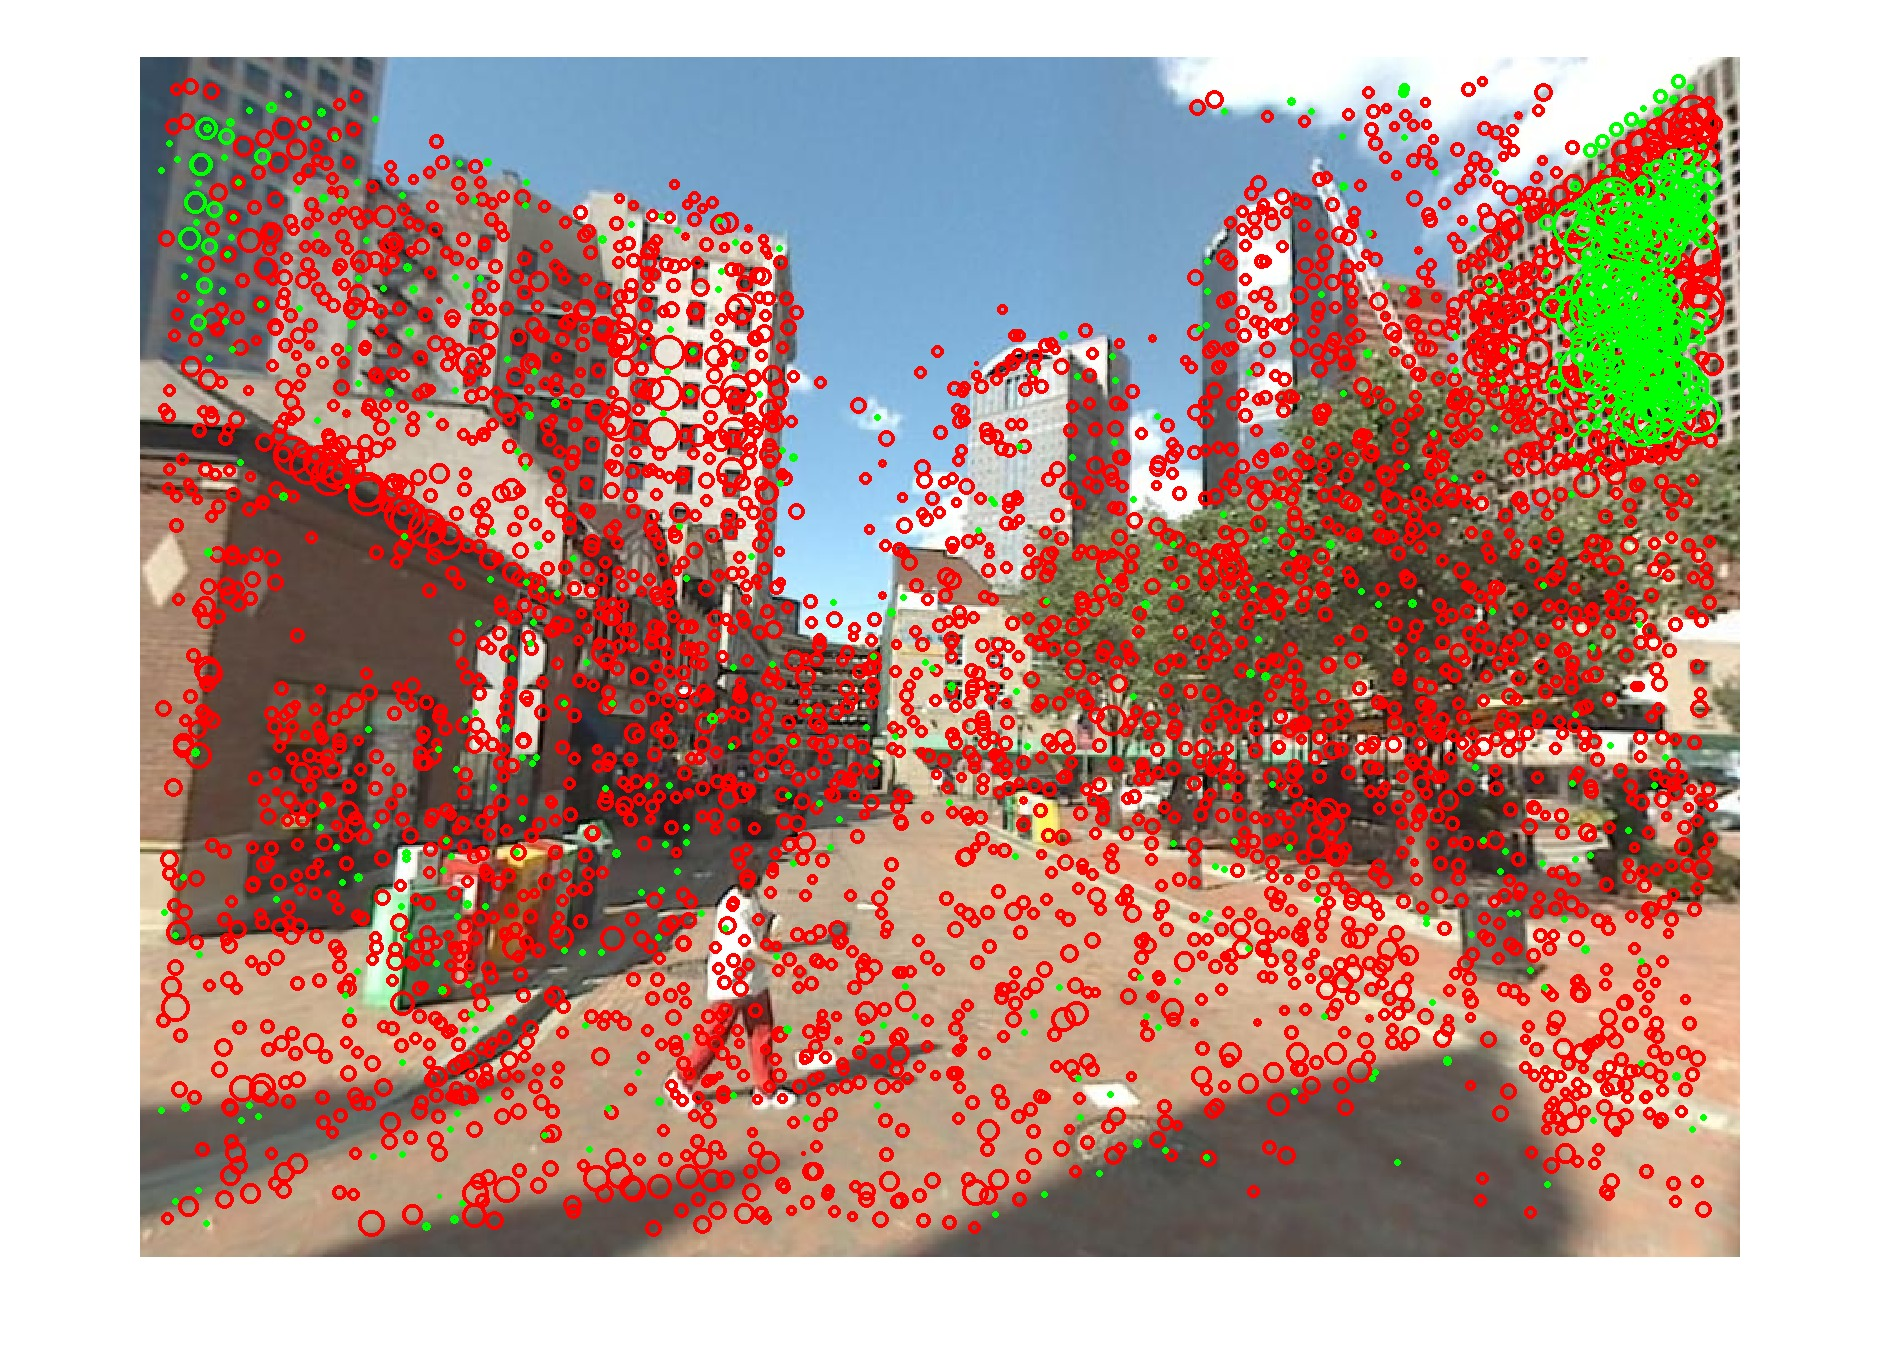
\includegraphics[width=\linewidth]{imgs/wVS3q/2932/bftrs.jpg}
            \newline
            (b)
          \end{minipage}  
          \begin{minipage}{\wii}
            \centering
            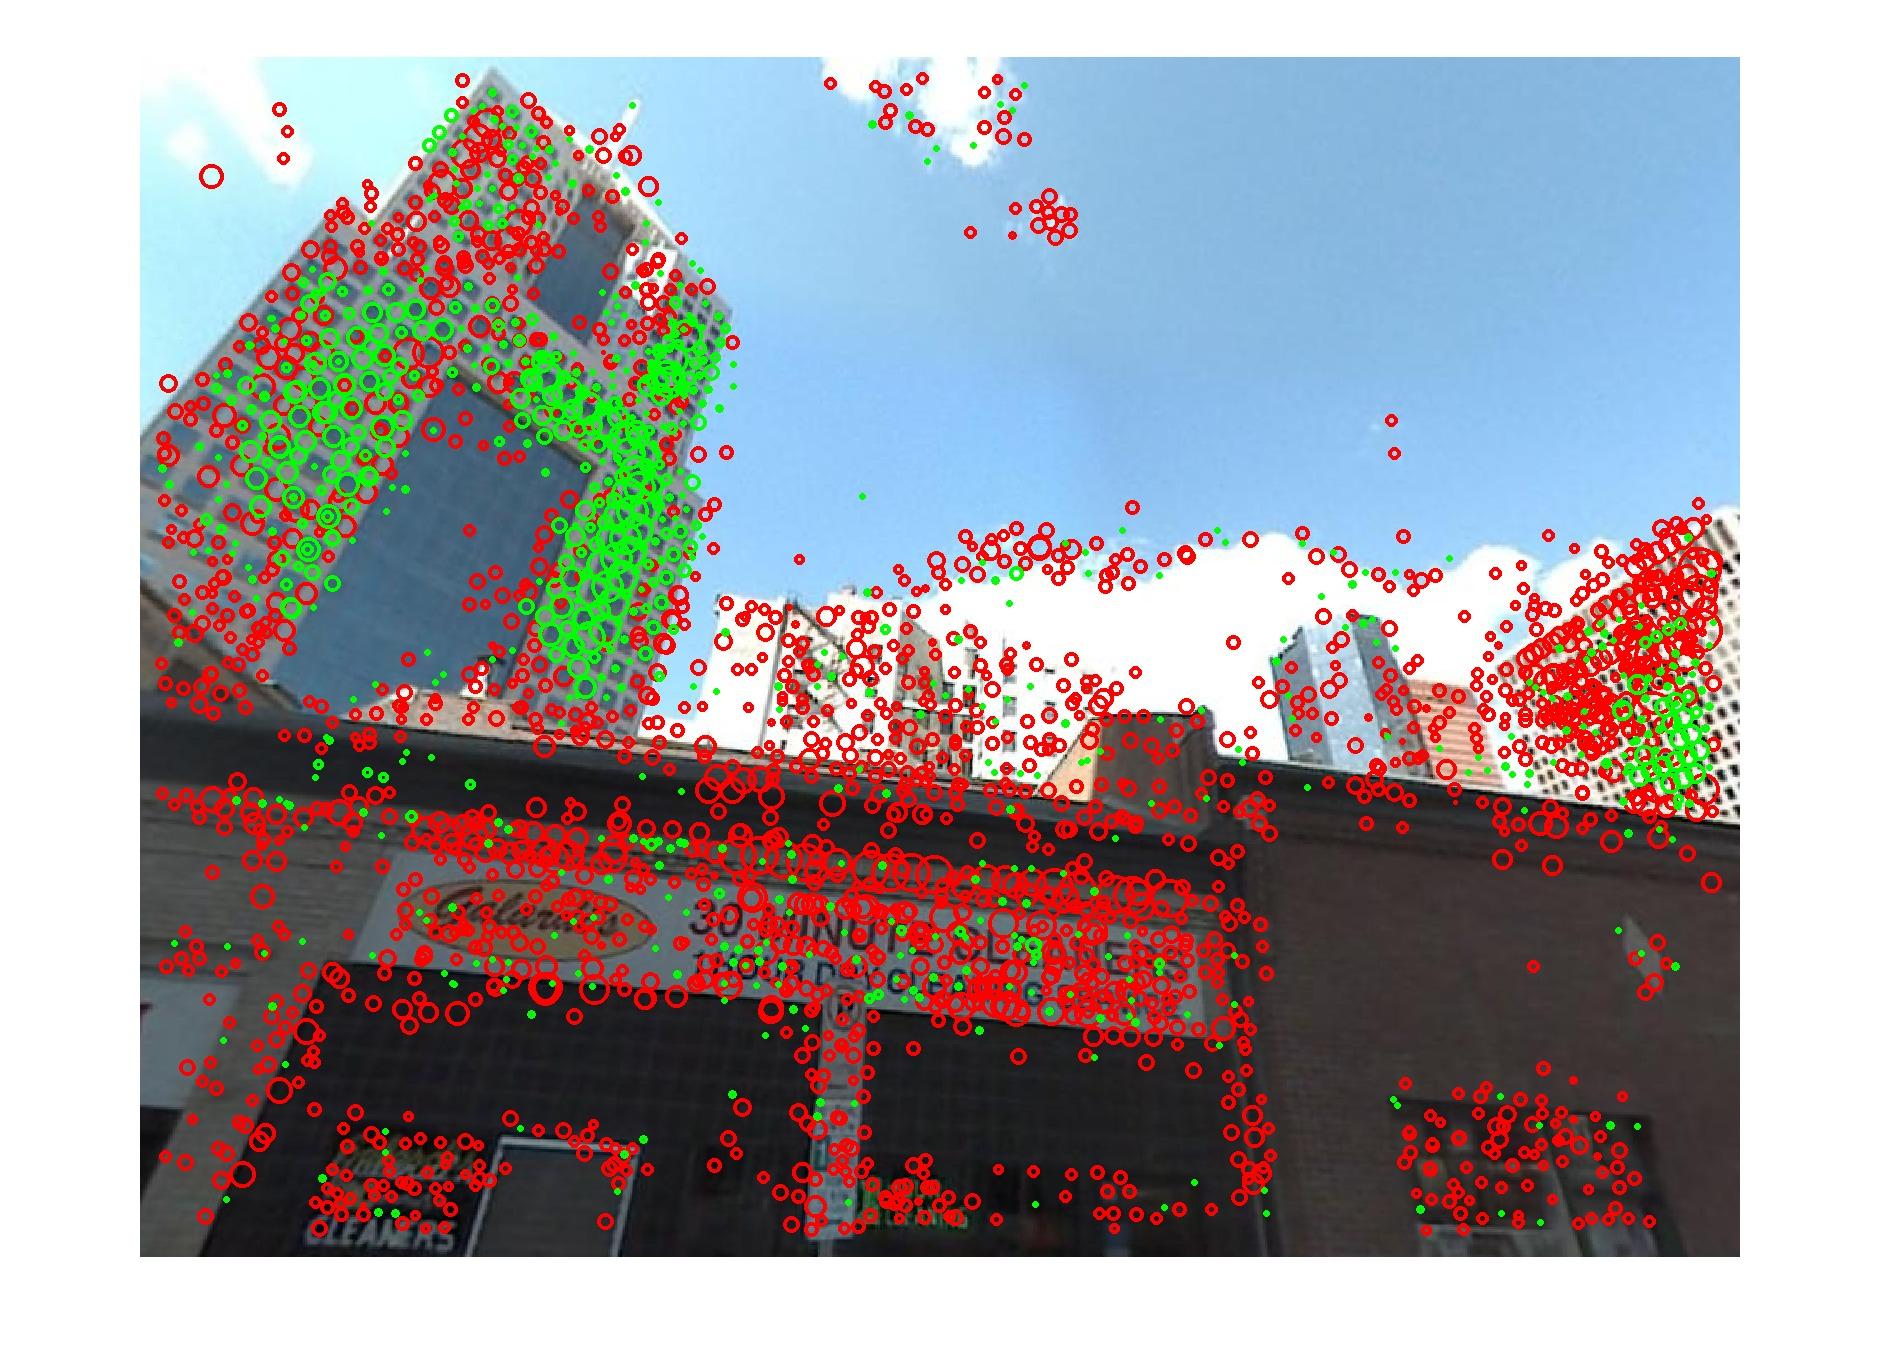
\includegraphics[width=\linewidth]{imgs/wVS3q/2932/cftrs.jpg}
            \newline
            (c)
          \end{minipage} 
    \end{minipage}% right figure
    %
    \vspace*{-2mm}
    \caption{\myCap}
    \label{fig:3qVSw}
        \vspace*{2mm}
    \end{figure*}

% BibTeX users please use one of
%\bibliographystyle{spbasic}      % basic style, author-year citations
%\bibliographystyle{spmpsci}      % mathematics and physical sciences
%\bibliographystyle{spphys}       % APS-like style for physics
%\bibliography{}   % name your BibTeX data base

%\bibliographystyle{spbasic}
%\bibliographystyle{spphys}       % APS-like style for physics
\bibliographystyle{spmpsci}      % mathematics and physical sciences

{\footnotesize
\bibliography{shortstrings,vggroup,cvww_template,mybib}
}
%
%% Non-BibTeX users please use
%\begin{thebibliography}{}
%%
%% and use \bibitem to create references. Consult the Instructions
%% for authors for reference list style.
%%
%\bibitem{RefJ}
%% Format for Journal Reference
%Author, Article title, Journal, Volume, page numbers (year)
%% Format for books
%\bibitem{RefB}
%Author, Book title, page numbers. Publisher, place (year)
%% etc
%\end{thebibliography}

\end{document}
% end of file template.tex

